\documentclass[../main.tex]{subfiles}
%\usepackage[T1]{fontenc}
%\usepackage[utf8]{inputenc}
%\usepackage{geometry}   
%\usepackage{float}
%\usepackage[section]{placeins}
%\usepackage{amsmath}
%\usepackage{amssymb}
%\usepackage{amsfonts}
%\usepackage[colorlinks=true, allcolors=blue]{hyperref}
%\usepackage{mathtools}
%\usepackage[switch, mathlines]{lineno}
%\usepackage[usenames,dvipsnames]{xcolor} 
%\usepackage[normalem]{ulem}
%\usepackage[capitalise,nameinlink]{cleveref}
%\usepackage{enumitem}
%\usepackage{csquotes}
%\usepackage{xspace}
%\usepackage{multirow}
%\usepackage{tabularx}
%\usepackage{color, colortbl}
%\usepackage[colorinlistoftodos]{todonotes}
%\usepackage{graphicx}
%
%% for writing code blocks 
%\usepackage{listings}
%%\usepackage{color}
%\usepackage{caption}
%\usepackage{subcaption}
%\definecolor{orange}{rgb}{1,0.5,0}
%\definecolor{darkorange}{rgb}{0.69,0.33,0.13}
%\definecolor{fidcol}{rgb}{0.7,0,0}
%\definecolor{mkcol}{rgb}{0.5,0,0.5}
%\definecolor{mmcol}{rgb}{0.7,0.17,0.31}
%\definecolor{dscol}{rgb}{0.6,0.1,0.2}
%\definecolor{mccol}{rgb}{0.2,0.4,0.6}
%\definecolor{darkgreen}{rgb}{0.05,0.5,0.06}
%\definecolor{carnelian}{rgb}{0.7, 0.11, 0.11}
%\definecolor{dkgreen}{rgb}{0,0.6,0}
%\definecolor{mauve}{rgb}{0.58,0,0.82}
%\definecolor{gray}{gray}{0.9}
%\definecolor{cyan}{rgb}{0.88,1,1}
%
%\newcommand*{\Euclid}{\textit{Euclid}\xspace}
%\newcommand*{\Planck}{\textit{Planck}\xspace}
%\newcommand*{\rd}{\mathrm{d}}
%\newcommand*{\rD}{\mathrm{D}}
%\newcommand*{\marktodo}{{\color{mmcol} ::TODO::}\xspace}
%\newcommand*{\halofit}{\texttt{HALOFIT}\xspace}
%\newcommand*{\hmcode}{\texttt{HMCODE}\xspace}
%\newcommand*{\montepython}{\texttt{MP}\xspace}
%\newcommand*{\cosmicfish}{\texttt{CF}\xspace}
%\newcommand*{\class}{{\tt CLASS}\xspace}
%\newcommand*{\camb}{{\tt CAMB}\xspace}
%\newcommand*{\montefisher}{\texttt{MP:Fisher}\xspace}
%
%\newcommand*{\neff}{N_\mathrm{eff}}
%
\begin{document}
\chapter{Validation of the Forecasting Pipeline}\label{cha:validate}
Our main goal is a validated and robust sensitivity forecast for the neutrino parameters of \Euclid. For this, we have adopted a validation pipeline from \cite{casas2023euclid}. It starts with the code \cosmicfish that was validated in the \Euclid project \cite{Euclid:2019clj}. In this work, we have modified the recopies of the nonlinear modelling and modelling of the neutrino-induced scale-dependent growth to better describe the effect of massive neutrinos. Thus, we decided to do a re-validation of the \montepython pipeline. We will also check how well the Fisher formalism works for the neutrino mass that is close to a theoretical prior at zero mass.\\
In this section, we choose a different model that we will use in the final forecasting results to have posteriors that are Gaussian enough to be able to be approximated using the FI methods. The parameters are given in table \ref{tab:fiducial_validation}.
\begin{table}[t]
    \renewcommand{\arraystretch}{1.2}
        \caption{Fiducial values of the parameters varied in the validation section. The $\Lambda$CDM parameters were always varied during the Validation runs while the extended Models were only varied two at a time. The meaning parameters are described in the text.}
        \centering
        %\resizebox{\textwidth}{!}{
        \begin{tabular}{ccccc|cccc}
        \hline
        \rowcolor{cyan} \multicolumn{9} {c}{{\bf{Fiducial}}}\\ 
         \rowcolor{gray}    \multicolumn{5} {c}{$\Lambda$CDM} & \multicolumn{4} {|c}{Extensions} \\
     \multicolumn{1}{c}{$\Omega_{\rm m,0}$} & \multicolumn{1}{c}{$100\times\Omega_{\rm b,0}$} & \multicolumn{1}{c}{$h$} & \multicolumn{1}{c}{$n_{\rm s}$} & \multicolumn{1}{c}{$\sigma_{8}$} & \multicolumn{1}{|c}{$m_\nu$(meV)} & \multicolumn{1}{c}{$\neff$} & \multicolumn{1}{c}{$w_0$} & \multicolumn{1}{c}{$w_a$} \\
      \hline
            0.314571 & 4.92 & $0.6737$ & $0.9661$ & $0.81$ & $60$ & $3.044$ & $0$ & $-1$ \\
        \end{tabular}
        %}
        \label{tab:fiducial_validation}
    \end{table}

The extensions to the $\Lambda$CDM models in this section are varied in pairs of two. We first look at a model where we vary $w_0+w_a$. These parameters are an approximation to a dark energy equation of state that is slowly varying. It is parametrized as having $w(a) = w_0 + w_a(1-a)$. We note that when fixing the parameters to their fiducial values, we recover $\Lambda$CDM. This $w_0w_a$CDM model was the original model that was validated in the work of \. We kept it in our validation pipeline to be sure that we did not break the previous validation with our changes to the pipeline.\\
The second model that we look at is a model where we vary the constant pressure-to-density ratio of dark energy $w_0$ (fixing $w_a$) and the approximated neutrino mass $m_\nu$. We will use the symbol $m_\nu$ in this section rather than $\sum m_\nu$ to denote this quantity as in our parametrization we approximate that all the neutrino mass is concentrated into one massive neutrino with a temperature of \begin{equation}
    \frac{T_\nu}{T_\gamma} = \left(\frac{4}{11}\right)^{1/3}\,\left(\frac{3.044}{3}\right)^{1/4} = 0.716369.
\end{equation}  
This is different from the parametrization of \cite{casas2023euclid}. In their parametrisation, the neutrino temperature had a factor of $\neff$ in their second factor instead of its fiducial value. In that sense their parameter $\neff$ is different from ours as it was partly accounting for additional $\neff$ to a higher neutrino temperature. For us, $\neff$ is accounting for additional massless degrees of freedom and thus a higher value of $\neff$ does not also mean a higher energy density of massive neutrinos.\\
We also note that this approximated mass of massive neutrinos is also not exactly the mass of a massive neutrino because it is the mass of a neutrino in an instantaneous decoupling approximation. It corresponds to a neutrino density fraction, $\Omega_\nu$, of 
\begin{equation}
    \label{eq:omega_nu}
    \Omega_\nu\,h^2= \frac{m_\nu}{94.07\,\mathrm{eV}}\,\left(\frac{3.044}{3}\right)^{3/4} = \frac{m_\nu}{0.06\,\mathrm{eV}}\,6.44826\cdot10^{-4}
\end{equation}
In reality the factor of $94.07\,\mathrm{eV}$ in the denominator of the first factor would be given through an integral over the neutrino phase space distribution. To better match the parametrization between our two EBS \class and \camb, we stick to the instantaneous decoupling approximation done in \camb. We do this by internally converting the input neutrino mass in \class to $\Omega_\nu$ with the approximate equation. The change to the neutrino temperature propagates to this equation, as the second factor is proportional to the neutrino temperature.\\
In the third model, we fix the dark energy equation of state to its $\Lambda$CDM value and vary the approximated neutrino mass and the effective relativistic degrees of freedom. As we stated before our changes to the neutrino parametrization make the value of $\neff$ correspond to the actual numbers of massless species $N_\mathrm{ur}$. We can translate these quantities in this case to another by \begin{equation}
    N_\mathrm{ur} = \neff - \frac{3.044}{3},
\end{equation}
where the second term stands for the one massive neutrino. In the actual forecasting results, we will change our neutrino parametrization to have three massive neutrinos with degenerate masses. In this case, we will subtract three times that from the $\neff$, such that the parameter will correspond to any additional species of massless relics particles. We will denote this quantity as $\Delta \neff$ with a theoretical prior bound at zero.\\
In all the validation models we have fixed the modelling parameters of nonlinear effects in the spectroscopic probe, namely $\sigma_p$ and $\sigma_v$, to their fiducial values. This is done because especially $\sigma_p$ is very degenerate with the cosmological parameter, breaking the Gaussian approximation needed for the FI method.\\
We will validate our pipeline separately for both main probes of the \Euclid mission, for both the optimistic and pessimistic settings and all three models totalling twelve total tests. The tests itself are done in three steps \begin{itemize}
    \item[-] We will first validate our EBS implementation by validating the FI results of \cosmicfish for the two codes \camb and \class.
    \item[-] We will then validate our likelihood implementation by validating those two results with the FI obtained by \montepython in Fisher mode.
    \item[-] We will test for the validity of the Gaussian approximation by comparing the obtained FI matrices with the posteriors obtained by an MCMC run in \montepython with the Metropolis-Hastings algorithm.    
\end{itemize}
In the last step, by construction, there is no possibility of a theoretical error showing up as the same likelihood is used to generate the MCMC to calculate the FI matrix. We decide that our implementation is validated when the marginalized and unmarginalized one-dimensional errors are within 10\% of the median. This validation criterion is taken from the previous \Euclid validation standard from \cite{casas2023euclid}.\\
This chapter will be structured in the following way. Firstly, we discuss the precision settings for the two Einstein-Boltzmann solvers(EBS) \camb and \class that we need to set to get their fiducial power spectra to match to sub-percent level. We will then show the agreement of the three different FI matrices and discuss their stability under change of stepsizes and derivation methods. In the next step, we will then compare the FI matrices with the MCMC results and try to explain the derivations. In the last section, we discuss the effect of nonlinear modelling and analyze possible biasing.
\section{The Einstein-Bolzmann Solvers}
To match the results from the two EBS we needed to first understand the differences between codes. The first difference was already alluded to in the introduction to this section. \camb uses the phase space integral for the neutrinos in the limit of instantaneous decoupling while \class uses a slightly different value taking into account relic scattering and neutrino oscillations. To circumvent this problem we added a new parameter {\tt m\_nu\_camb} that is converted to the neutrino density fraction $\Omega_\nu$ via equation \ref{eq:omega_nu}, before each call of \class .\\
The total matter density parameter $\Omega_m$ is also defined slightly differently in \camb and \class. While \camb defines the total matter density as CDM+baryons+massive neutrinos, \class does not include the massive neutrinos. To match the codes we defined a new parameter {\tt Omega\_m\_camb} that is converted to the density parameter of cold dark matter, $\Omega_{c}$, before the run by subtracting the other two ingredients.\\
Another detail in our implementation was that \camb is not able to use $\sigma_8$ as an input parameter. This is because it is computed from the linear matter power spectrum. In \class, we have a shooting functionality where we use a reference value of $A_s$ to calculate $\sigma_8$. As $\sigma_8$ is directly proportional to $A_s$, by rescaling $A_s$ we can match the desired value of $\sigma_8$. Since this functionality does not exist in \camb, we mimic the shooting by doing a first reference run of CAMB to obtain the matter power spectrum and then rescale to match $\sigma_8$ inside \cosmicfish. With these three modifications, we were able to match the input parameters between \class and \camb.\\
The next step in the validation of the EBS is a careful choice of the accuracy settings. This is done such that \begin{enumerate}
    \item[A:] The power spectra are numerically stable enough such that their derivatives are not dominated by noise,
    \item[B:] Small differences in the approximation schemes of the EBS do not propagate to the final forecasting results.   
\end{enumerate} The choice of the accuracy settings inside \camb is simple. There are generic parameters that boost the accuracy of the \camb code in multiple different places.
We decided to use the following accuracy settings in \camb.  
\begin{lstlisting}[language=Python,caption=\camb:HP precision settings]
    do_late_rad_truncation = T
    high_accuracy_default = T
    transfer_interp_matterpower = T
    accurate_reionization = F
    accuracy_boost = 3
    l_accuracy_boost = 3
    accurate_massive_neutrino_transfers = T
\end{lstlisting} 
In the rest of the discussion, these settings will be called \camb:HP. The intrinsic accuracy settings in the code, like integration cutoffs, truncation of the Boltzmann hierarchy, and stepsizes, are all multiplied by the corresponding accuracy boost. The parameter {\tt do\_late\_rad\_truncation} truncates the Boltzmann hierarchy for radiation at high $\ell$ after matter domination. The option for {\tt accurate\_massive\_neutrino\_transfers} allows us to obtain the neutrino transfer functions that are needed in the modelling of our photometric probe.\\
The high-precision settings that we chose in \class are summarized in the following.

\begin{lstlisting}[language=Python,caption=\class:HP precision settings, label=lst:classHP]
    k_per_decade_for_bao = 50
    k_per_decade_for_pk = 50
    l_max_g = 20
    l_max_pol_g = 15
    radiation_streaming_approximation = 2
    radiation_streaming_trigger_tau_over_tau_k = 240.
    radiation_streaming_trigger_tau_c_over_tau = 100.
    tol_ncdm_synchronous = 1.e-5
    background_Nloga = 6000
    thermo_Nz_log = 20000
    thermo_Nz_lin = 40000
    tol_perturbations_integration = 1.e-6
    halofit_tol_sigma = 1.e-8
    l_max_ncdm = 25
    ncdm_fluid_trigger_tau_over_tau_k = 100.
\end{lstlisting} 
 The approximation schemes of \class are described in \cite{Blas:2011rf}. In \class, we truncate the Boltzmann hierarchy for our ultra-relativistic species, i.e. photons and neutrinos, like in \camb. This cutoff is governed by the precision parameters {\tt l\_max\_xxx}, where {\tt xxx} stands for the species.\\
 Once deep inside the Hubble horizon we further simplify the equations of radiation and light relics by doing a fluid approximation. A fluid approximation means that we approximate the species as an imperfect fluid with anisotropic stress. This essentially truncates the Boltzmann hierarchy at 2 by exponentially suppressing higher moments. For our massive neutrino, the time of this approximation is governed by the parameter {\tt ncdm\_fluid\_trigger\_tau\_over\_tau\_k}.
 The fluid approximation is not present in \camb.\\
  To match the output of the two codes we have to deactivate the fluid approximation. This is done by passing the parameter {\tt ncdm\_fluid\_approximation=3}. We further found that the effect of the fluid approximation is negligible in the highly nonlinear regime. This is why we decided to use a different set of precision parameters in the validation of the different probes. For the photometric probe, we stick to the \class:HP settings while for the spectroscopic probe, we have adjusted our setting to the ultra-high precision settings \class:UHP.
 \begin{lstlisting}[language=Python,caption=\class:UHP precision settings, label=lst:classUHP]
    k_per_decade_for_bao = 50
    k_per_decade_for_pk = 50
    l_max_g = 20
    l_max_pol_g = 15
    radiation_streaming_approximation = 2
    radiation_streaming_trigger_tau_over_tau_k = 240.
    radiation_streaming_trigger_tau_c_over_tau = 100.
    tol_ncdm_synchronous = 1.e-5
    background_Nloga = 6000
    thermo_Nz_log = 20000
    thermo_Nz_lin = 40000
    tol_perturbations_integration = 1.e-6
    halofit_tol_sigma = 1.e-8
    l_max_ncdm = 40
    ncdm_fluid_appoxmation = 3.
    evolver = 0
 \end{lstlisting}
 The two precision settings in listings \ref{lst:classHP} and \ref{lst:classUHP} differ by three parameters. Firstly, the truncation of the Boltzmann hierarchy for massive neutrinos happens at a higher $\ell=40$. This is done to better match the cutoff of \camb. With our precision settings, the truncation happens at a high $\ell$ of 75. The second change is the deactivation of the neutrino fluid approximation and the last one is the change of the evolver. The change from our high precision setting to the ultra-high precision settings makes \class very slow. The standard evolver for a typical call of the code takes the order of tens of minutes. By switching the evolver from the stiff ndf15 evolver to a standard Runge-Kutta integrator we could cut down the computation time to approximately 20\%.\\
 Finally, when running the MCMCs we can set the precision parameters back to the \class defaults. The changes that the precision parameters make only affect the final power spectrum at the per mille level. As this only propagates to small changes in the final likelihood, the MCMC is unaffected by our precision parameters. The default precision parameters are denoted by us with \class:DP.\\
 We present our Comparison between the different power spectra obtained by our EBS in figure \ref{fig:precisson_settings}.
 \begin{figure}
    \centering
    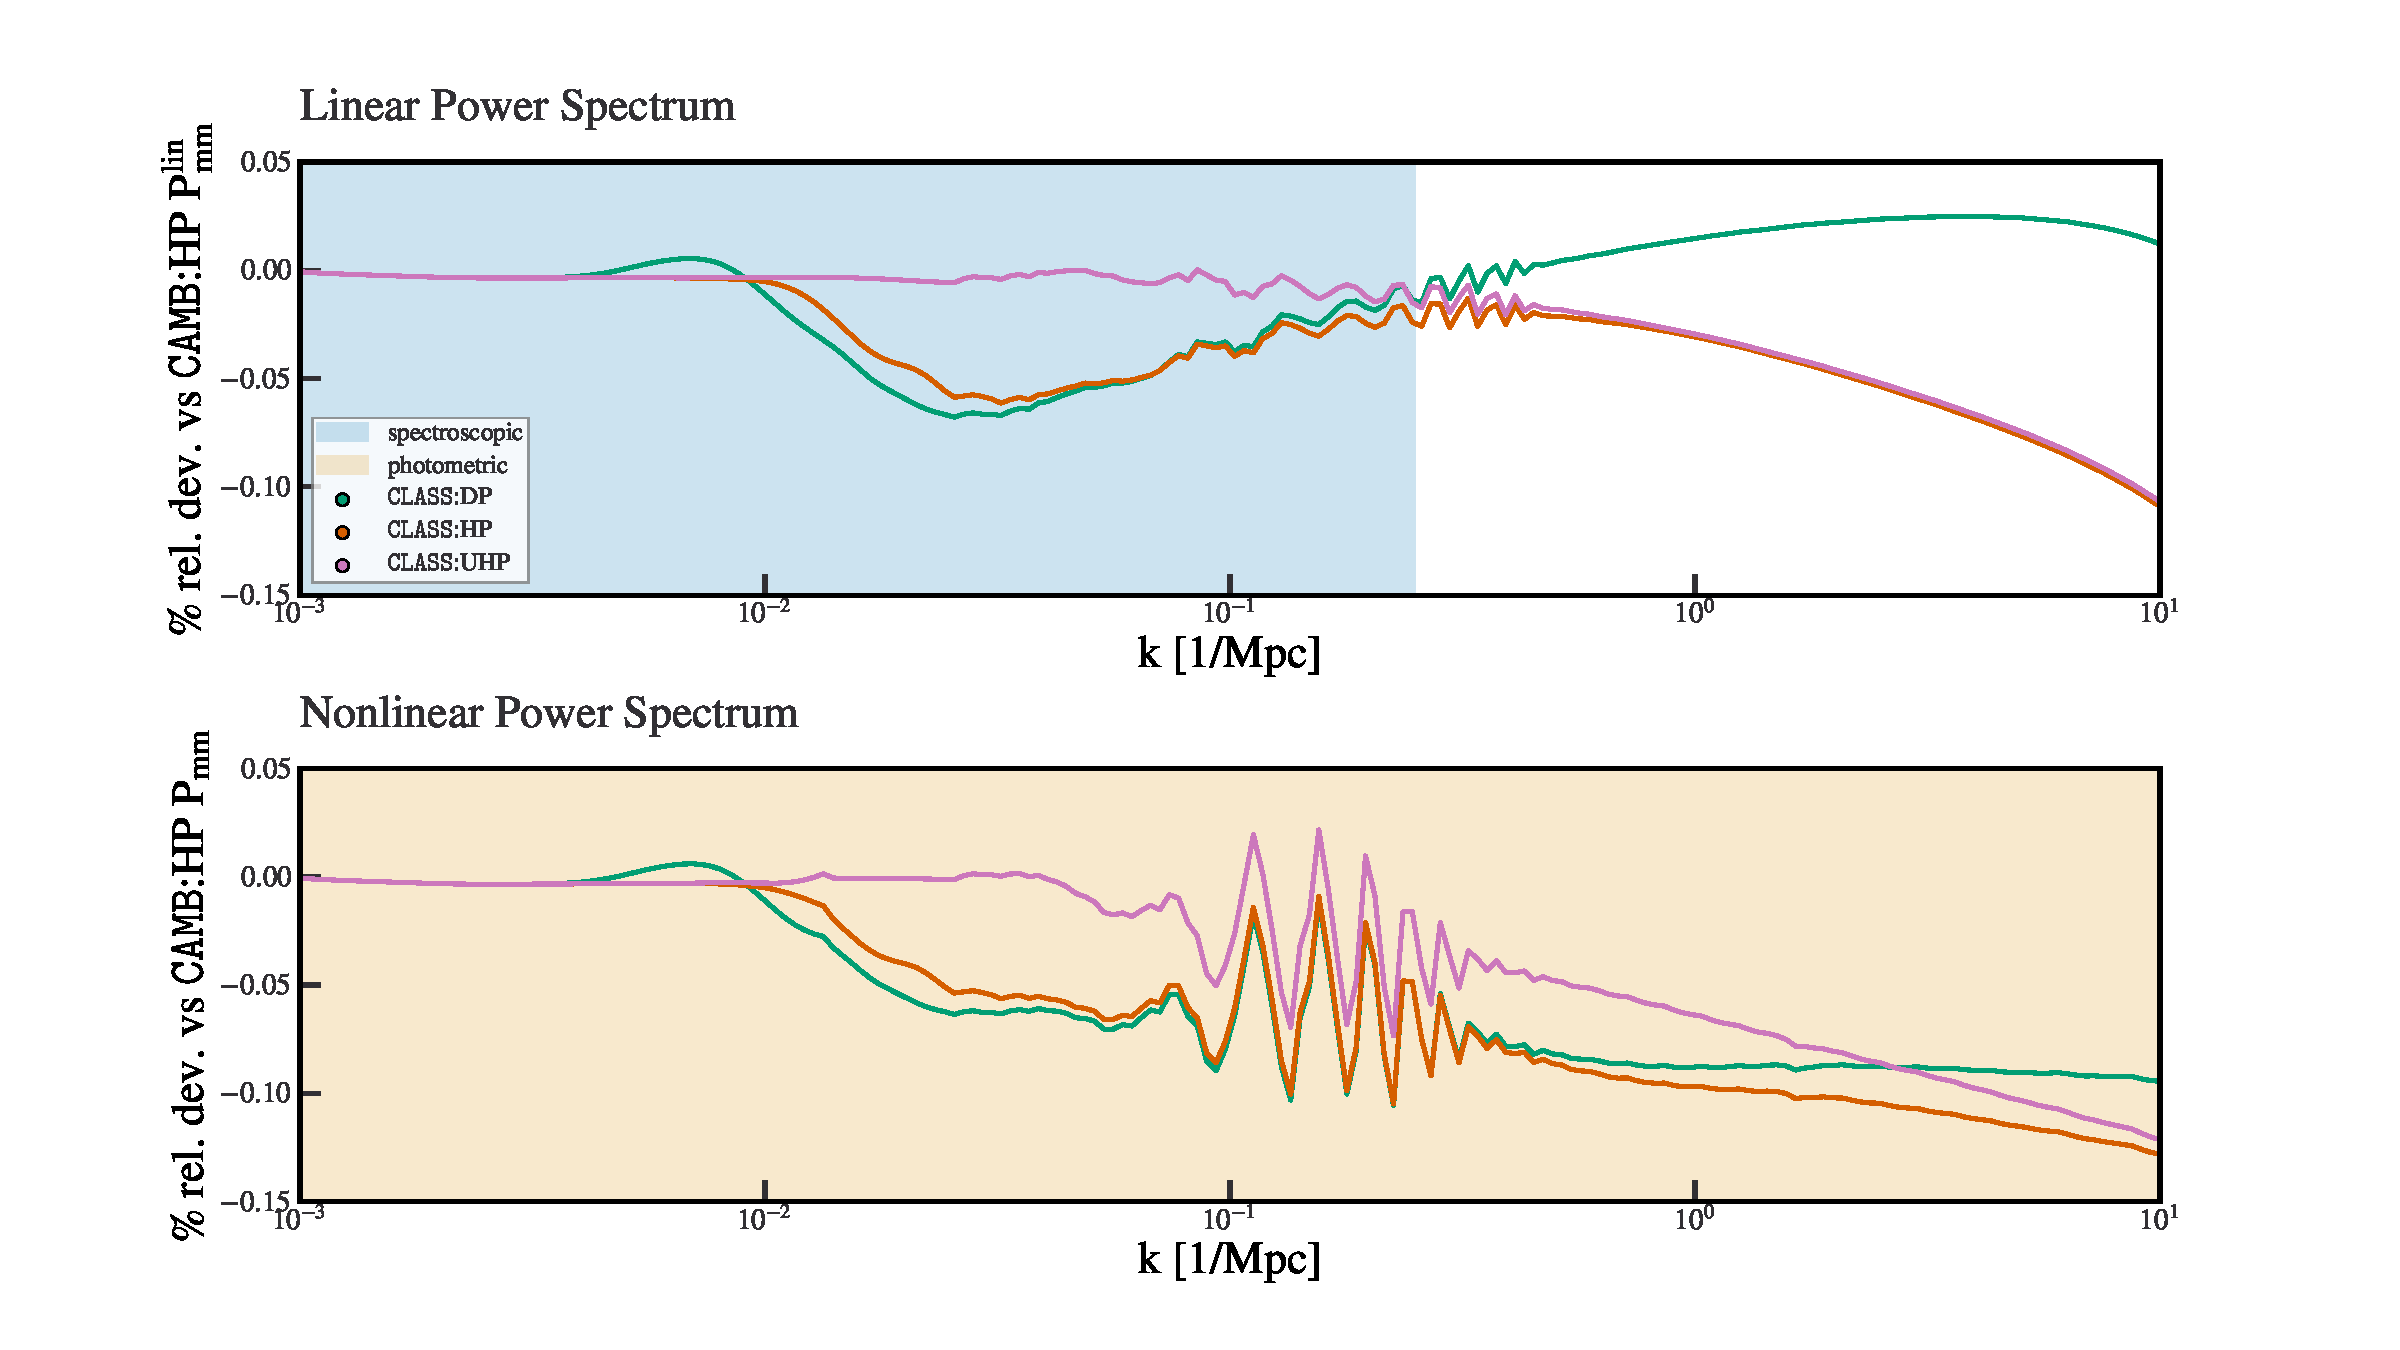
\includegraphics[width=0.9\linewidth]{../plots/../plots/Test_Precission_Parameter.pdf}
    \caption{Comparison of the different Class precision settings to our 'default' high precision setting for \camb. On the $y$ axis we plot the difference to the power spectra obtained from \camb, normalized to the mean value. We have marked the regions where the individual probes are sensitive to their corresponding colours.}
    \label{fig:precisson_settings}
 \end{figure}  
 For the linear power spectrum, we can see that the fluid approximation leads to an underprediction of 0.05\% on the matter power spectrum at intermediate $k$. At the smallest scales, it has a much smaller effect such that the \class:HP and \class:UHP settings agree very well with each other. What can also be seen, is that in the sensitivity region the power spectra of \class:HP and \class:DP only differ by a small bump at large scales, but then start diverging at small scales.\\
 For the nonlinear spectrum we can see a similar discrepancy between the different power spectra on large and intermediate scales, but then start converging again on the smallest scales, where the power spectra are dominated by the one halo term. We believe that the reason they start converging comes from the fact that the effective scalar index enters the smoothing region between one and two halo terms is slightly different. This can be explained by the fact that we observe a stronger neutrino-induced suppression on intermediate scales when doing the fluid approximation.\\
\section{Comparison of the different Fisher Information Methods}
\begin{figure}
    \centering
    \caption{Comparisons of the one-dimensional marginalized (in light grey) and unmarginalized errors (in dark grey). The \Euclid probe is the spectroscopic probe with the optimistic settings. We use the abbreviation $lbs_i$ stands for the nuisance parameter $\ln(\hat{b}\sigma_8)_i$, where $i$ denotes the redshift bin. We plot the percentage deviation from the median error obtained by \cosmicfish:\camb. }
    \begin{subfigure}[b]{0.49\textwidth}
        \centering
        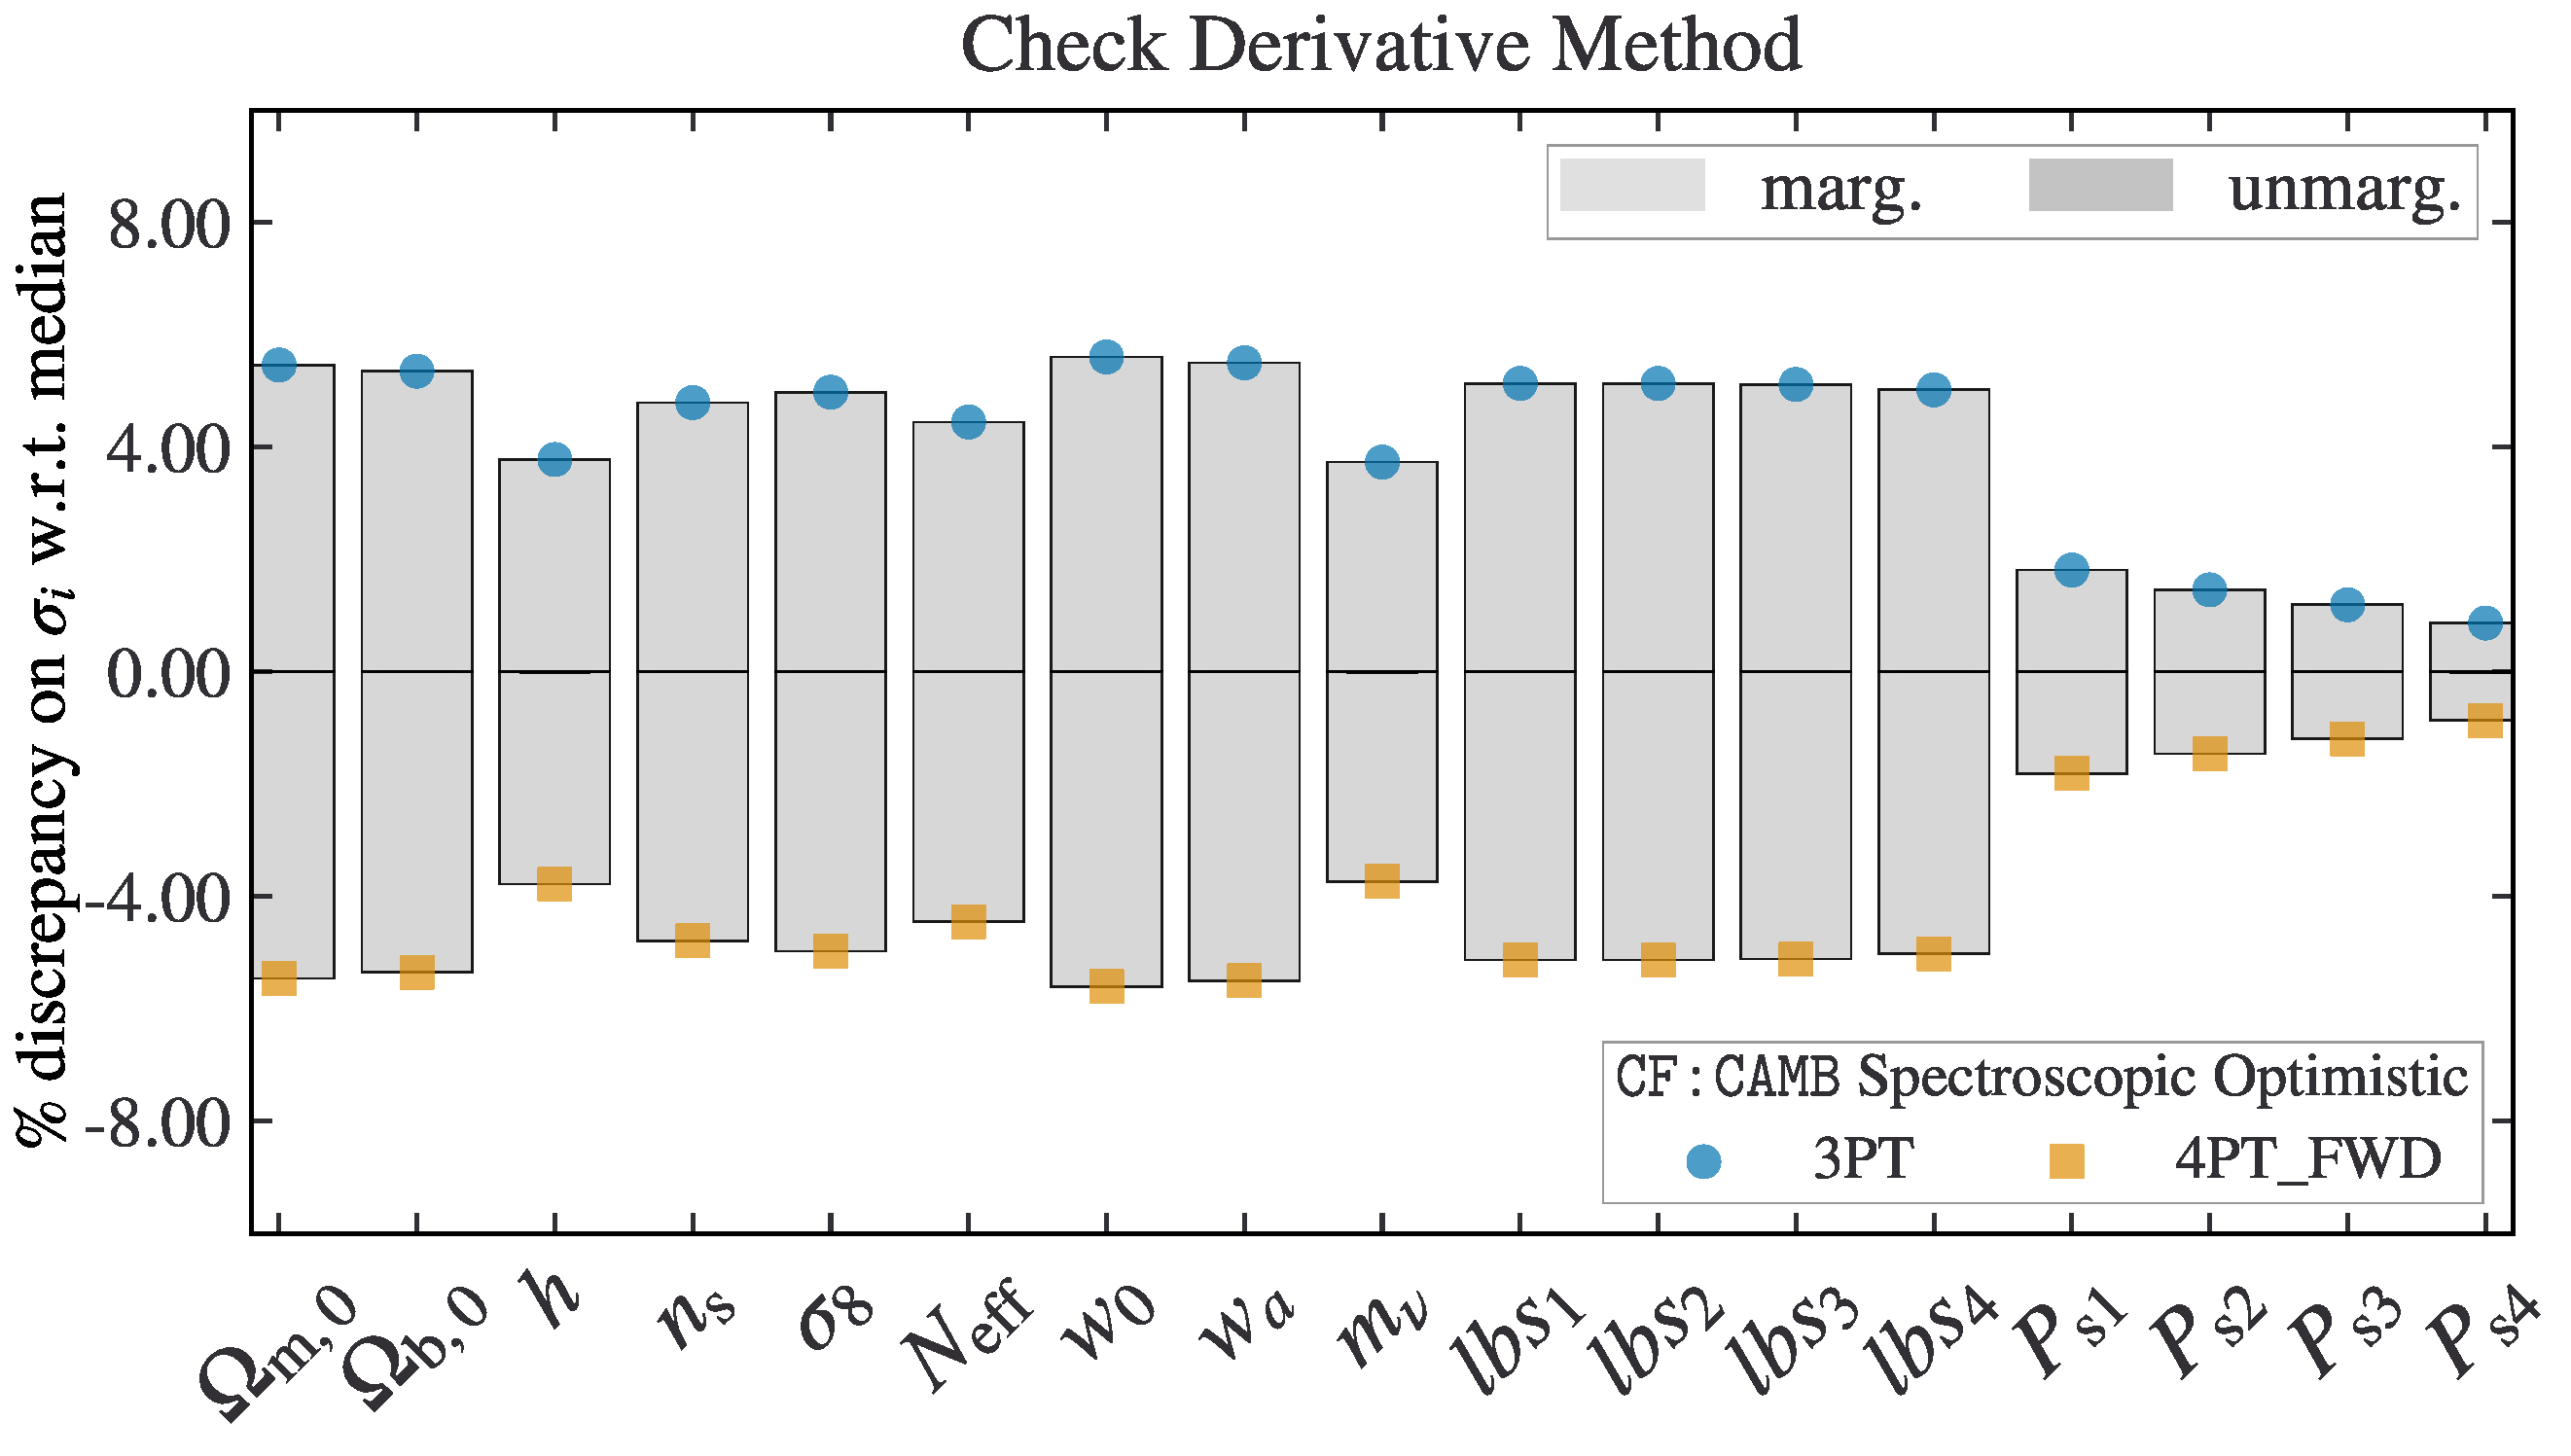
\includegraphics[width=\textwidth]{../plots/Test_Derivative_Method.pdf}
        \caption{Comparison of the errors when switching the derivative method}
        \label{fig:comparison_derivs}
    \end{subfigure}
    \hfill
    \begin{subfigure}[b]{0.49\textwidth}
        \centering
        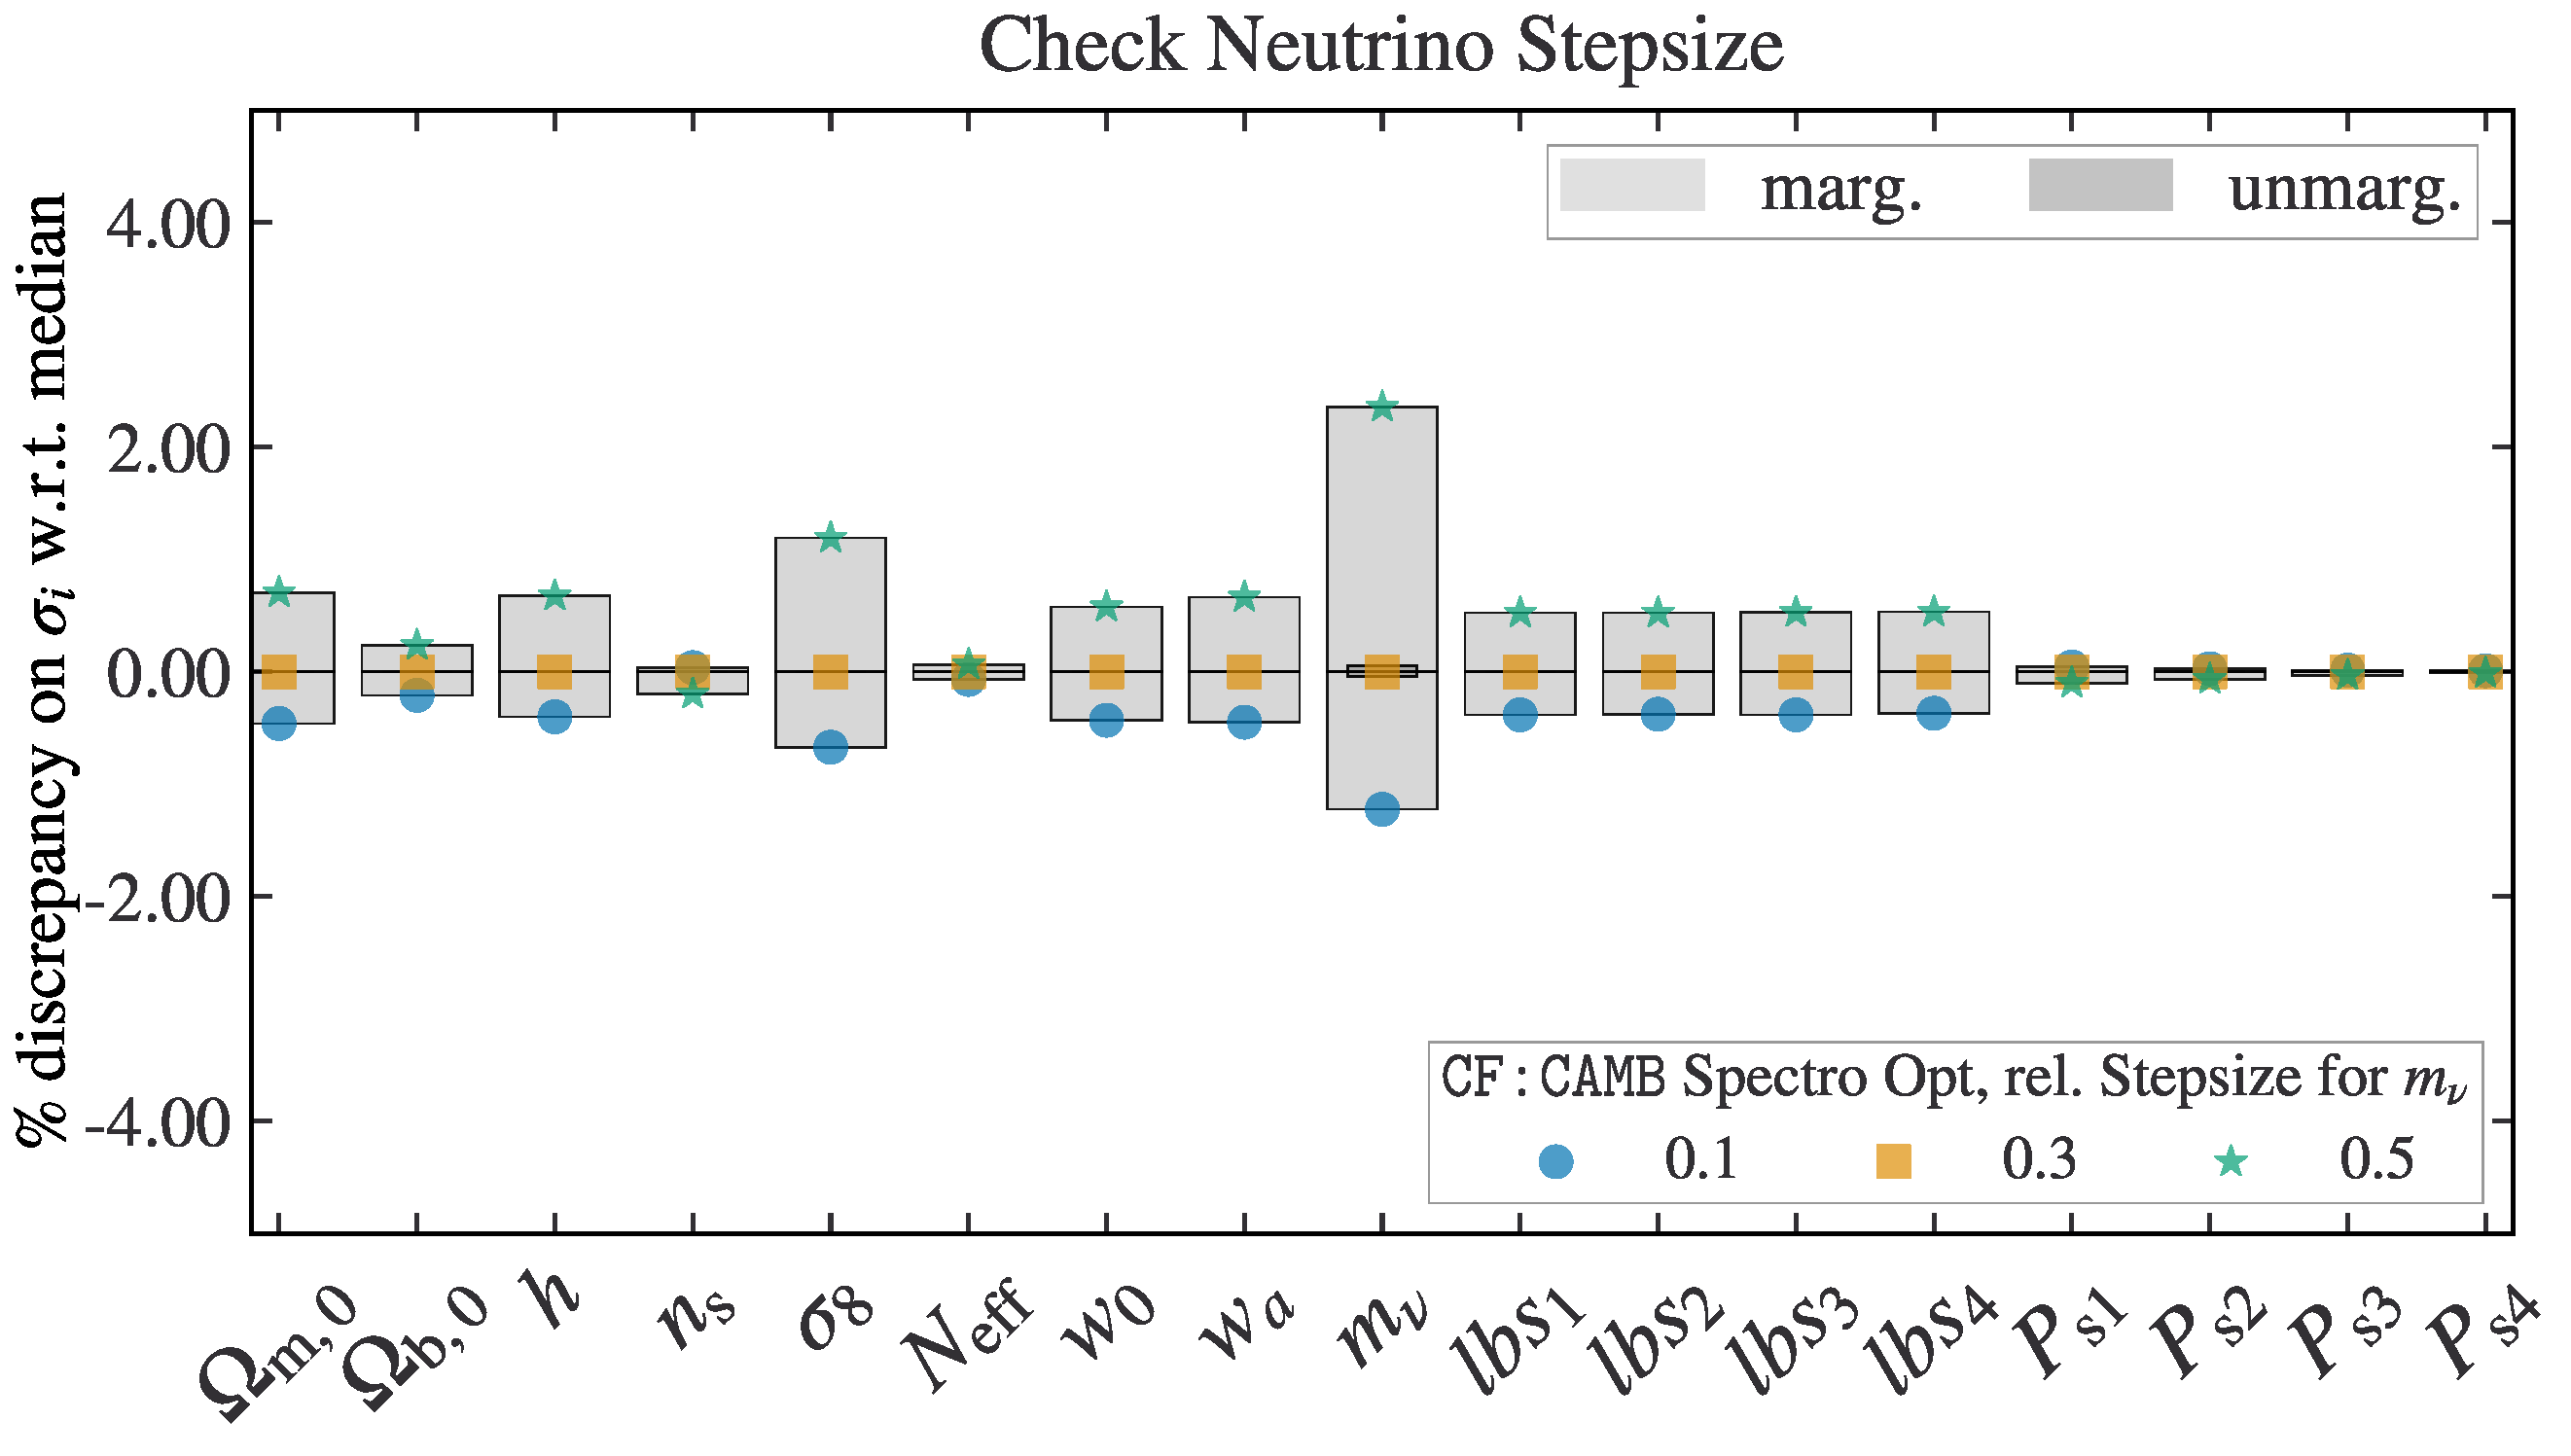
\includegraphics[width=\textwidth]{../plots/Test_mnu_Stepsize.pdf}
        \caption{Comparison of the errors when changing the relative stepsize for the neutrino mass.}
        \label{fig:comparasion_mnu_stepsize}  
    \end{subfigure}
       \label{fig:deriv_tests} 
\end{figure}
\begin{figure}
    \centering
    \caption{In this figure we compare the results from \cosmicfish using either of the  two different Einstein Boltzmann solvers and MontePython in fisher mode, denoted with {\tt MP:Fisher}.}
    \begin{subfigure}[b]{0.49\textwidth}
        \centering
        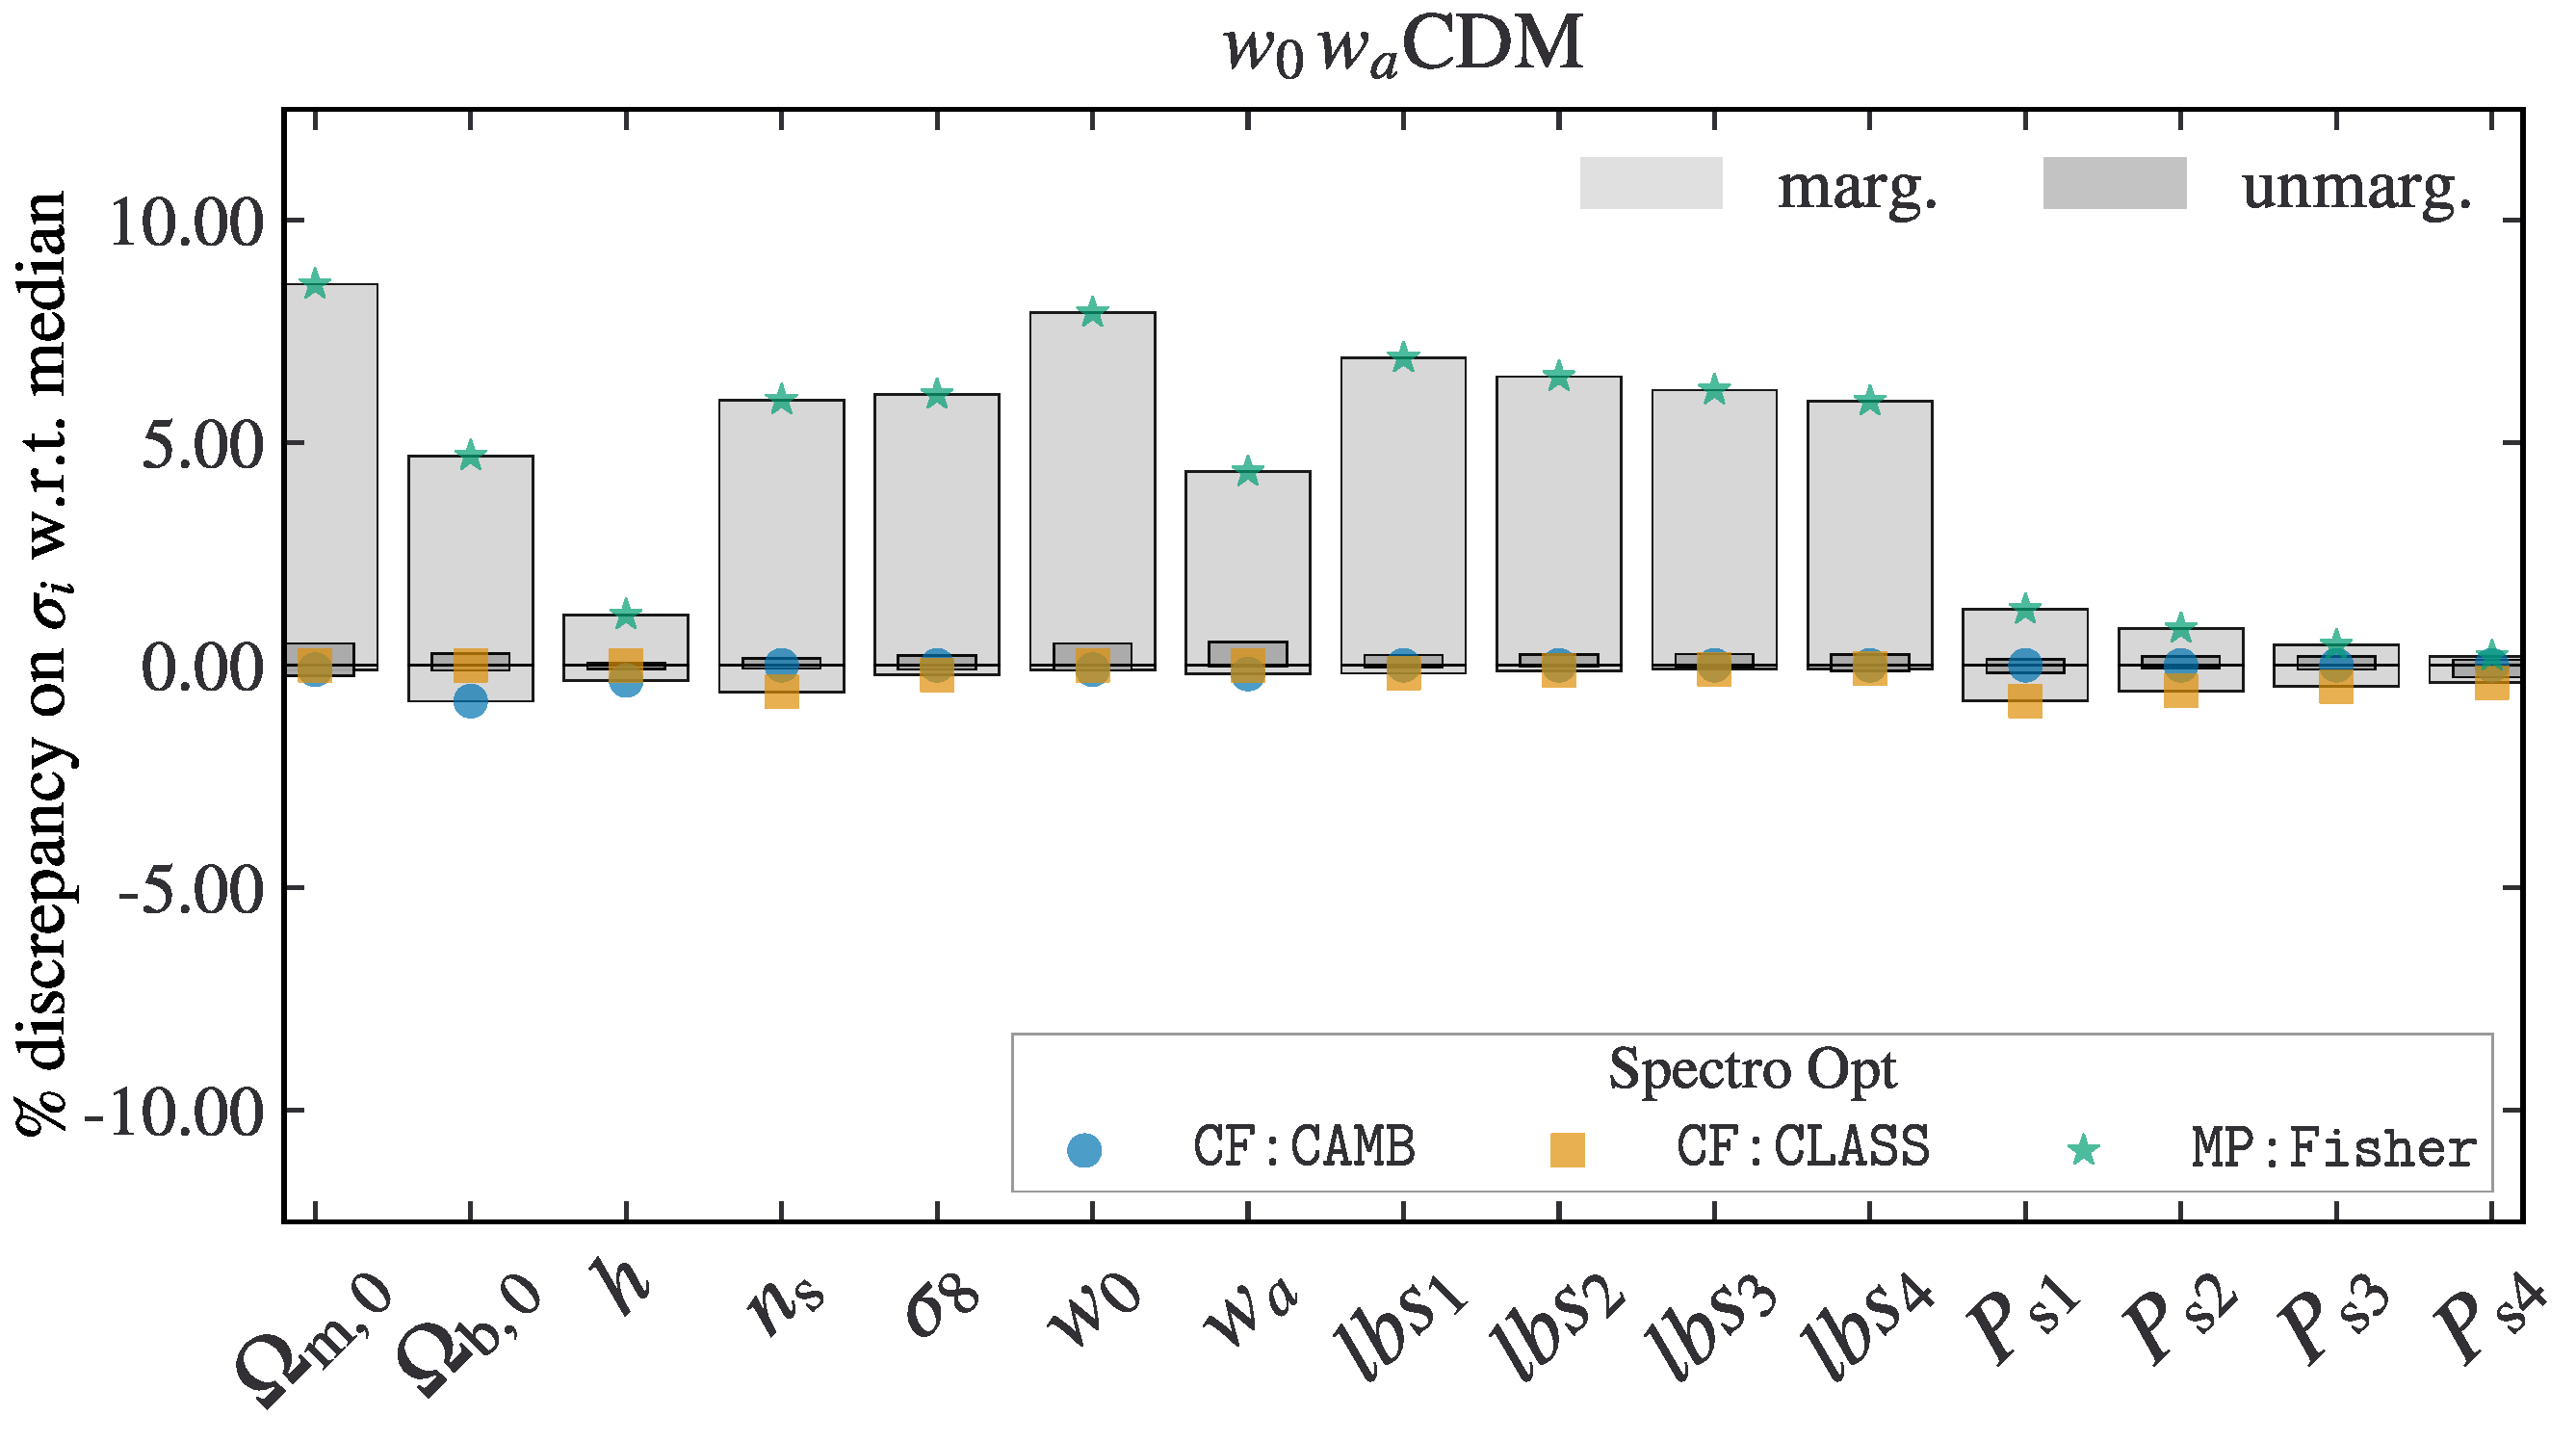
\includegraphics[width=\textwidth]{../plots/Spectro_Opt_wCDM_error_comparison.pdf}
        \caption{the spectroscopic optimistic probe}
        \label{fig:w0wa_1}
    \end{subfigure}
    \hfill
    \begin{subfigure}[b]{0.49\textwidth}
        \centering
        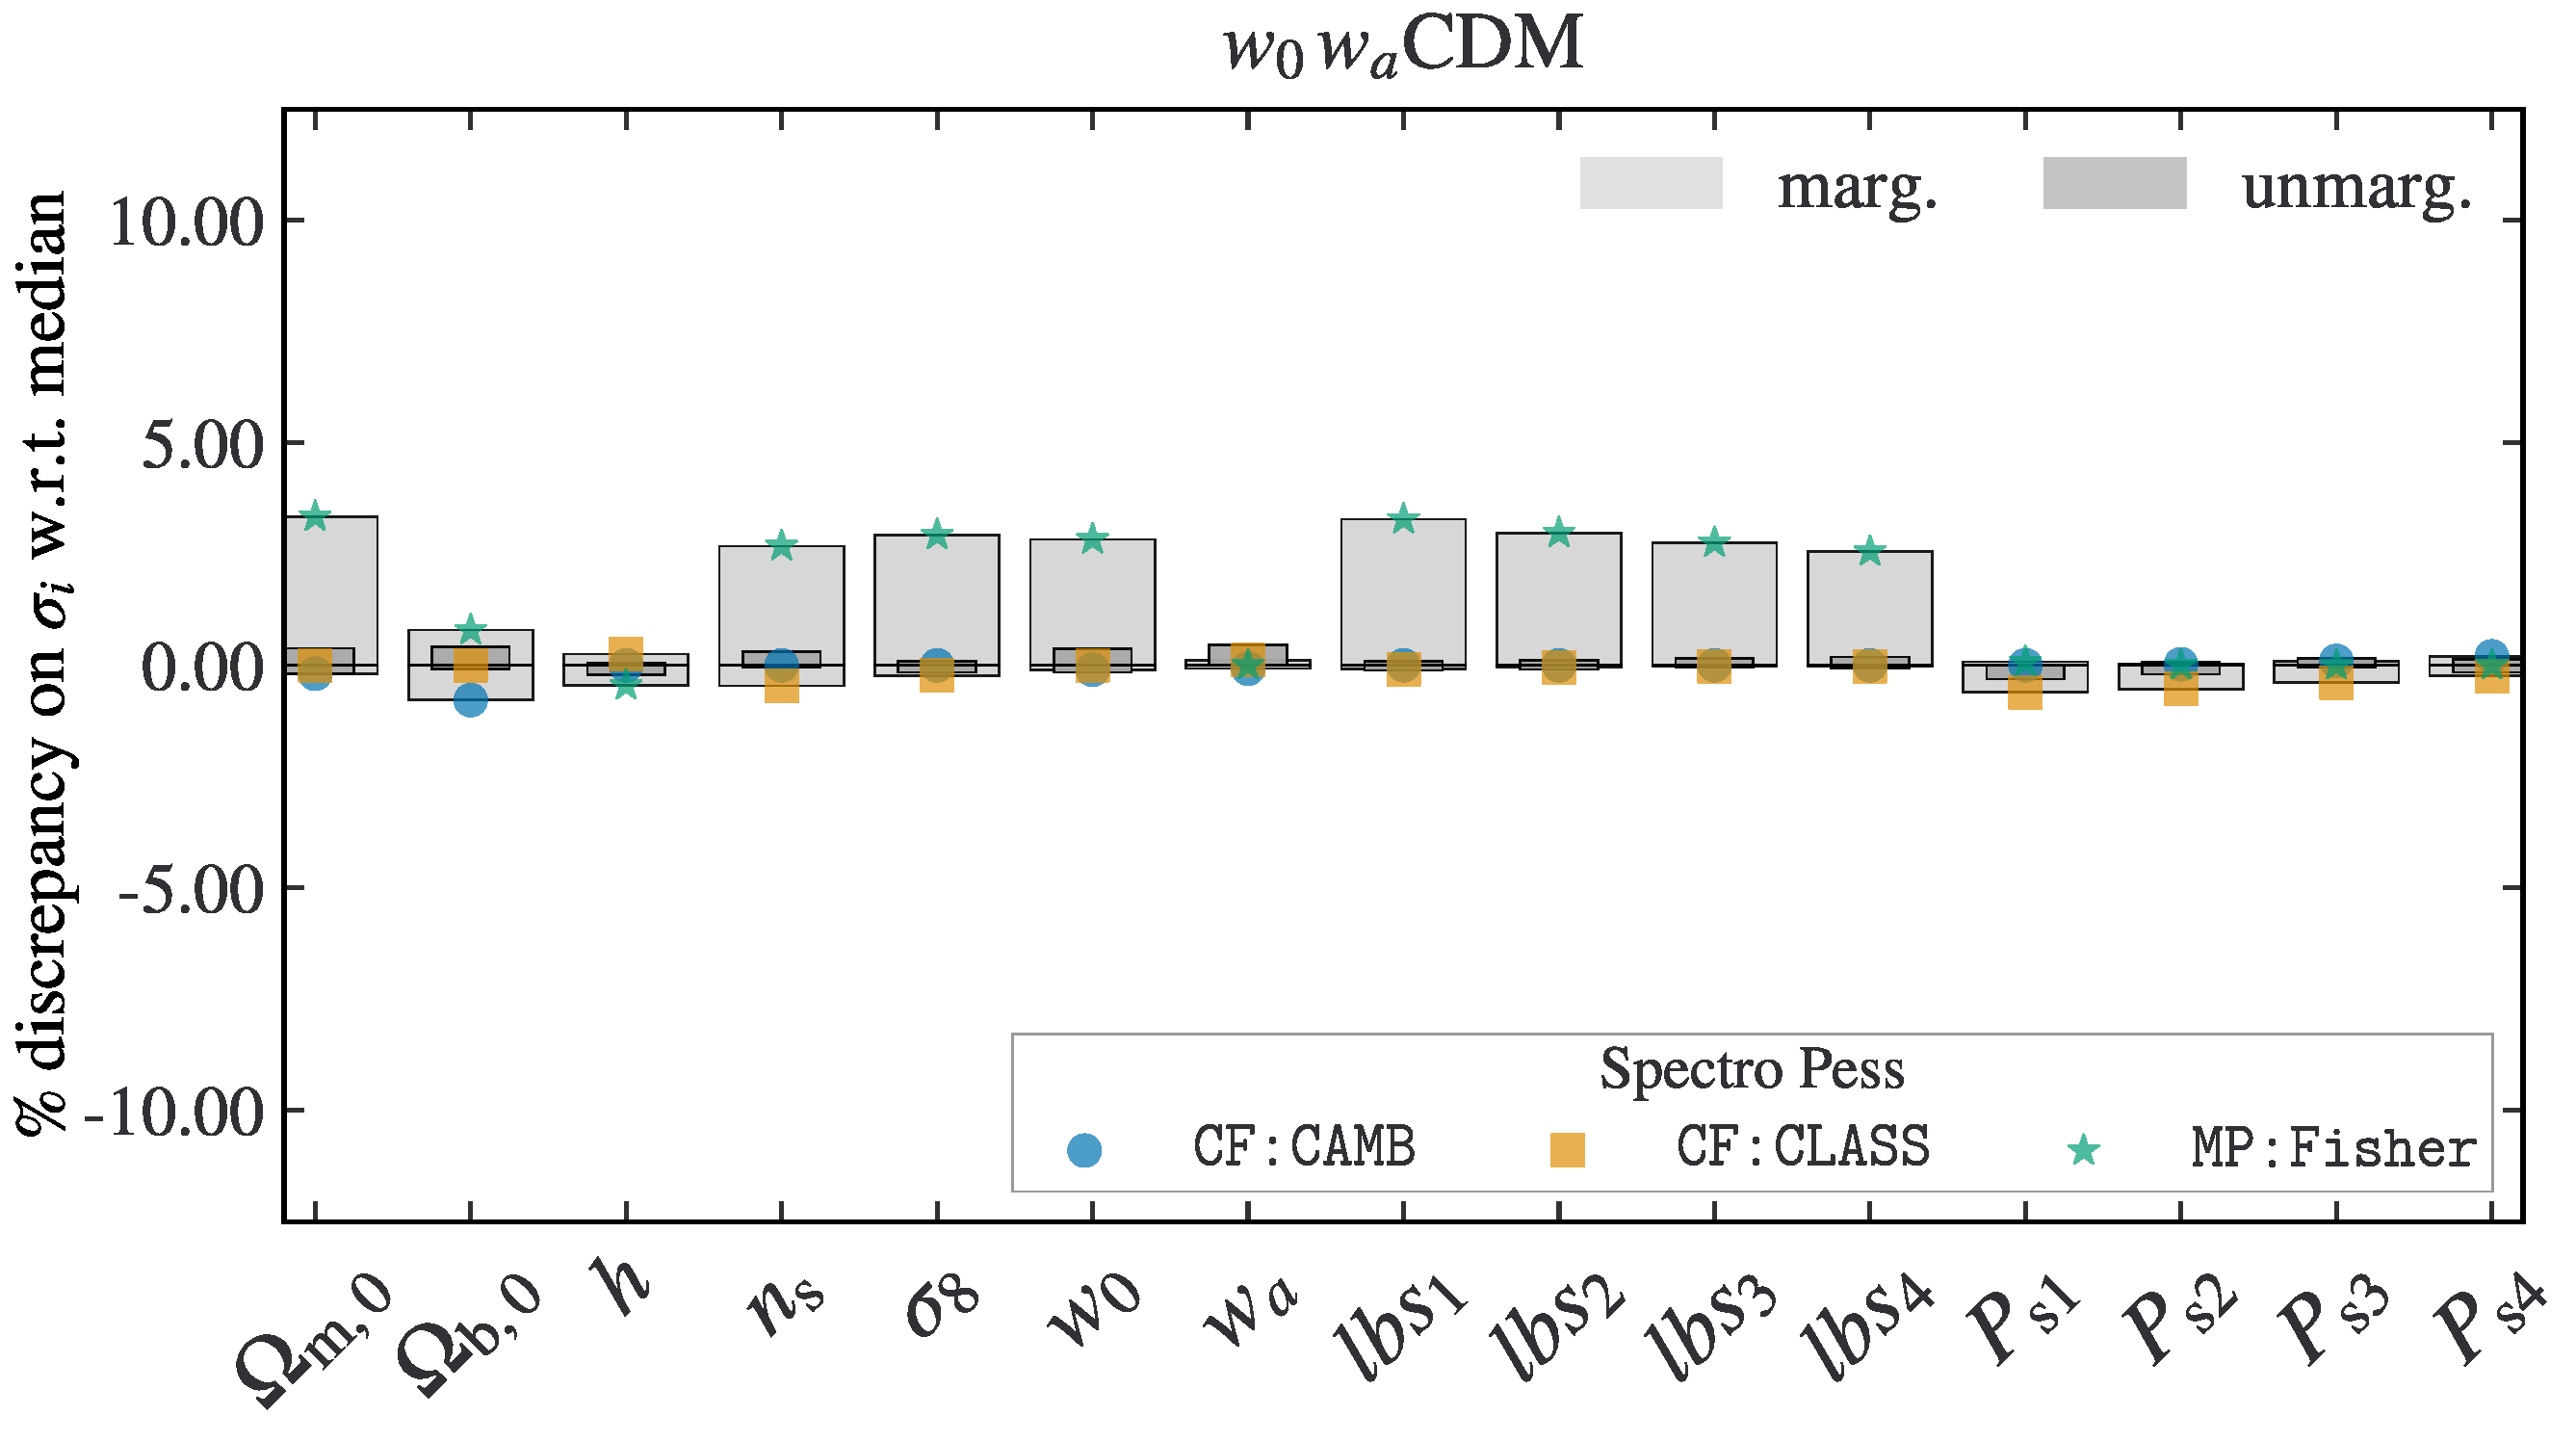
\includegraphics[width=\textwidth]{../plots/Spectro_Pess_wCDM_error_comparison.pdf}
        \caption{the spectroscopic pessimistic probe}
        \label{fig:w0wa_2}  
    \end{subfigure}\\
    \begin{subfigure}[b]{0.49\textwidth}
        \centering
        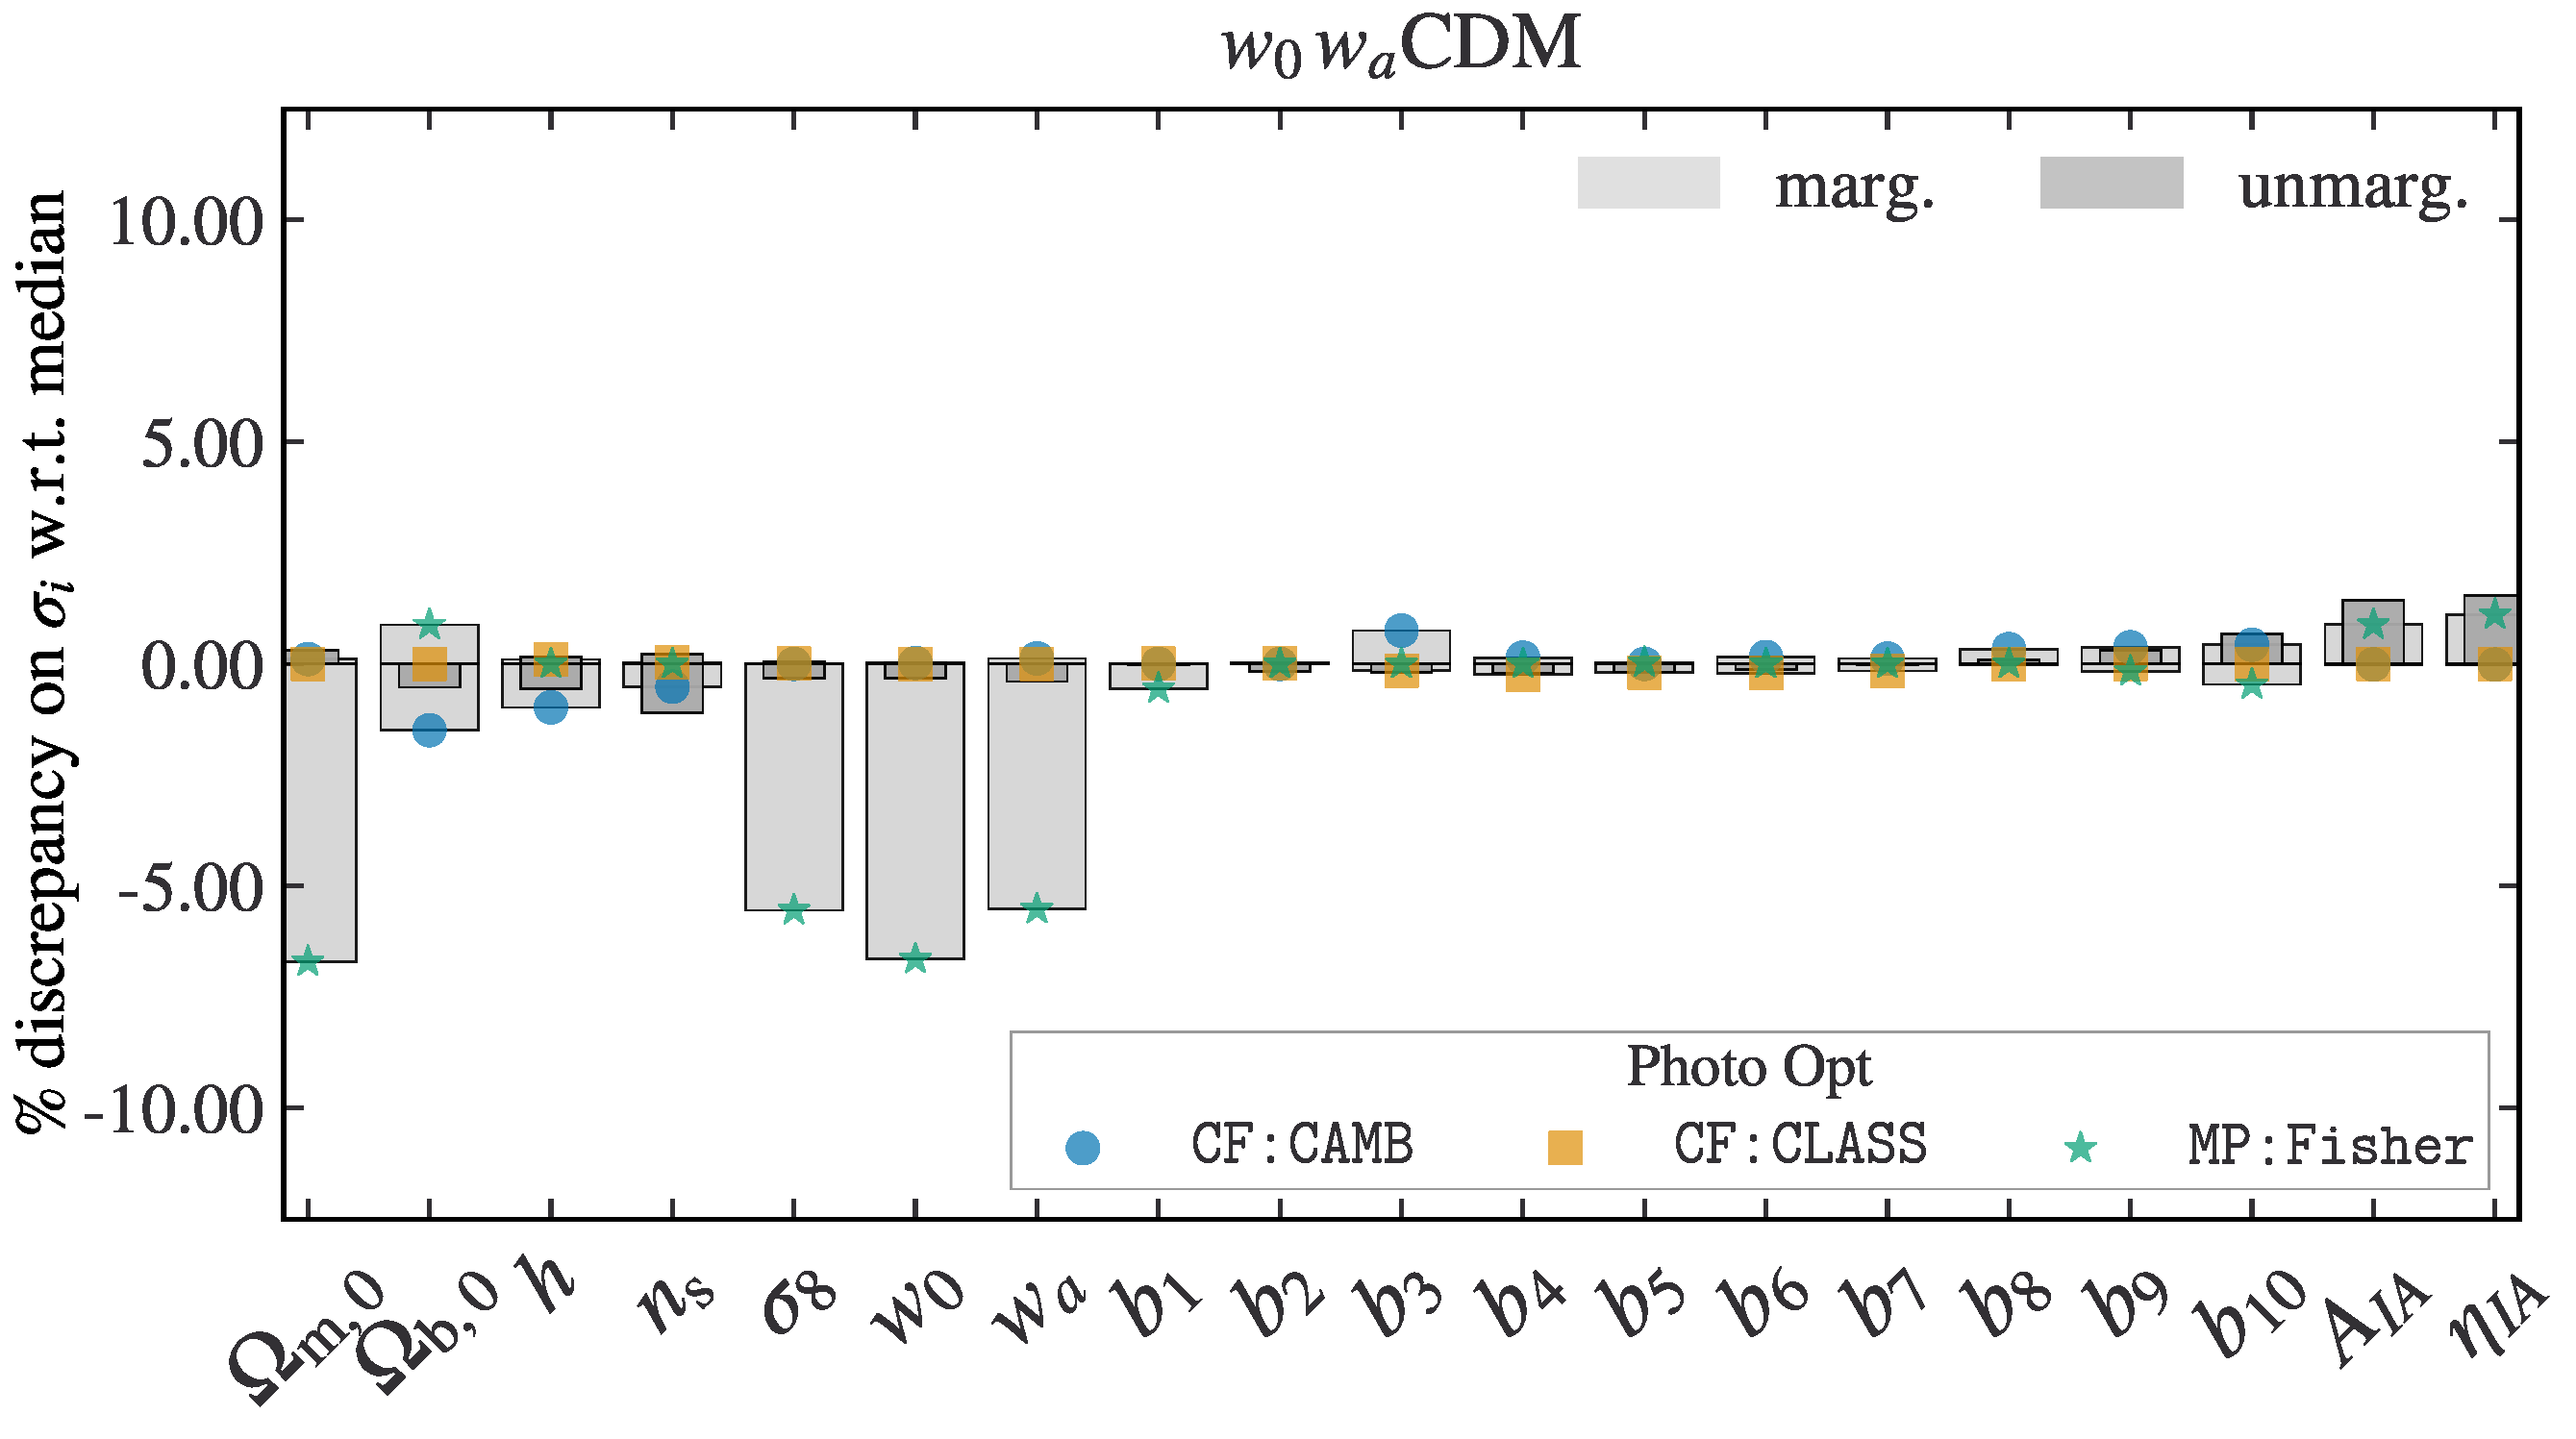
\includegraphics[width=\textwidth]{../plots/Photo_Opt_wCDM_error_comparison.pdf}
        \caption{the photometric optimistic probe}
        \label{fig:w0wa_3}
    \end{subfigure}
    \hfill
    \begin{subfigure}[b]{0.49\textwidth}
        \centering
        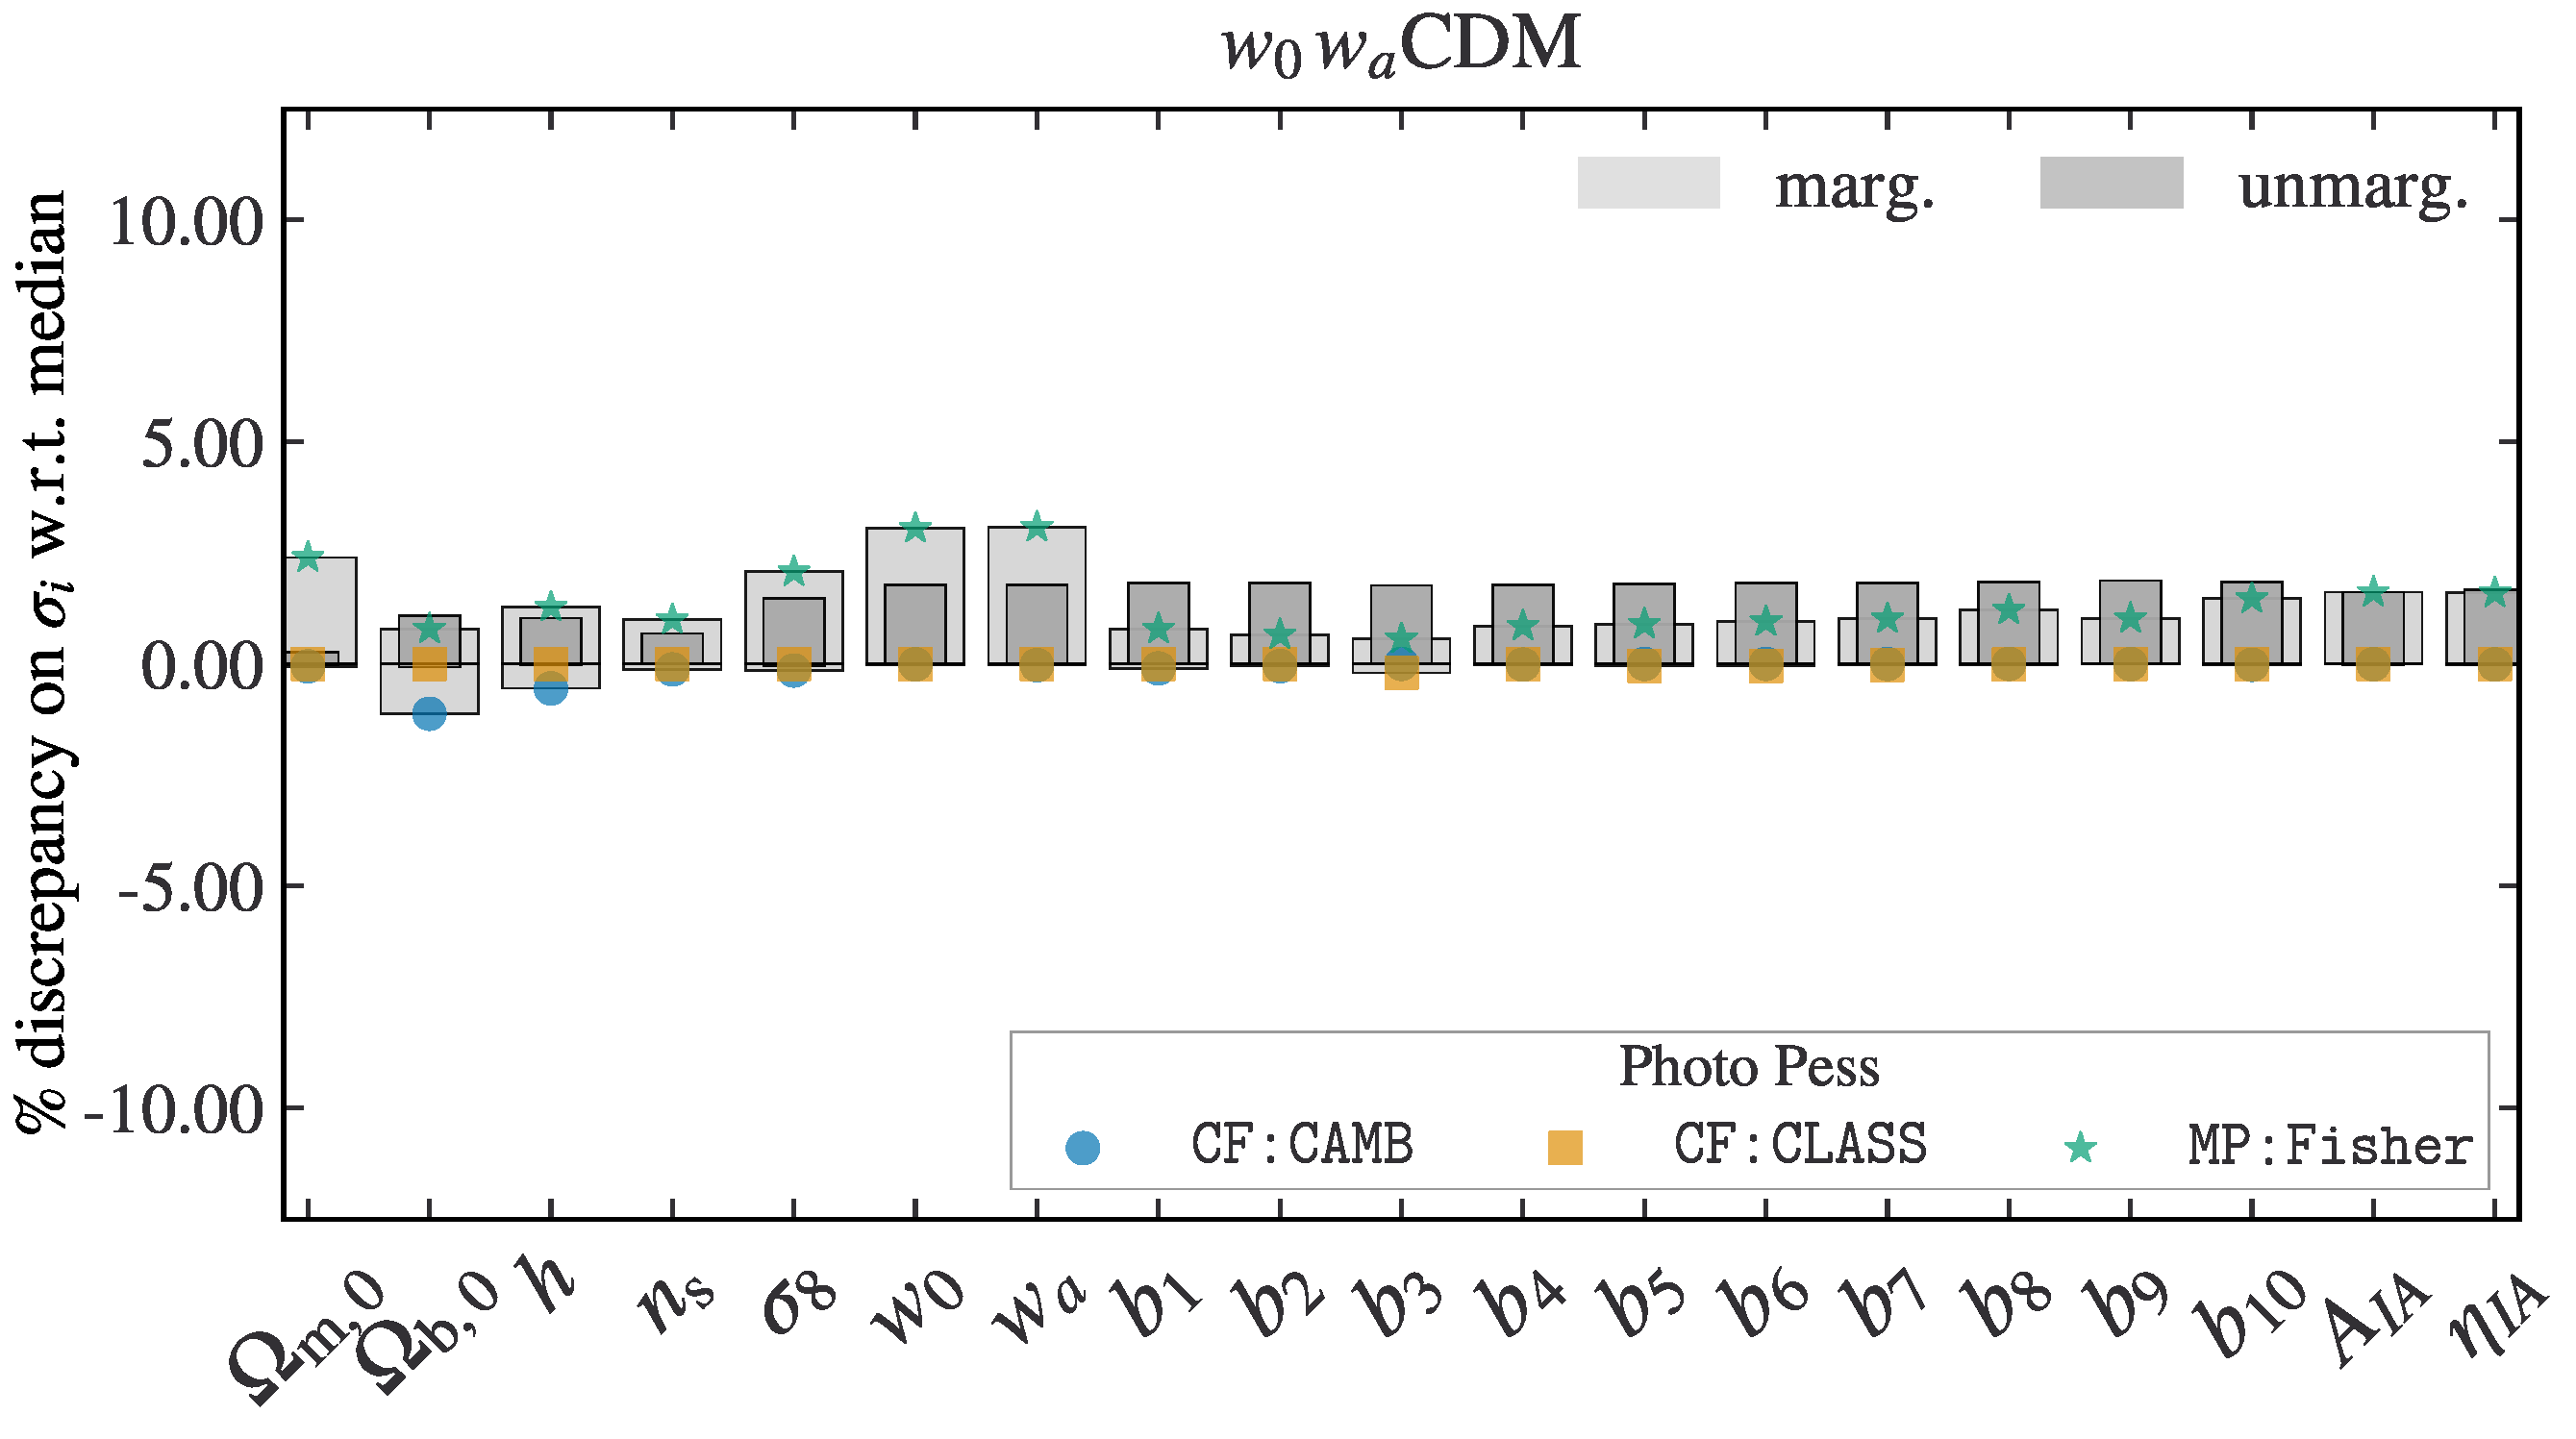
\includegraphics[width=\textwidth]{../plots/Photo_Pess_wCDM_error_comparison.pdf}
        \caption{the photometric pessimistic probe}
        \label{fig:w0wa_4}  
    \end{subfigure}    
       \label{fig:Comparison_w0wa} 
\end{figure}
\begin{figure}
    \centering
    \caption{Same as figure \ref{fig:Comparison_w0wa} but for the $w_0$CDM+$m_\nu$ model}
    \begin{subfigure}[b]{0.49\textwidth}
        \centering
        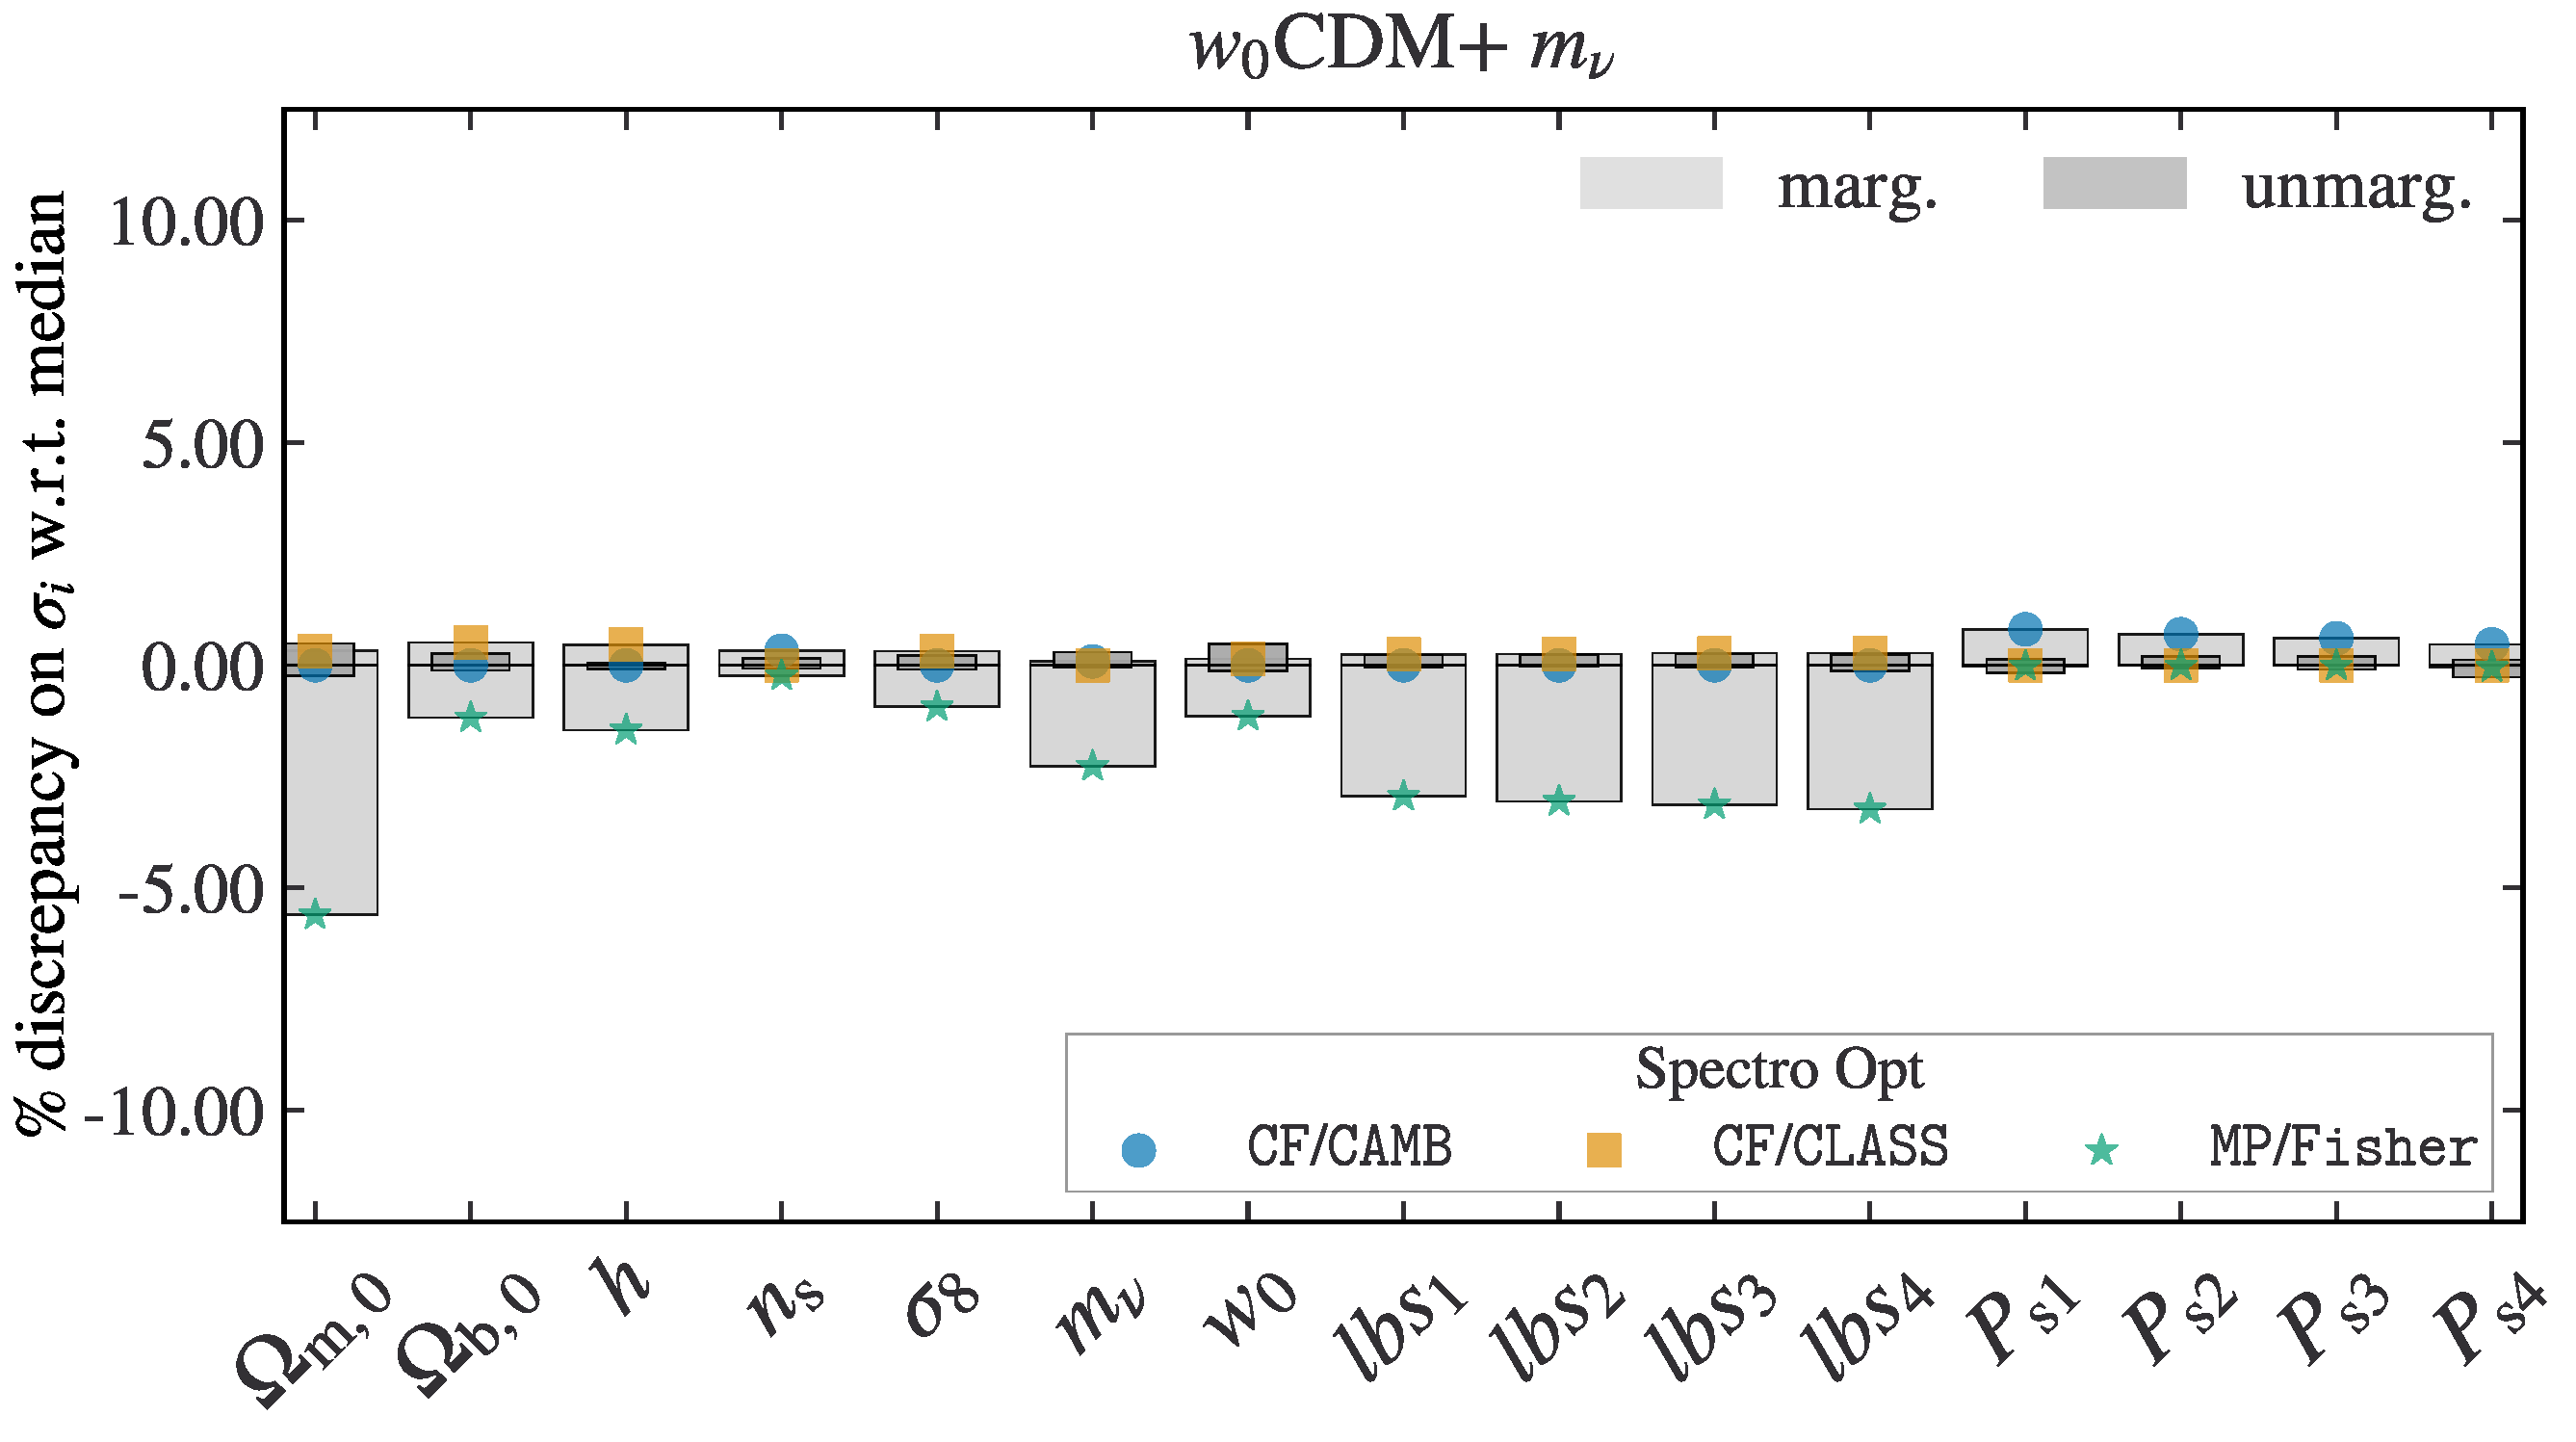
\includegraphics[width=\textwidth]{../plots/Spectro_Opt_mnu+w0_error_comparison.pdf}
    \end{subfigure}
    \hfill
    \begin{subfigure}[b]{0.49\textwidth}
        \centering
        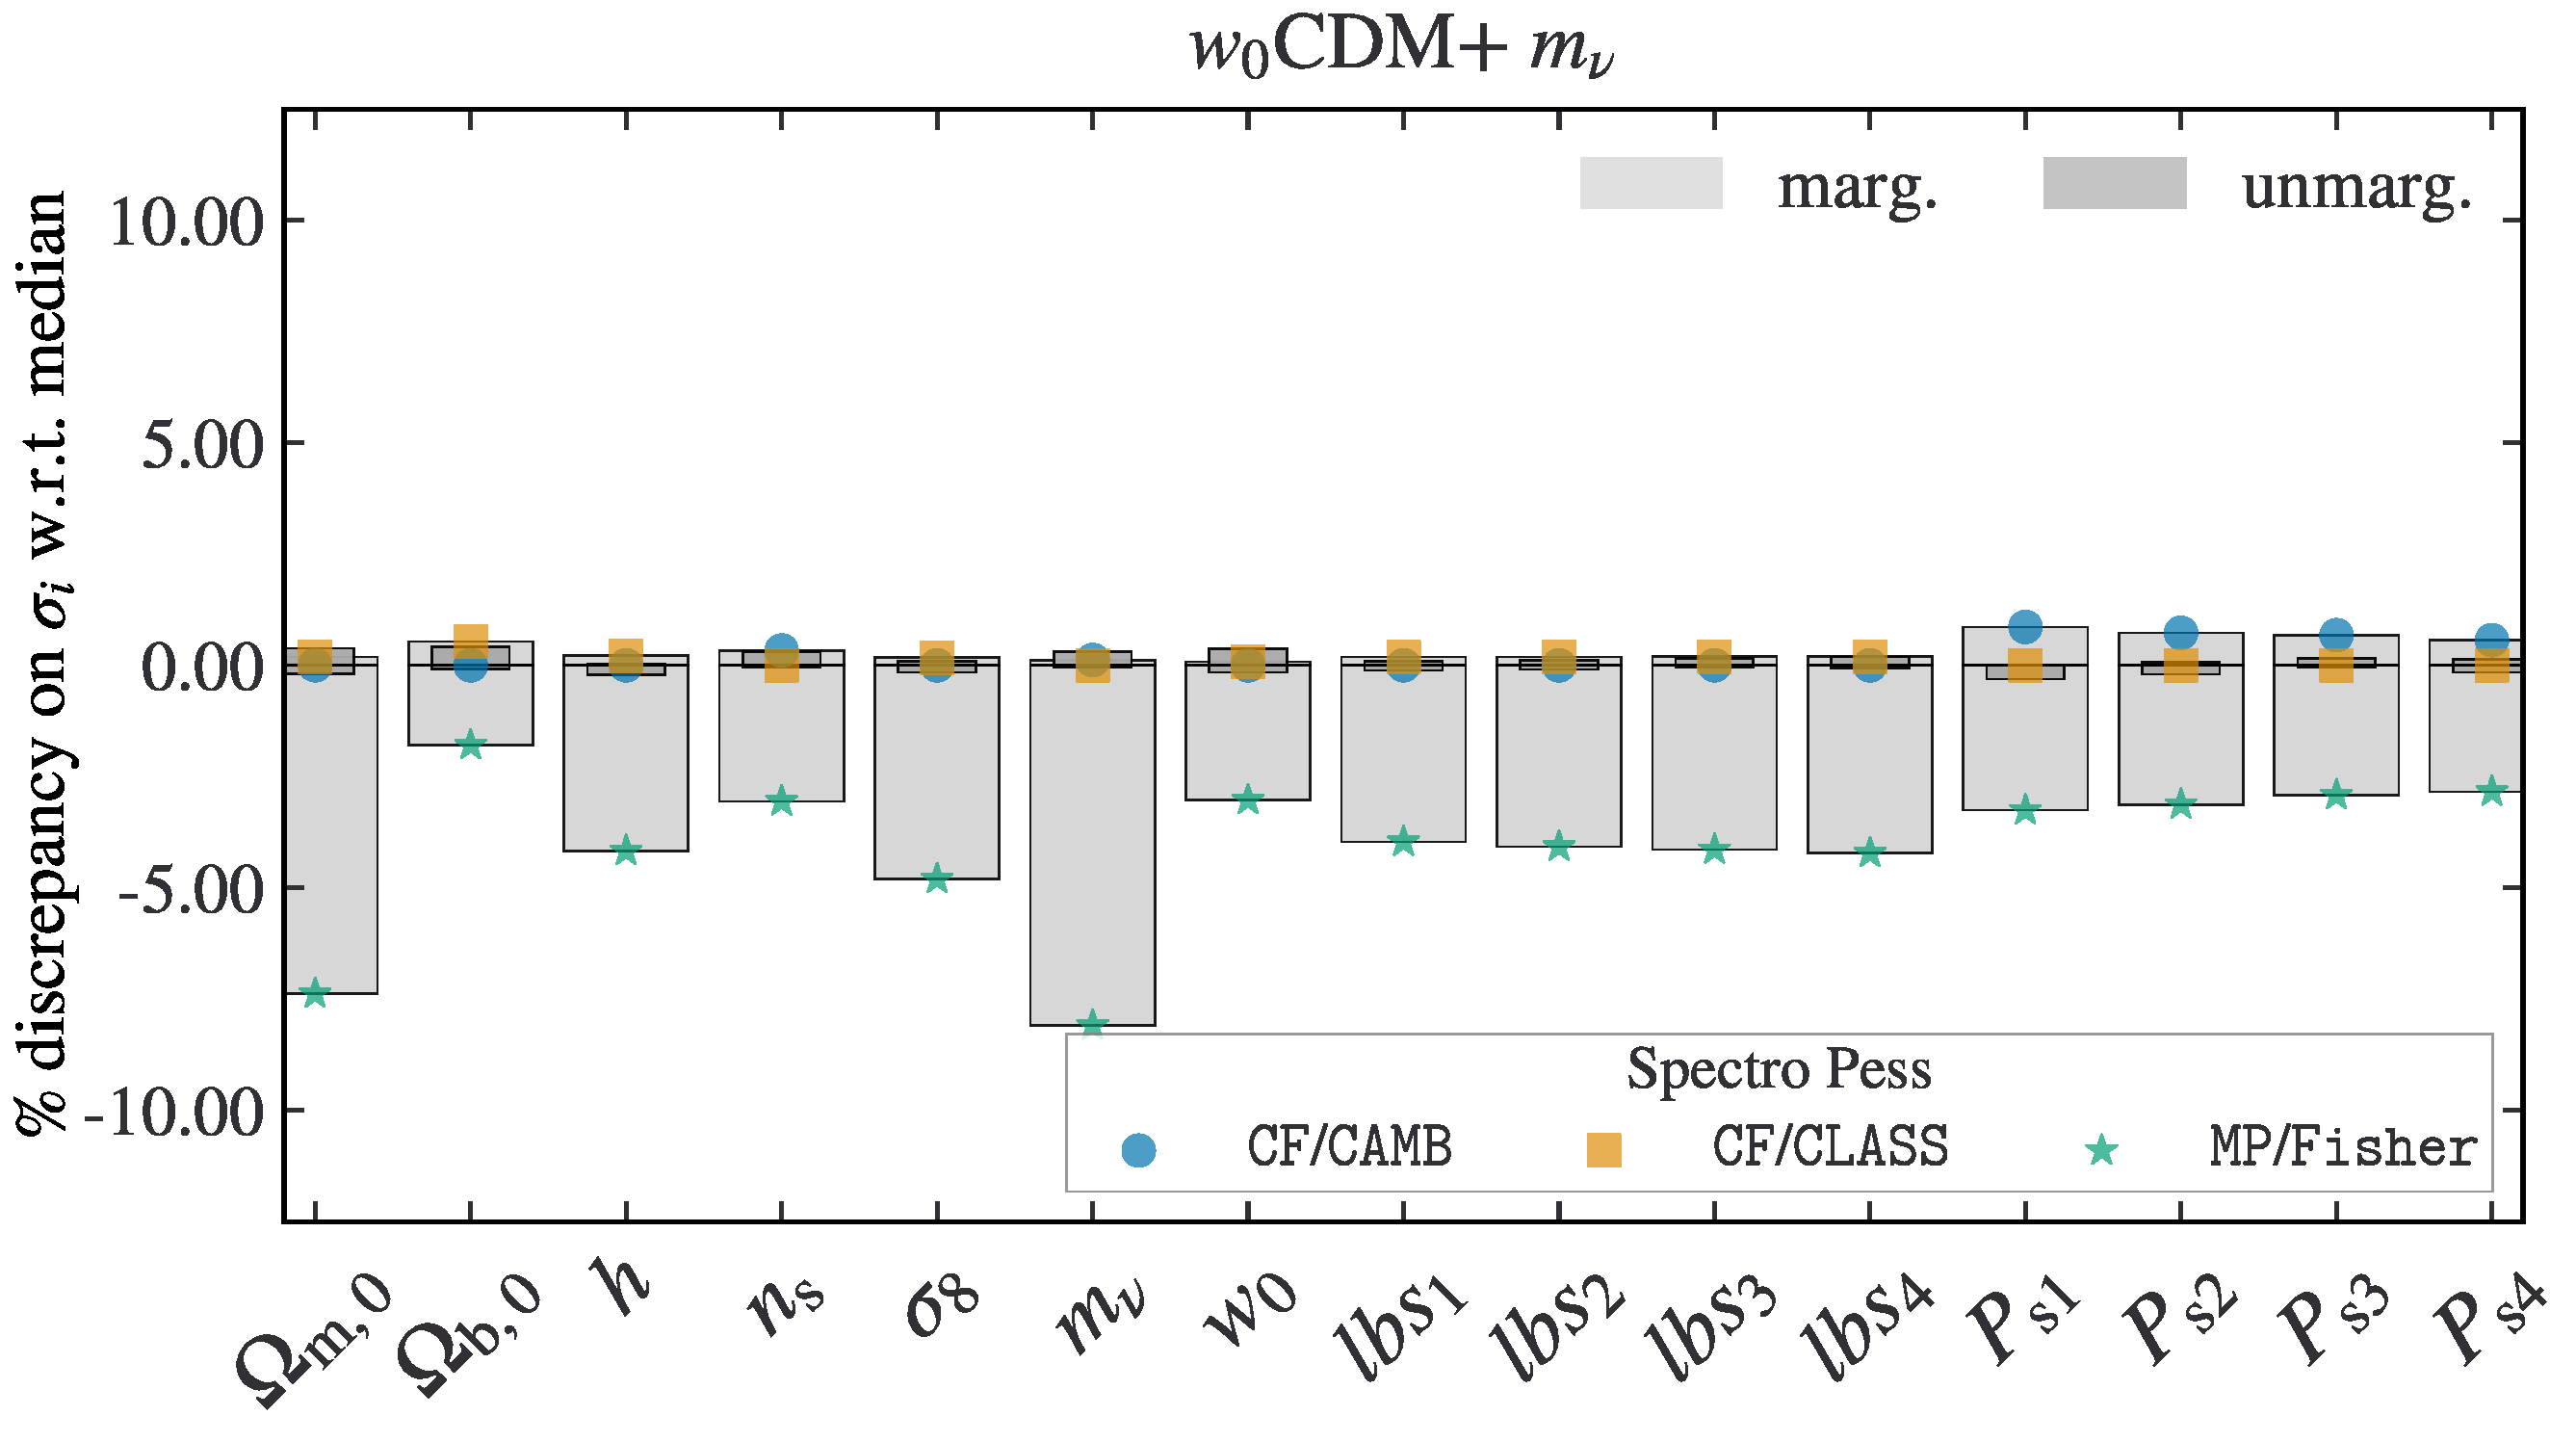
\includegraphics[width=\textwidth]{../plots/Spectro_Pess_mnu+w0_error_comparison.pdf}
    \end{subfigure}\\
    \begin{subfigure}[b]{0.49\textwidth}
        \centering
        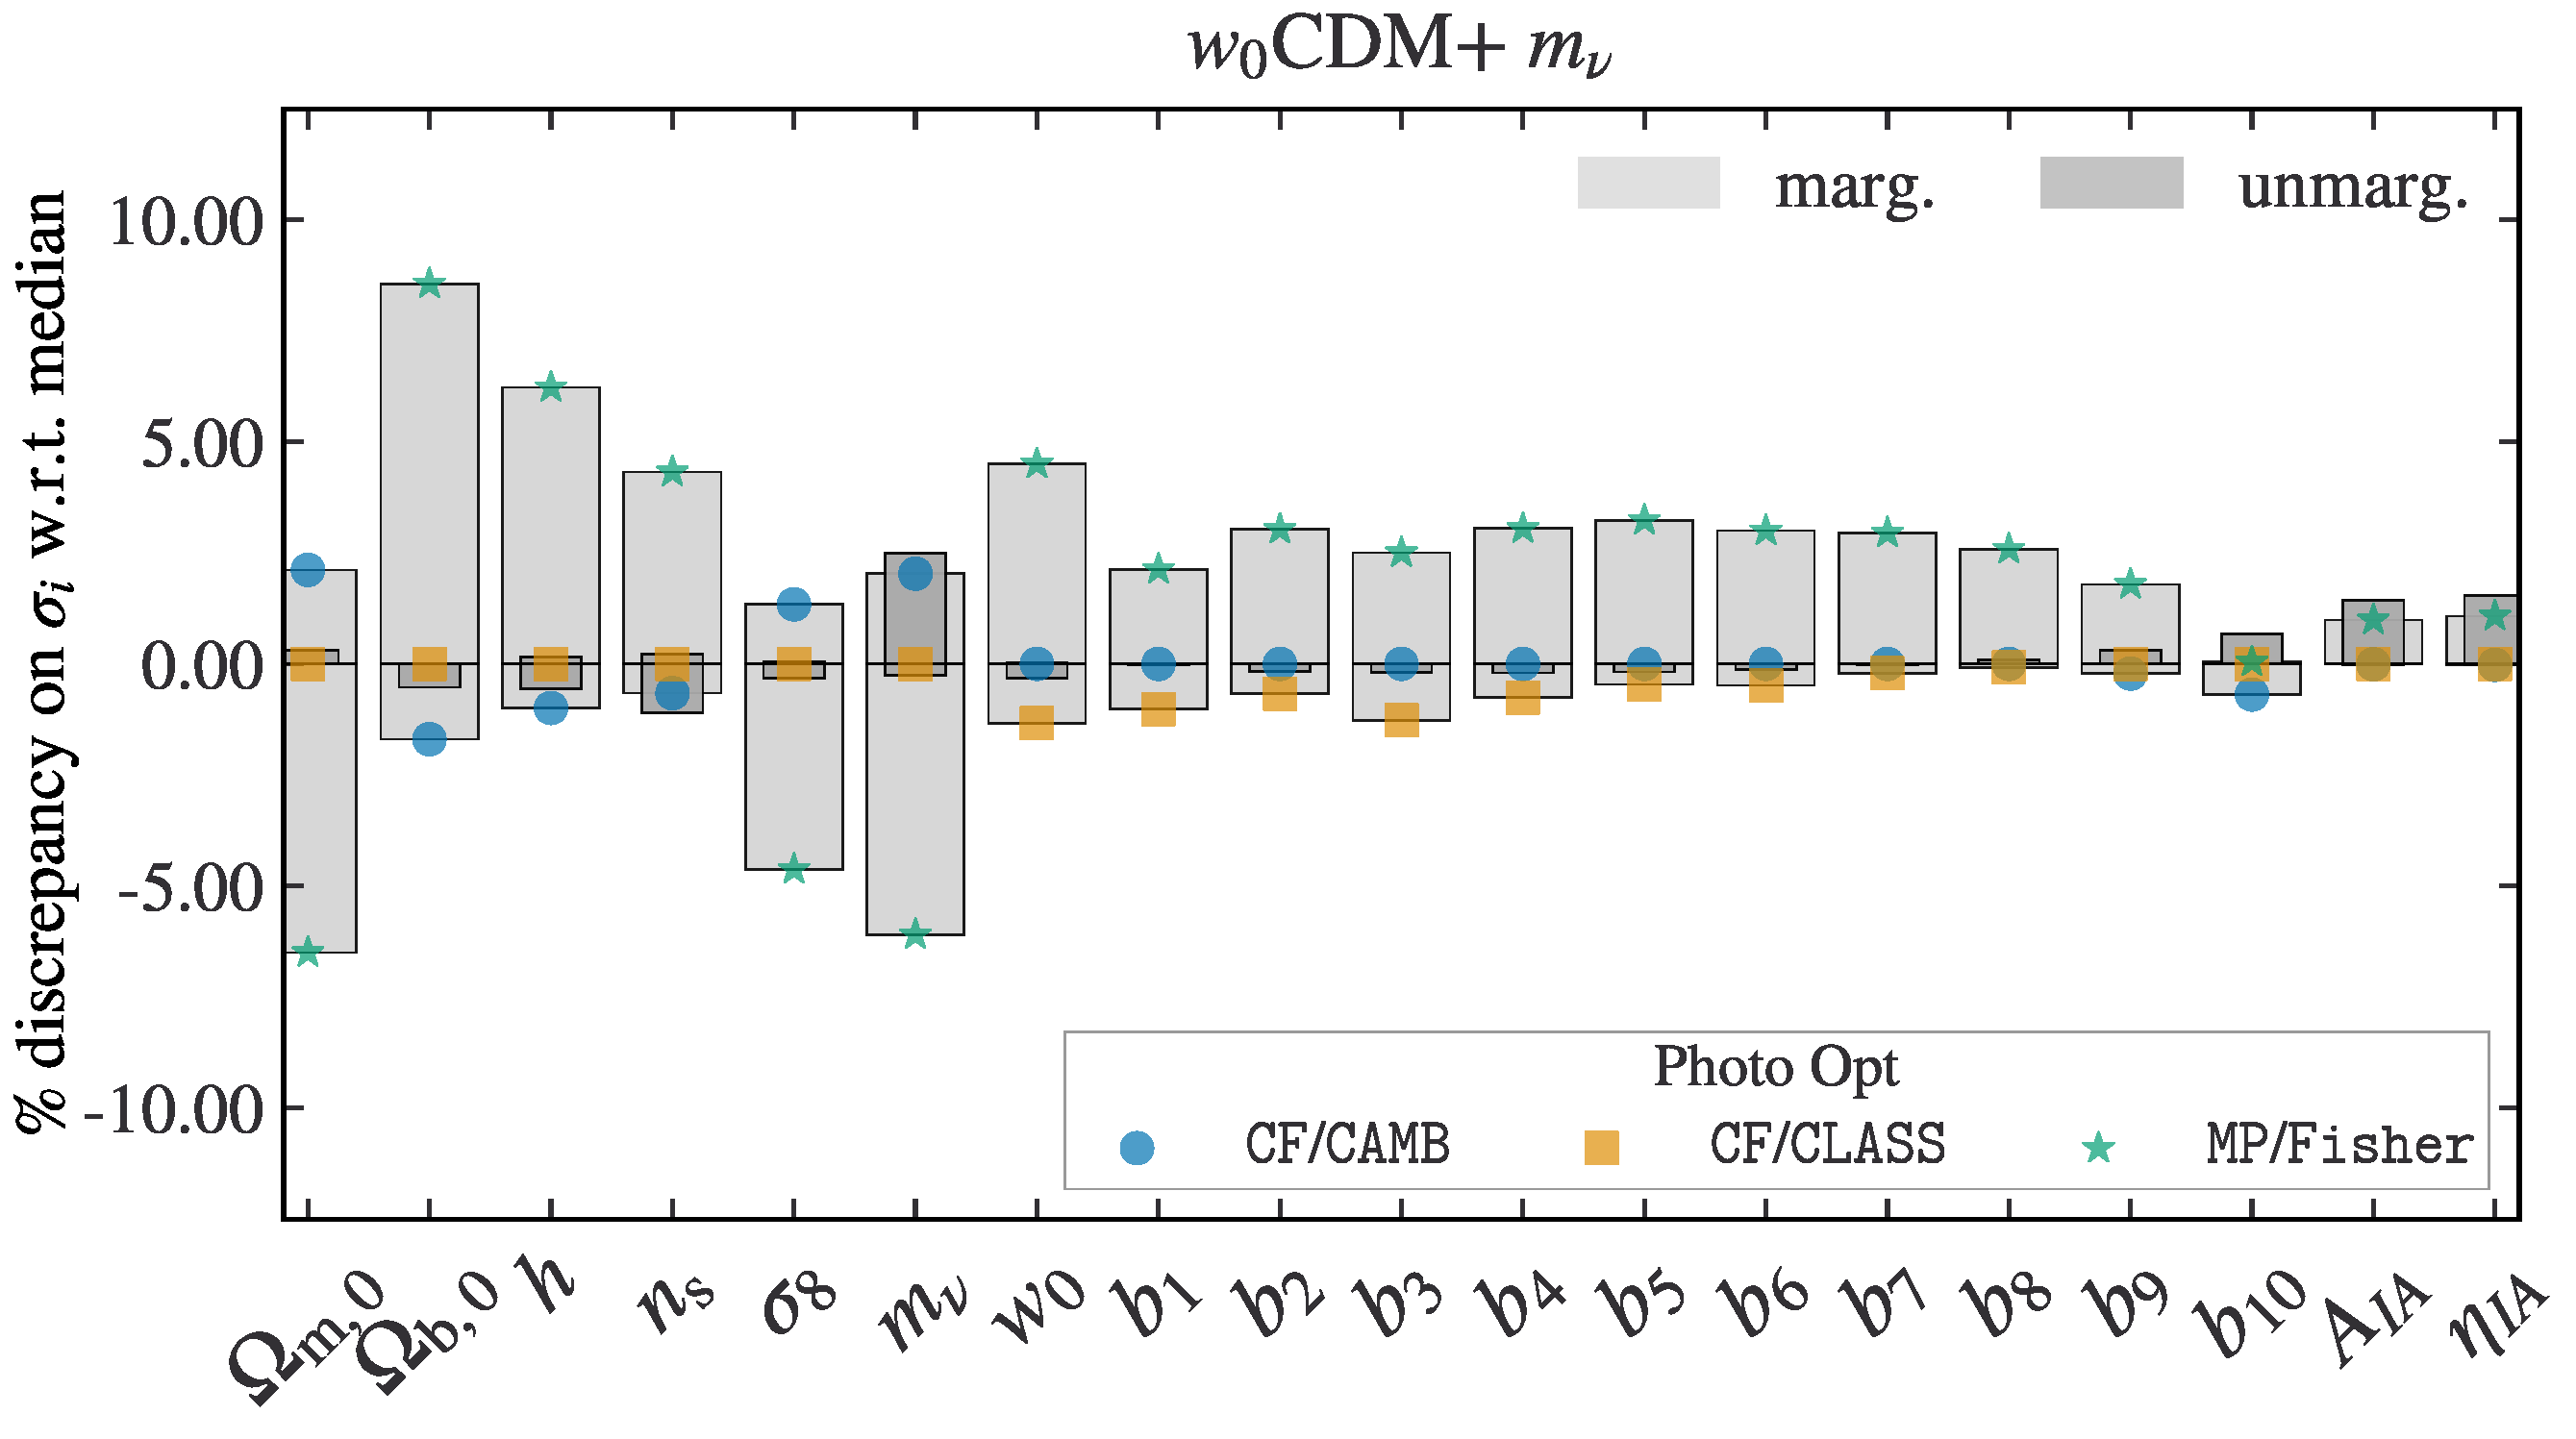
\includegraphics[width=\textwidth]{../plots/Photo_Opt_mnu+w0_error_comparison.pdf}
    \end{subfigure}
    \hfill
    \begin{subfigure}[b]{0.49\textwidth}
        \centering
        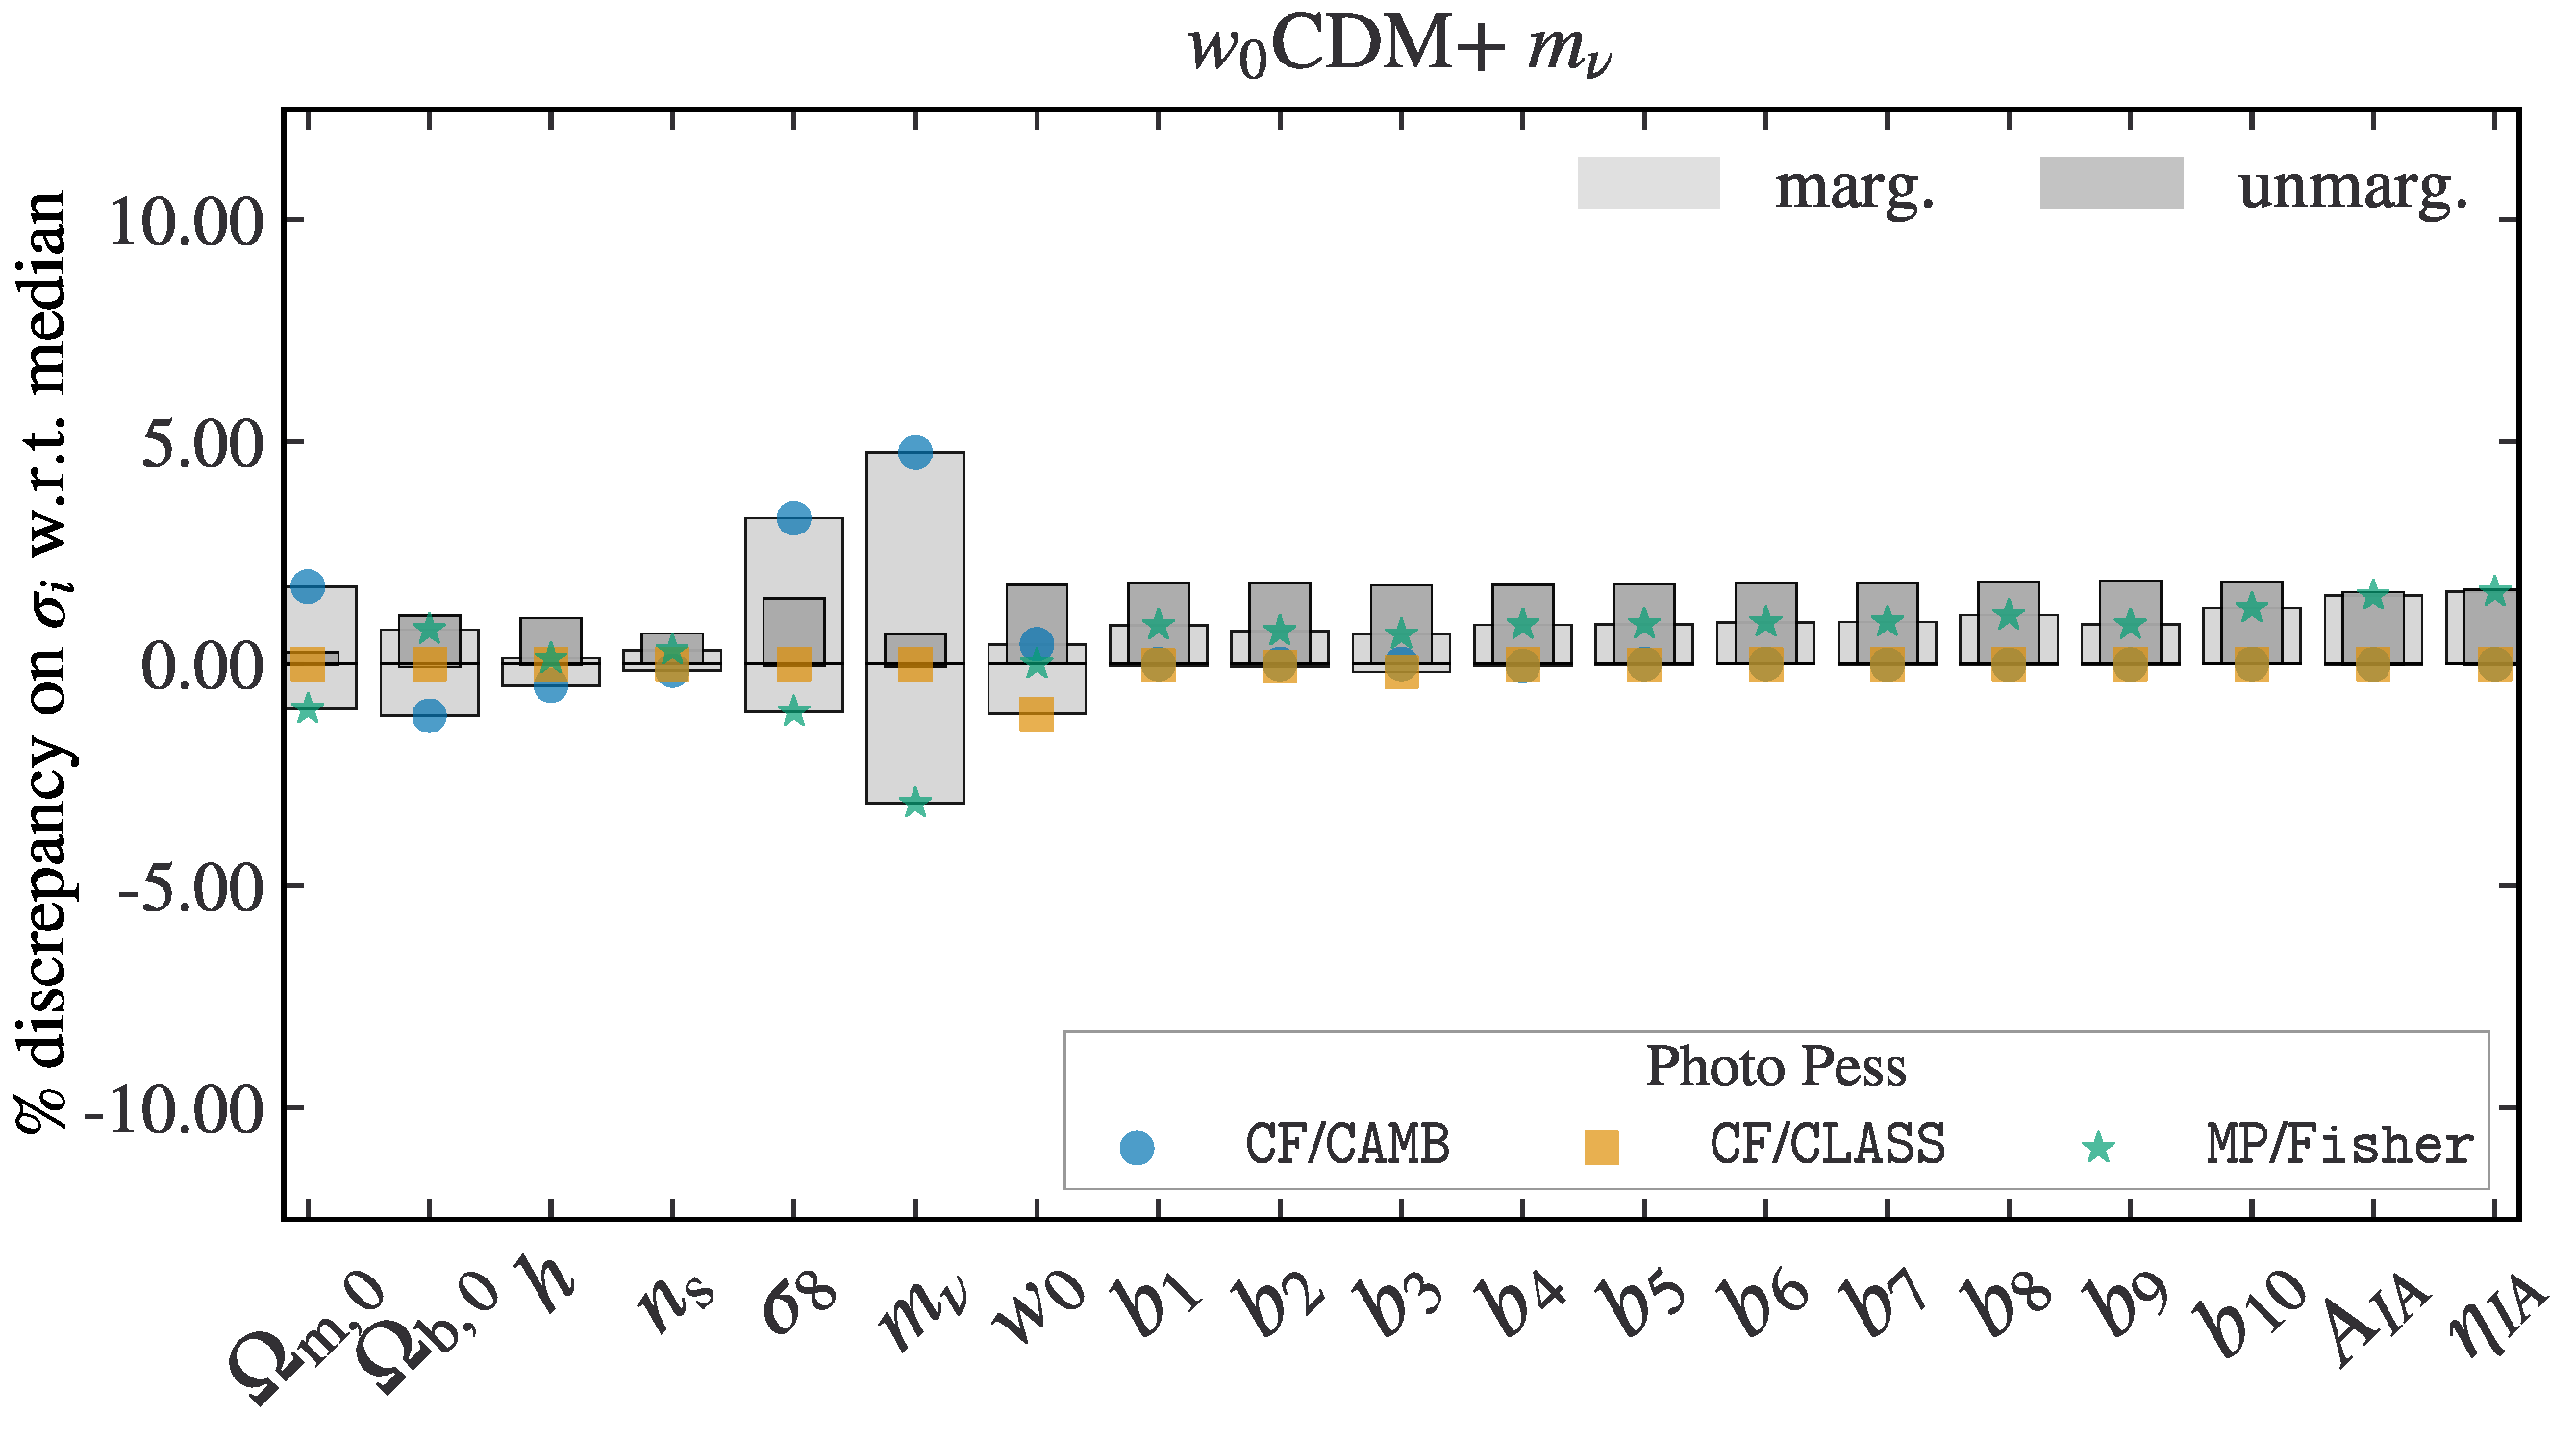
\includegraphics[width=\textwidth]{../plots/Photo_Pess_mnu+w0_error_comparison.pdf}
    \end{subfigure}    
       \label{fig:Comparison_w0M} 
\end{figure}
\begin{figure}
    \centering
    \caption{Same as figure \ref{fig:Comparison_w0wa} but for the $\Lambda$CDM+$m_\nu+\neff$ model}
    \begin{subfigure}[b]{0.49\textwidth}
        \centering
        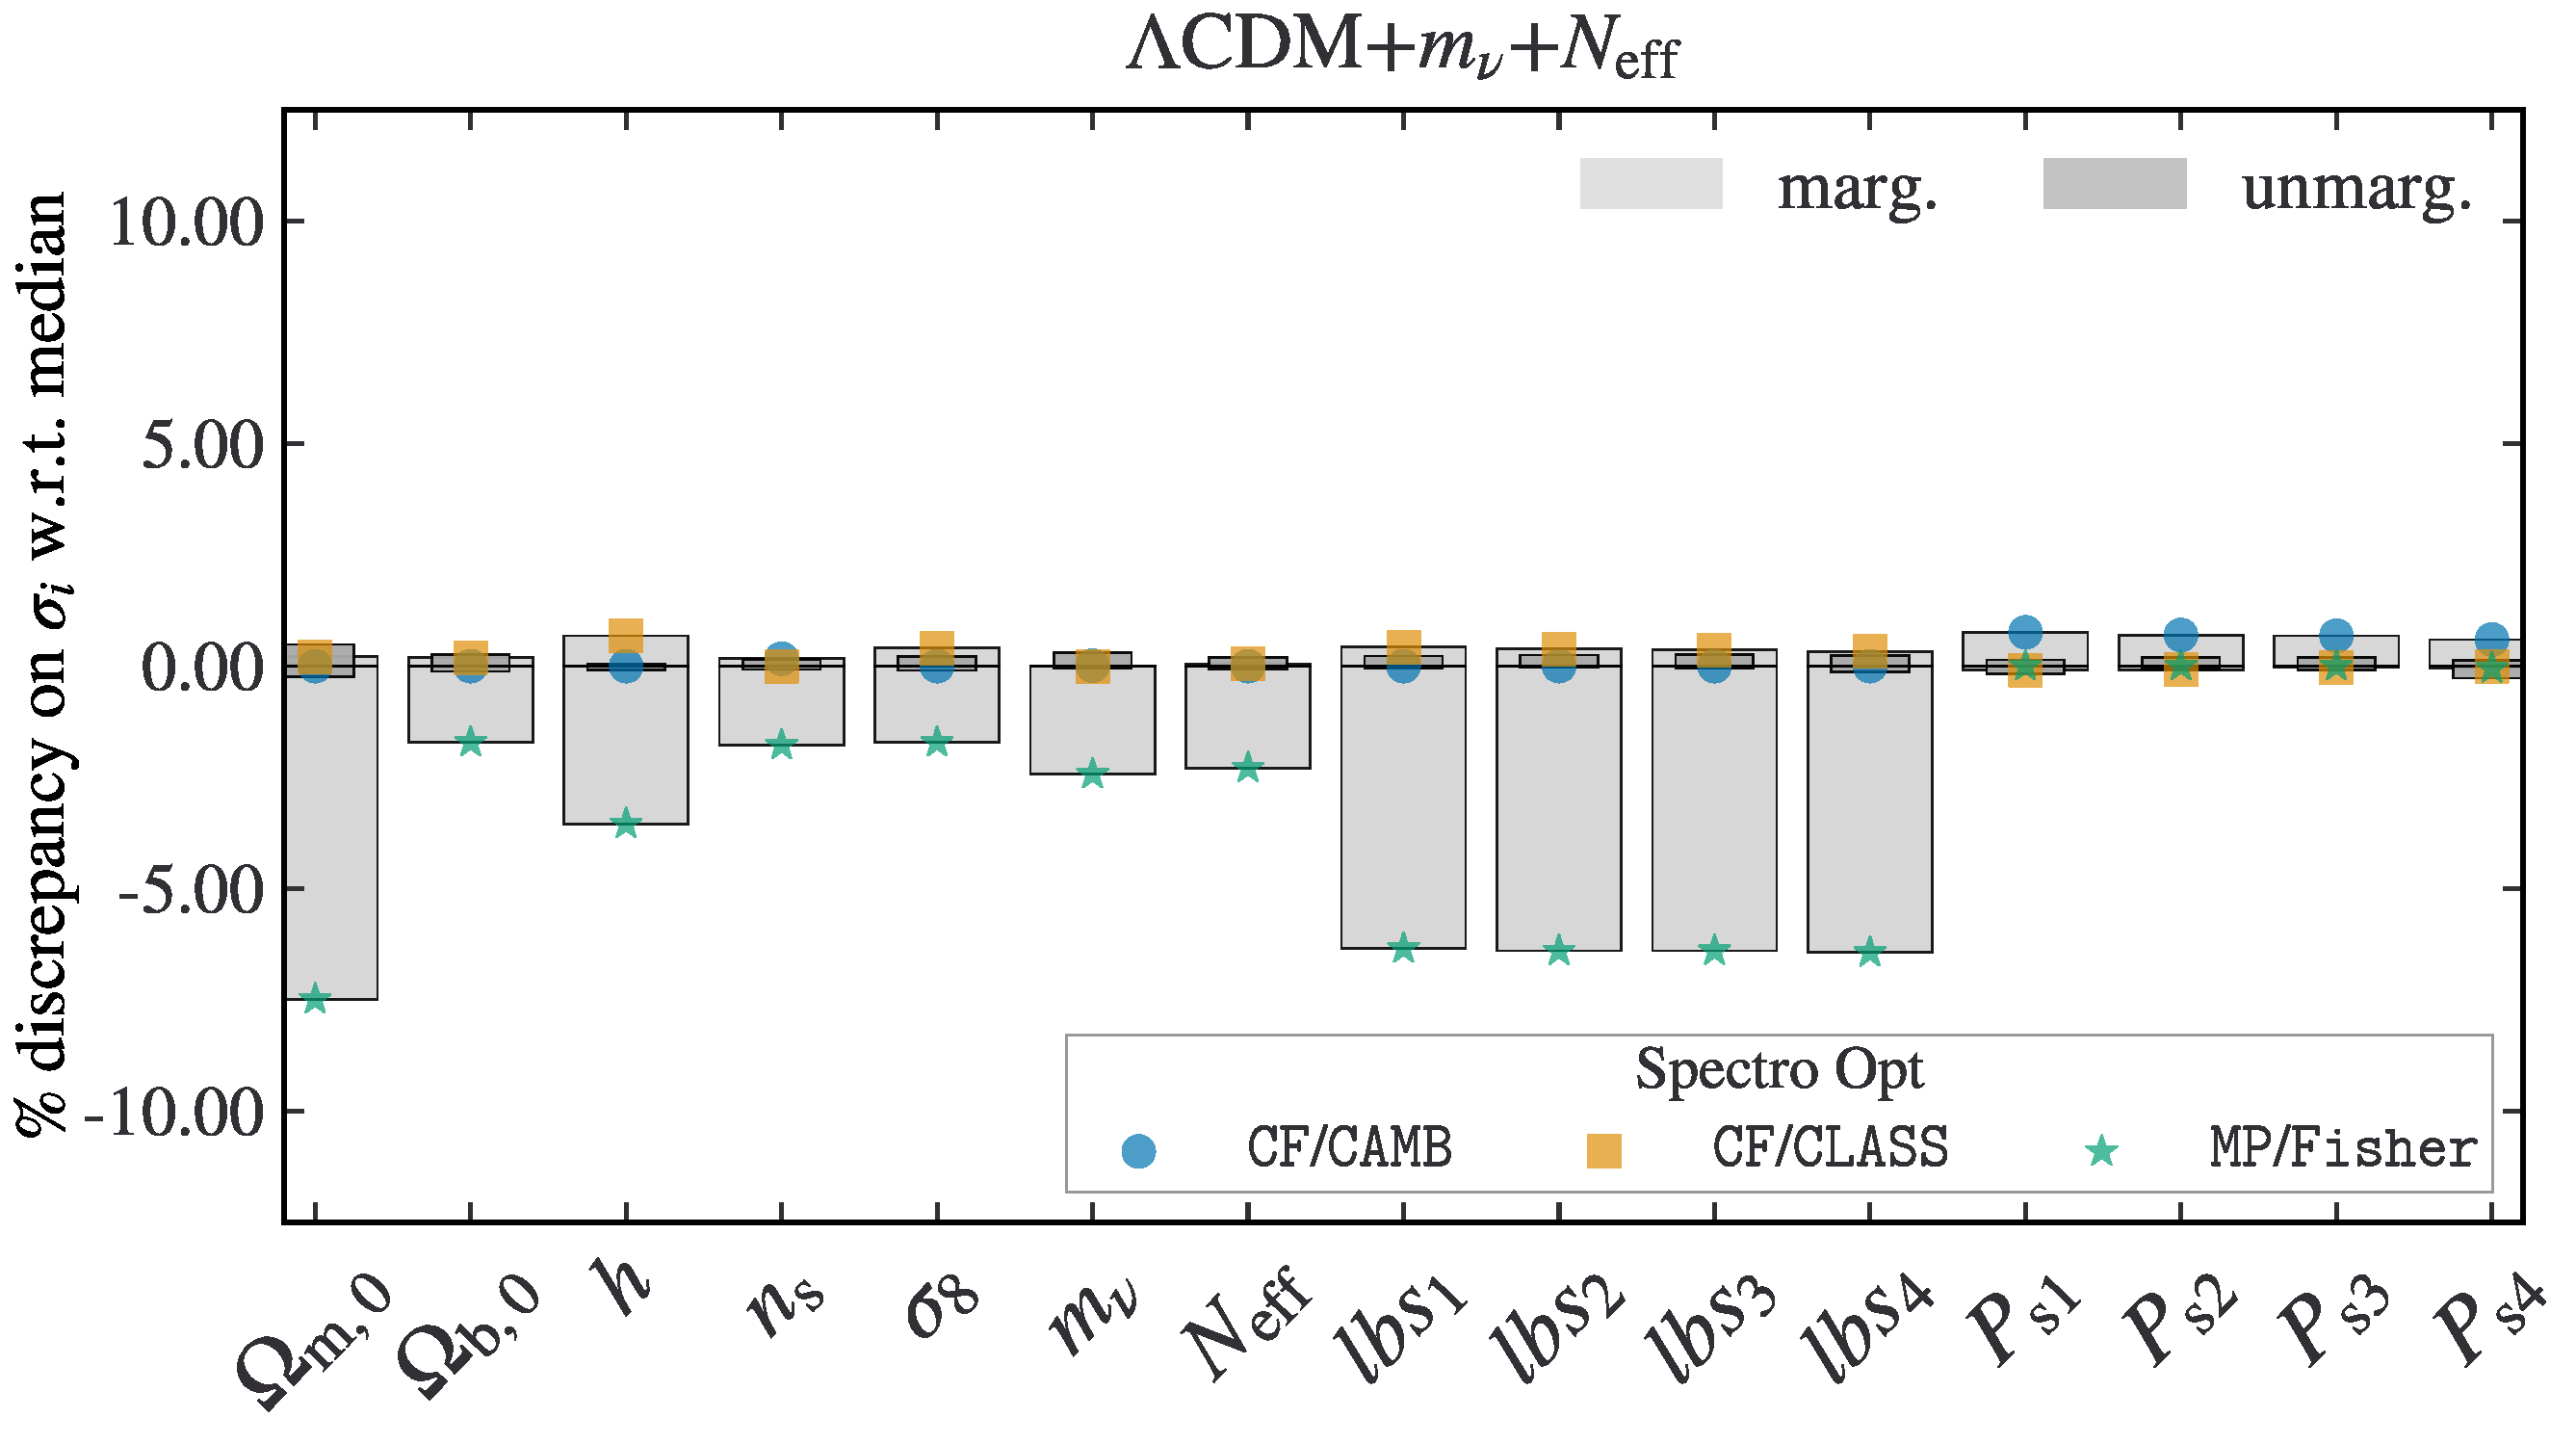
\includegraphics[width=\textwidth]{../plots/Spectro_Opt_mnu+Neff_error_comparison.pdf}
    \end{subfigure}
    \hfill
    \begin{subfigure}[b]{0.49\textwidth}
        \centering
        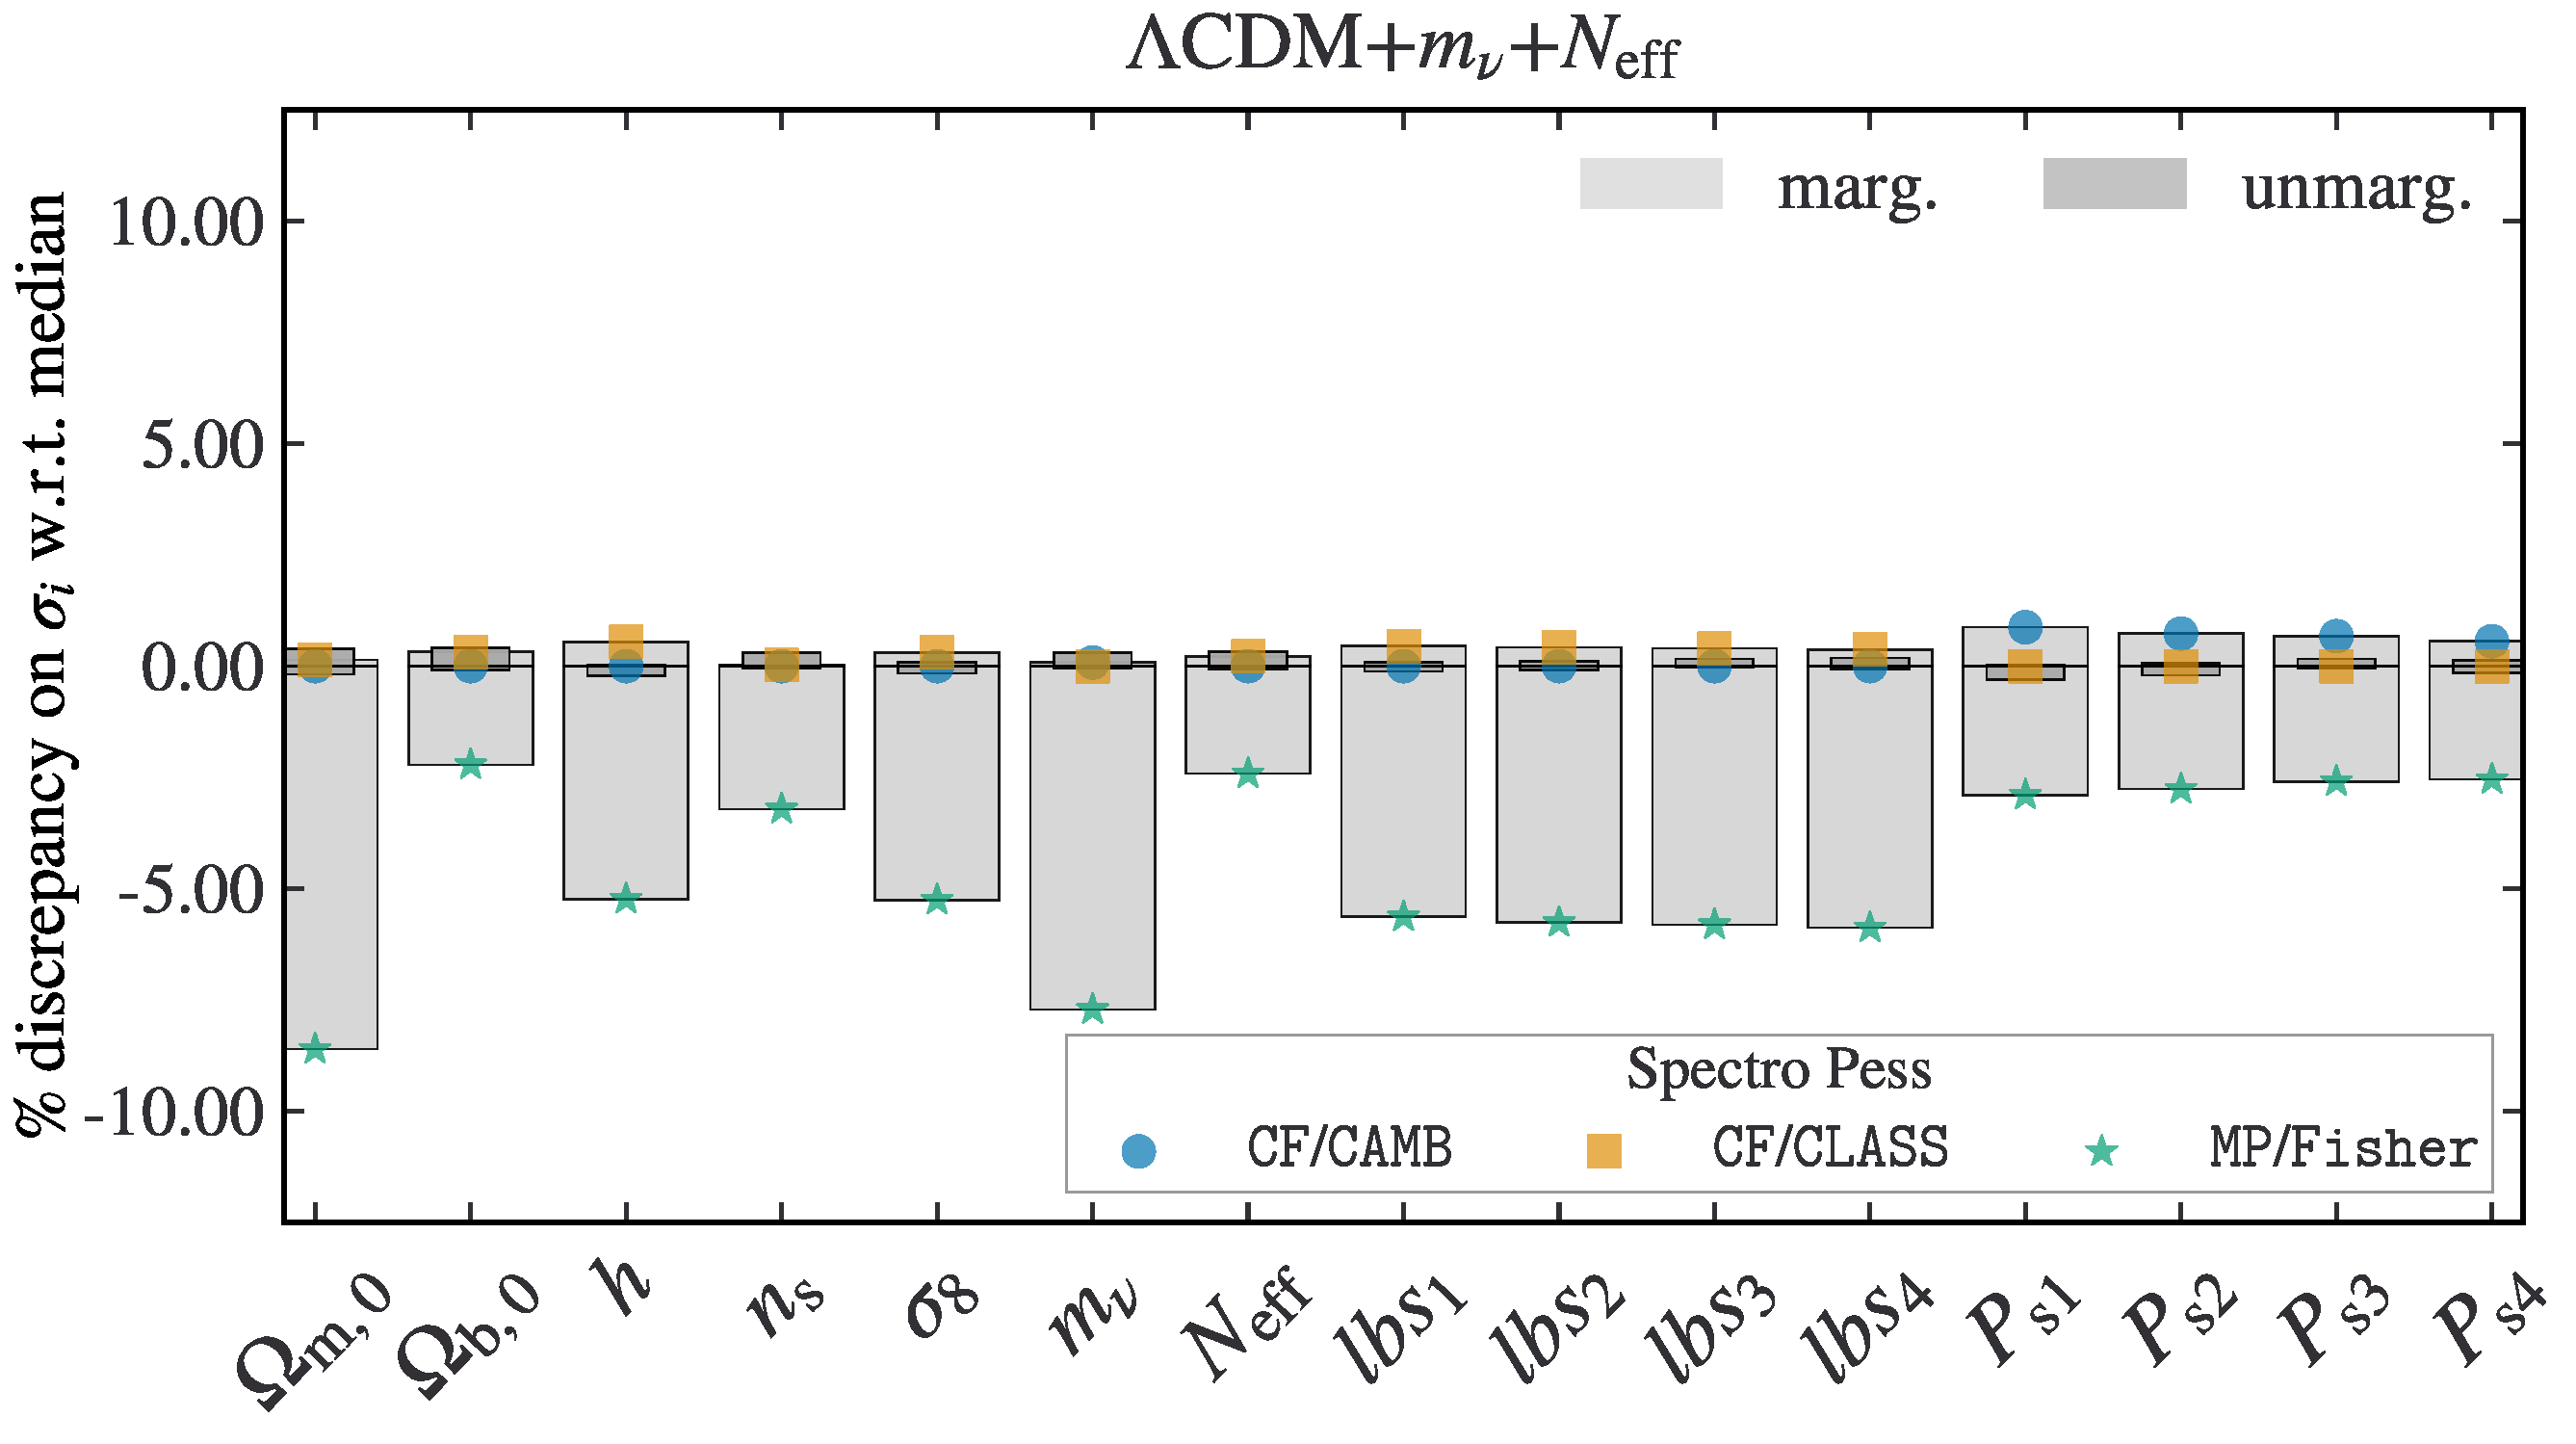
\includegraphics[width=\textwidth]{../plots/Spectro_Pess_mnu+Neff_error_comparison.pdf}
    \end{subfigure}\\
    \begin{subfigure}[b]{0.49\textwidth}
        \centering
        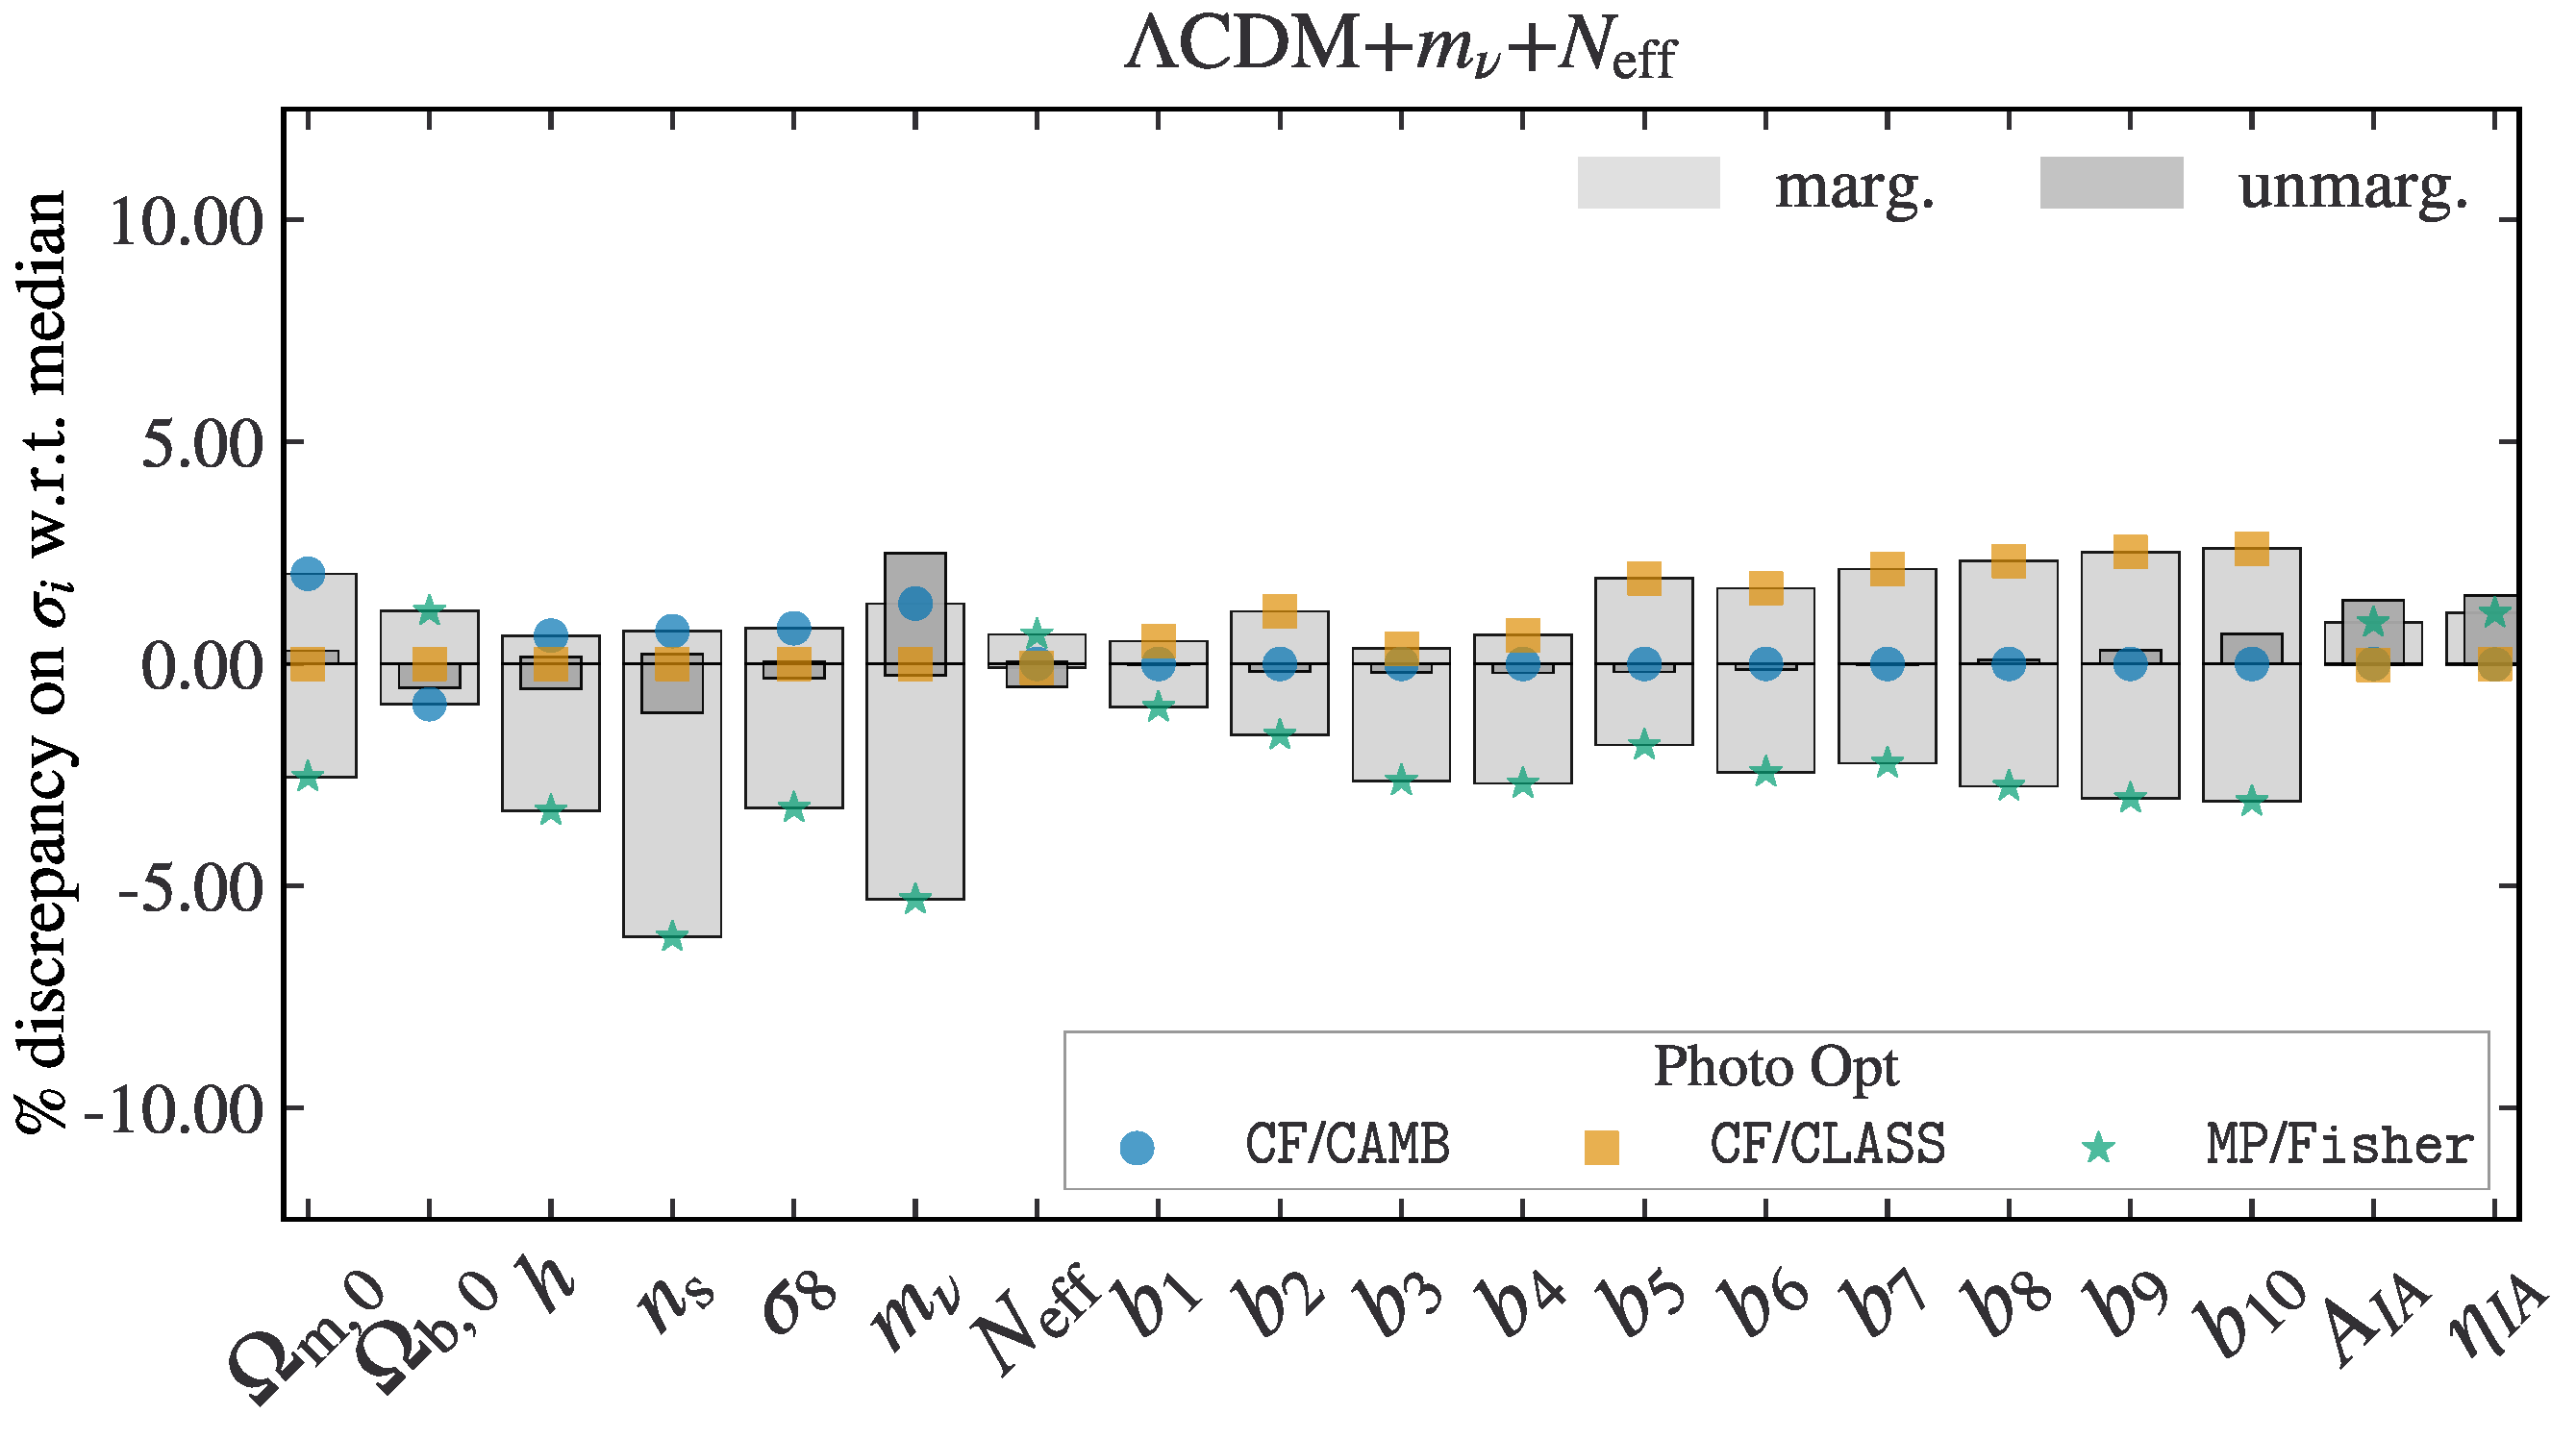
\includegraphics[width=\textwidth]{../plots/Photo_Opt_mnu+Neff_error_comparison.pdf}
    \end{subfigure}
    \hfill
    \begin{subfigure}[b]{0.49\textwidth}
        \centering
        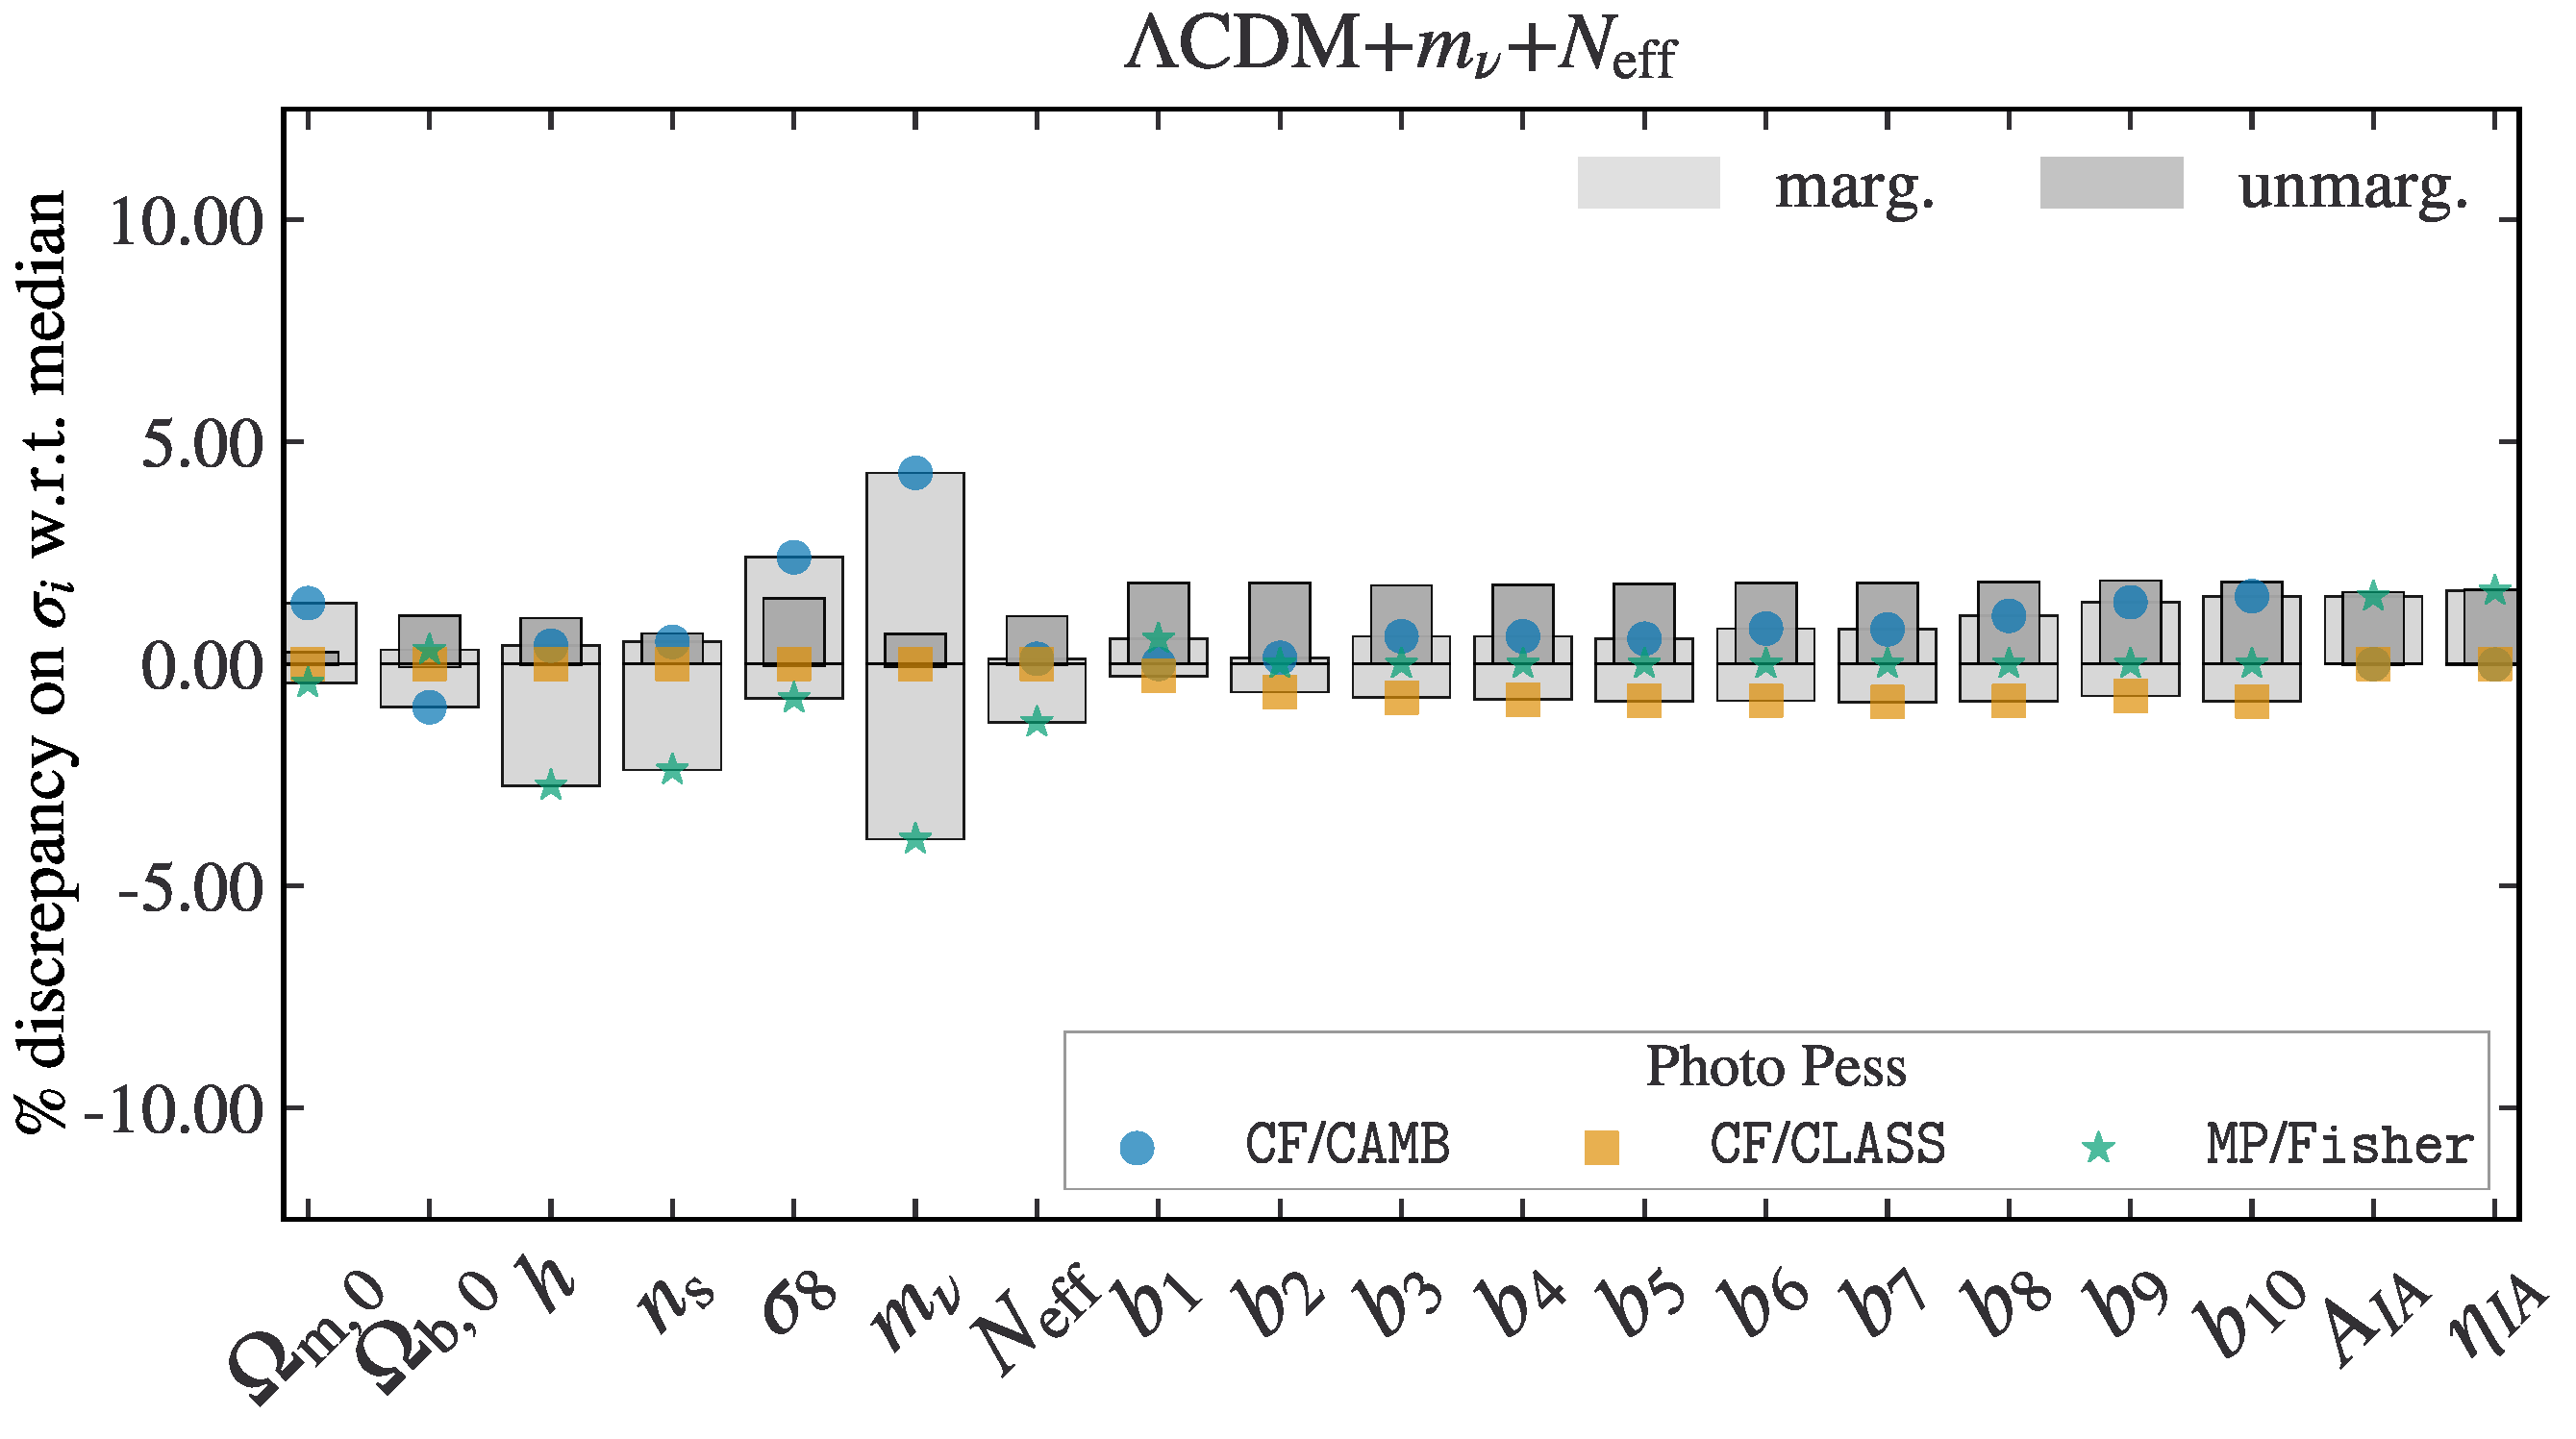
\includegraphics[width=\textwidth]{../plots/Photo_Pess_mnu+Neff_error_comparison.pdf}
    \end{subfigure}    
       \label{fig:Comparison_MN} 
\end{figure}
After careful setting of the input parameters and precision settings of our two EBS, the next step is to validate our forecasting results. For this, we will first discuss the choices we made in our forecasting pipeline. The first choice we have is for the derivate method. As we have discussed, in \cosmicfish the first-order derivate of the observable can either be calculated using an equal-sided three-point derivative (3PT), or a four-point forward derivative (4PT\_FWD). They both represent the two numerical derivatives that were introduced last chapter. For this test, we have compared the one-dimensional marginalized and unmarginalized errors obtained via \cosmicfish. We use \camb as the underlying EBS. We denote the \cosmicfish pipelines as either \cosmicfish:\camb or \cosmicfish:\class depending on the underlying EBS. The comparison is found in figure \ref{fig:comparison_derivs}. The derivative methods validate each other as the total deviation is within 5\% of each other for all parameters. We can see a systematic underprediction of the error when using the 4PT\_FWD derivatives instead of the 3PT derivatives. The agreement of the errors for the forecast is within 10\% of the mean for the case of varying all 9 cosmological parameters, thus the derivative is stable for all cosmological parameters. Due to the high precision of the 3 and 4-point derivates the difference in the unmarginalized errors is tiny hard to see on the plot. The error of those derivatives ar of the order of $h^2$ with $h$ already at 1\%. We can use two derivative methods for the rest of our forecast. We will use the 3PT derivatives in this work.\\
The next free choice we had in our forecasting was the stepsize for the approximate neutrino mass. As we have said before the relative stepsizes for the cosmological parameters were chosen to be 1\% of its fiducial value (or simply 1\% for $w_a$). We chose a higher stepsize of 10\% for the massive neutrino as the neutrino mass only affects the matter power spectrum slightly. Too small steps always come with the risk that the change of the matter power spectrum is dominated by numerical noise. To check if the derivative with a relative stepsize of 10\% is numerically stable we did the forecast with higher stepsizes of 30\% and 50\%. The result of the comparison can be found in figure \ref{fig:comparasion_mnu_stepsize}. We can see that the derivative with a stepsize of 10\% is very stable as the errors of the higher stepsize choices are within 5\% of each other. Since we have shown that the validation holds for the case with all 9 cosmological parameters, it is also valid for our validation cases with fewer parameters. As the error of a three-point numerical derivative is proportional to the stepsize squared, we will use a relative stepsize of 10\% for the approximate neutrino mass.\\
For each of the validation cases, we present the comparison for both survey settings and both probes. The comparasions are found in figures \ref{fig:Comparison_w0wa}-\ref{fig:Comparison_MN}. We show the errors of all cosmological parameters and nuisance parameters. We can see that all forecast errors are within 10\% of the median value and thus the validating is successful. With our careful setting of the precision parameters, we obtain very good agreement between the two Boltzmann codes. The biggest discrepancy between the different Cosmicfish FI methods is a 5\% difference in the neutrino mass. We believe this is due to residual small differences in the truncation of the Boltzmann hierarchy.\\
The comparison between \montepython and \cosmicfish is a bit worse with typical discrepancies of 5-10\%. The main contribution to this is that second-order derivatives are very sensitive to the choice of stepsize and there is no reasonable way to find the optimal one. The prescription for the stepsize was taken from \cite{casas2023euclid} where they optimized the FI element for $w_0-w_a$. This was chosen as that particular element was very sensitive to stepsizes due to the strong correlations. With this, we show that the prescription still works well enough for the validation but might be suboptimal when also varying the neutrino mass and the number of massless relics. Another reason for the worse agreement will be seen in the next section. It is the deviation from Gaussianity. This might be a subleading effect, as the deviation of the unmarginalized errors tends to be much smaller than marginalized ones. Typically, when there is non-guassianity, the double-sided second-order derivatives get an additional contribution which becomes visible in the unmarginalized errors.
\section{The validity of the Fisher approximation}
\begin{figure}
    \centering
    \caption{Comparison of the one and two-dimensional marginalized contours obtained by MontePython in MCMC mode ({\tt MP:MCMC}) with the contours of \cosmicfish:\camb and \montefisher. The contours depict the 68\% and 95\% confidence intervals for the $w_0w_a$CDM model respectively. We plot only the cosmological parameters for the different probes. On the left, we show the spectroscopic probe and on the right, we show the photometric probe.}
    \begin{subfigure}[b]{0.49\textwidth}
        \centering
        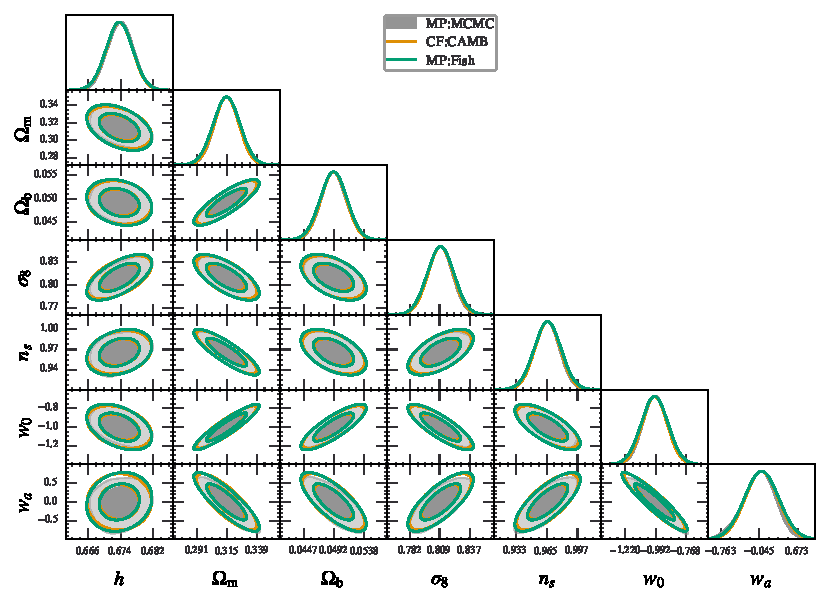
\includegraphics[width=\textwidth]{../plots/S_w0wa_validation.pdf}
    \end{subfigure}
    \hfill
    \begin{subfigure}[b]{0.49\textwidth}
        \centering
        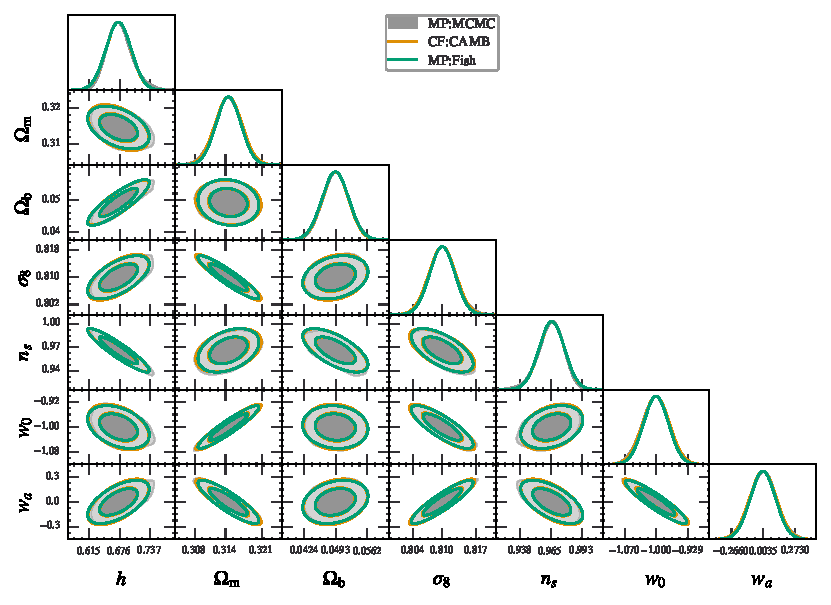
\includegraphics[width=\textwidth]{../plots/P_w0wa_validation.pdf}
    \end{subfigure}
       \label{fig:w0wa_triangle} 
\end{figure}
\begin{figure}
    \centering
    \caption{Same as figure \ref{fig:w0wa_triangle} but for the $w_0$CDM+$m_\nu$ model.}
    \begin{subfigure}[b]{0.49\textwidth}
        \centering
        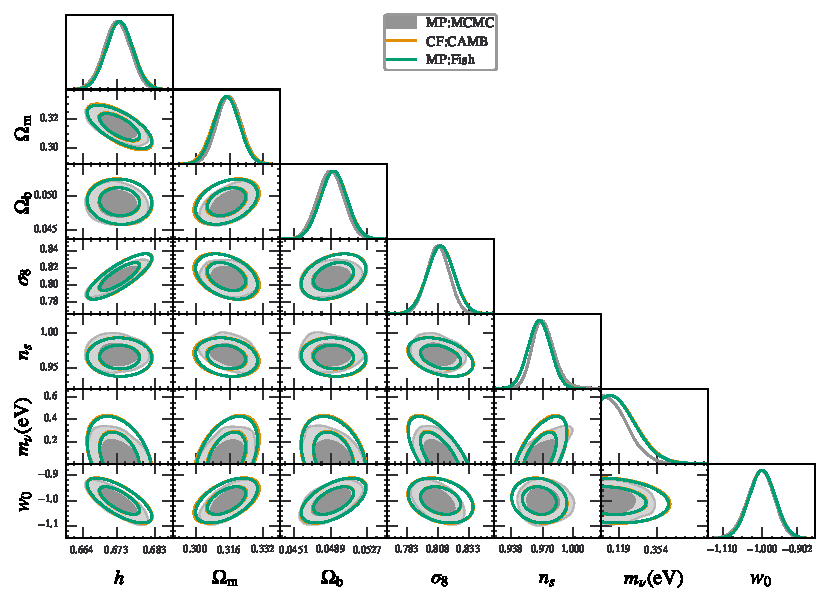
\includegraphics[width=\textwidth]{../plots/S_w0M_validation.pdf}
    \end{subfigure}
    \hfill
    \begin{subfigure}[b]{0.49\textwidth}
        \centering
        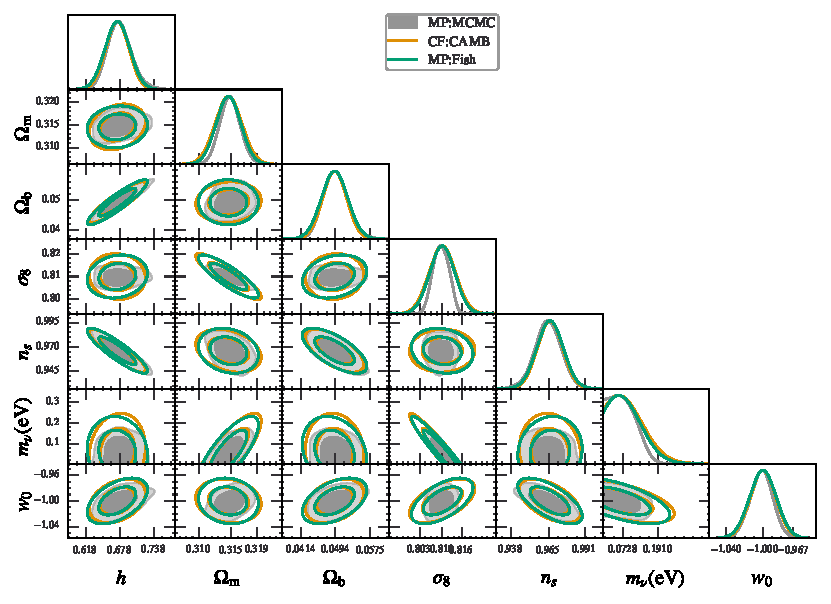
\includegraphics[width=\textwidth]{../plots/P_w0M_validation.pdf}
    \end{subfigure}
       \label{fig:w0M_triangle} 
\end{figure}
\begin{figure}
    \centering
    \caption{Same as figure \ref{fig:w0wa_triangle} but for the $\Lambda$CDM+$m_\nu+\neff$ model.}
    \begin{subfigure}[b]{0.49\textwidth}
        \centering
        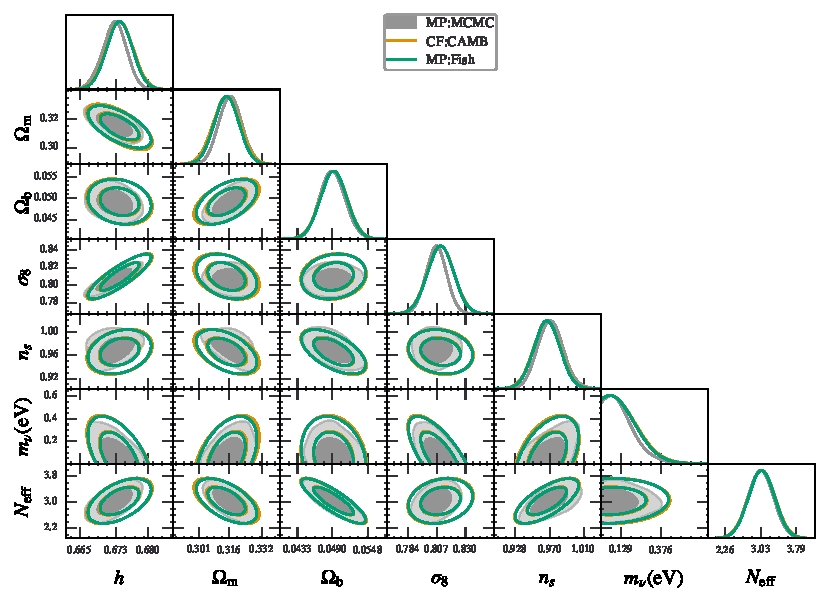
\includegraphics[width=\textwidth]{../plots/S_MN_validation.pdf}
    \end{subfigure}
    \hfill
    \begin{subfigure}[b]{0.49\textwidth}
        \centering
        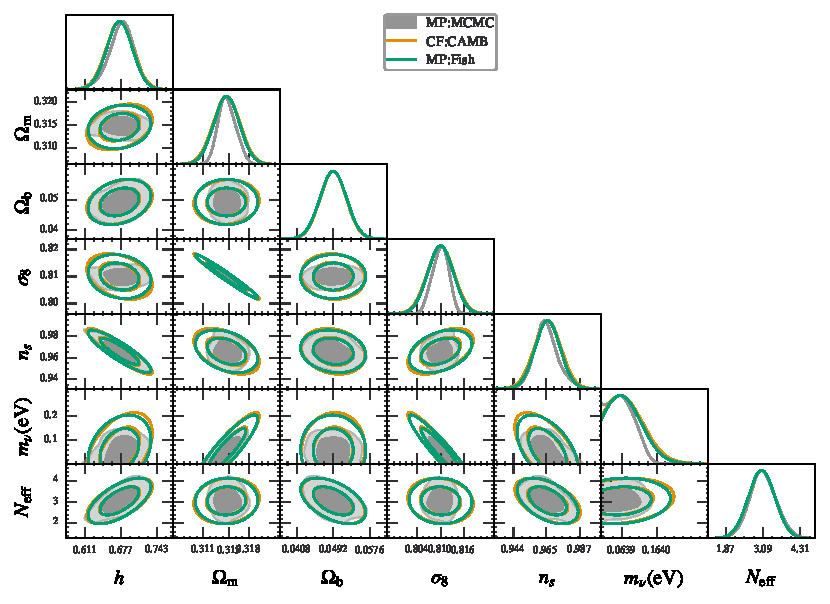
\includegraphics[width=\textwidth]{../plots/P_MN_validation.pdf}
    \end{subfigure}
       \label{fig:MN_triangle} 
\end{figure}
As we have stated before, the Validation of the FI results from \montefisher validates the same likelihood that we use for the MCMC. The next step is to check the validity of the FI method by comparison with the MCMC. We do the comparison only for the optimistic cases as the pessimistic cases have the same general tendencies. To compare the results we compare the one-dimensional marginalized posteriors and the two-dimensional contours. We obtain the MCMC results from \montepython running in Metropolis-Hastings mode and analyze them using GetDist. The comparison can be seen in figures \ref{fig:w0wa_triangle}-\ref{fig:MN_triangle}.\\
We can see in the contours of the $w_0w_a$CDM model that the MCMCs and the FI match very well. With this, we recover the validation from \cite{casas2023euclid} with our changes to the modelling and nonlinear corrections. This was expected as our modelling should only affect the contours of dark energy slightly due to the modelling of the nonlinear corrections. For the other parameters, the switch from \halofit to \hmcode came with the widening of the contours which is discussed further in the next section.\\
In the other two cases, we can see strong deviations in the MCMC from the FI approximation. Most striking in this are the posteriors of $m_\nu$.  The one-dimensional posteriors of $m_\nu$ show that the Fisher approximation holds well at the fiducial value, but starts to deviate in both directions. For lower values of $m_\nu$, the posteriors hits the theoretical prior, while for higher values it falls off more quickly than a Gaussian. We believe that the deviations of the other parameters can be explained solely by this.\\
In the spectroscopic probe of figure \ref{fig:w0M_triangle}, we can see clearly that the parameters that are uncorrelated with $m_\nu$ have next to no deviations from the Gaussian approximation while the stronger correlated parameters are affected more strongly. We see that due to the theoretical prior at zero mass important degeneracy directions get cut off and thus the posteriors deviate from the Gaussian approximation.\\
For higher values of the neutrino mass, we can also see a faster decay of the neutrino mass posterior. This is further amplified for the photometric probe. For that probe, the likelihood falls off so dramatically that the inside the 68\% confidence bound of the fisher coincides with the 95\% confidence bound of the MCMC. This has the effect that the strongly correlated parameters namely $\sigma_8$ and $\Omega_m$ not only get cut off at higher or lower values respectively, but also fall off quicker on the other side. We can also see a slight rotation of the FI contours for these parameters as the Gaussian approximation starts to fail even at the maximum likelihood.\\
We can see the same tendencies in the comparisons of figure \ref{fig:MN_triangle}. This further confirms our hypothesis that all deviations from Gaussianity are due to the prior and the deviation from a Gaussian normal distribution for the parameter $m_\nu$. With these results, we think that our implementations are fully validated, and also prove that to have a good forecast for neutrino parameters we have to move on from the standard FI formalism. 
\section{Bias from Modeling}
\begin{figure}
    \centering
    \caption{We show the effect of switching the formulation of our observables to use $P_{mm}$ instead of $P_{cb}$. We compare the results of the fisher forecast for the photometric optimistic using \cosmicfish:\class as our code.}
    \begin{subfigure}[b]{0.70\textwidth}
        \centering
        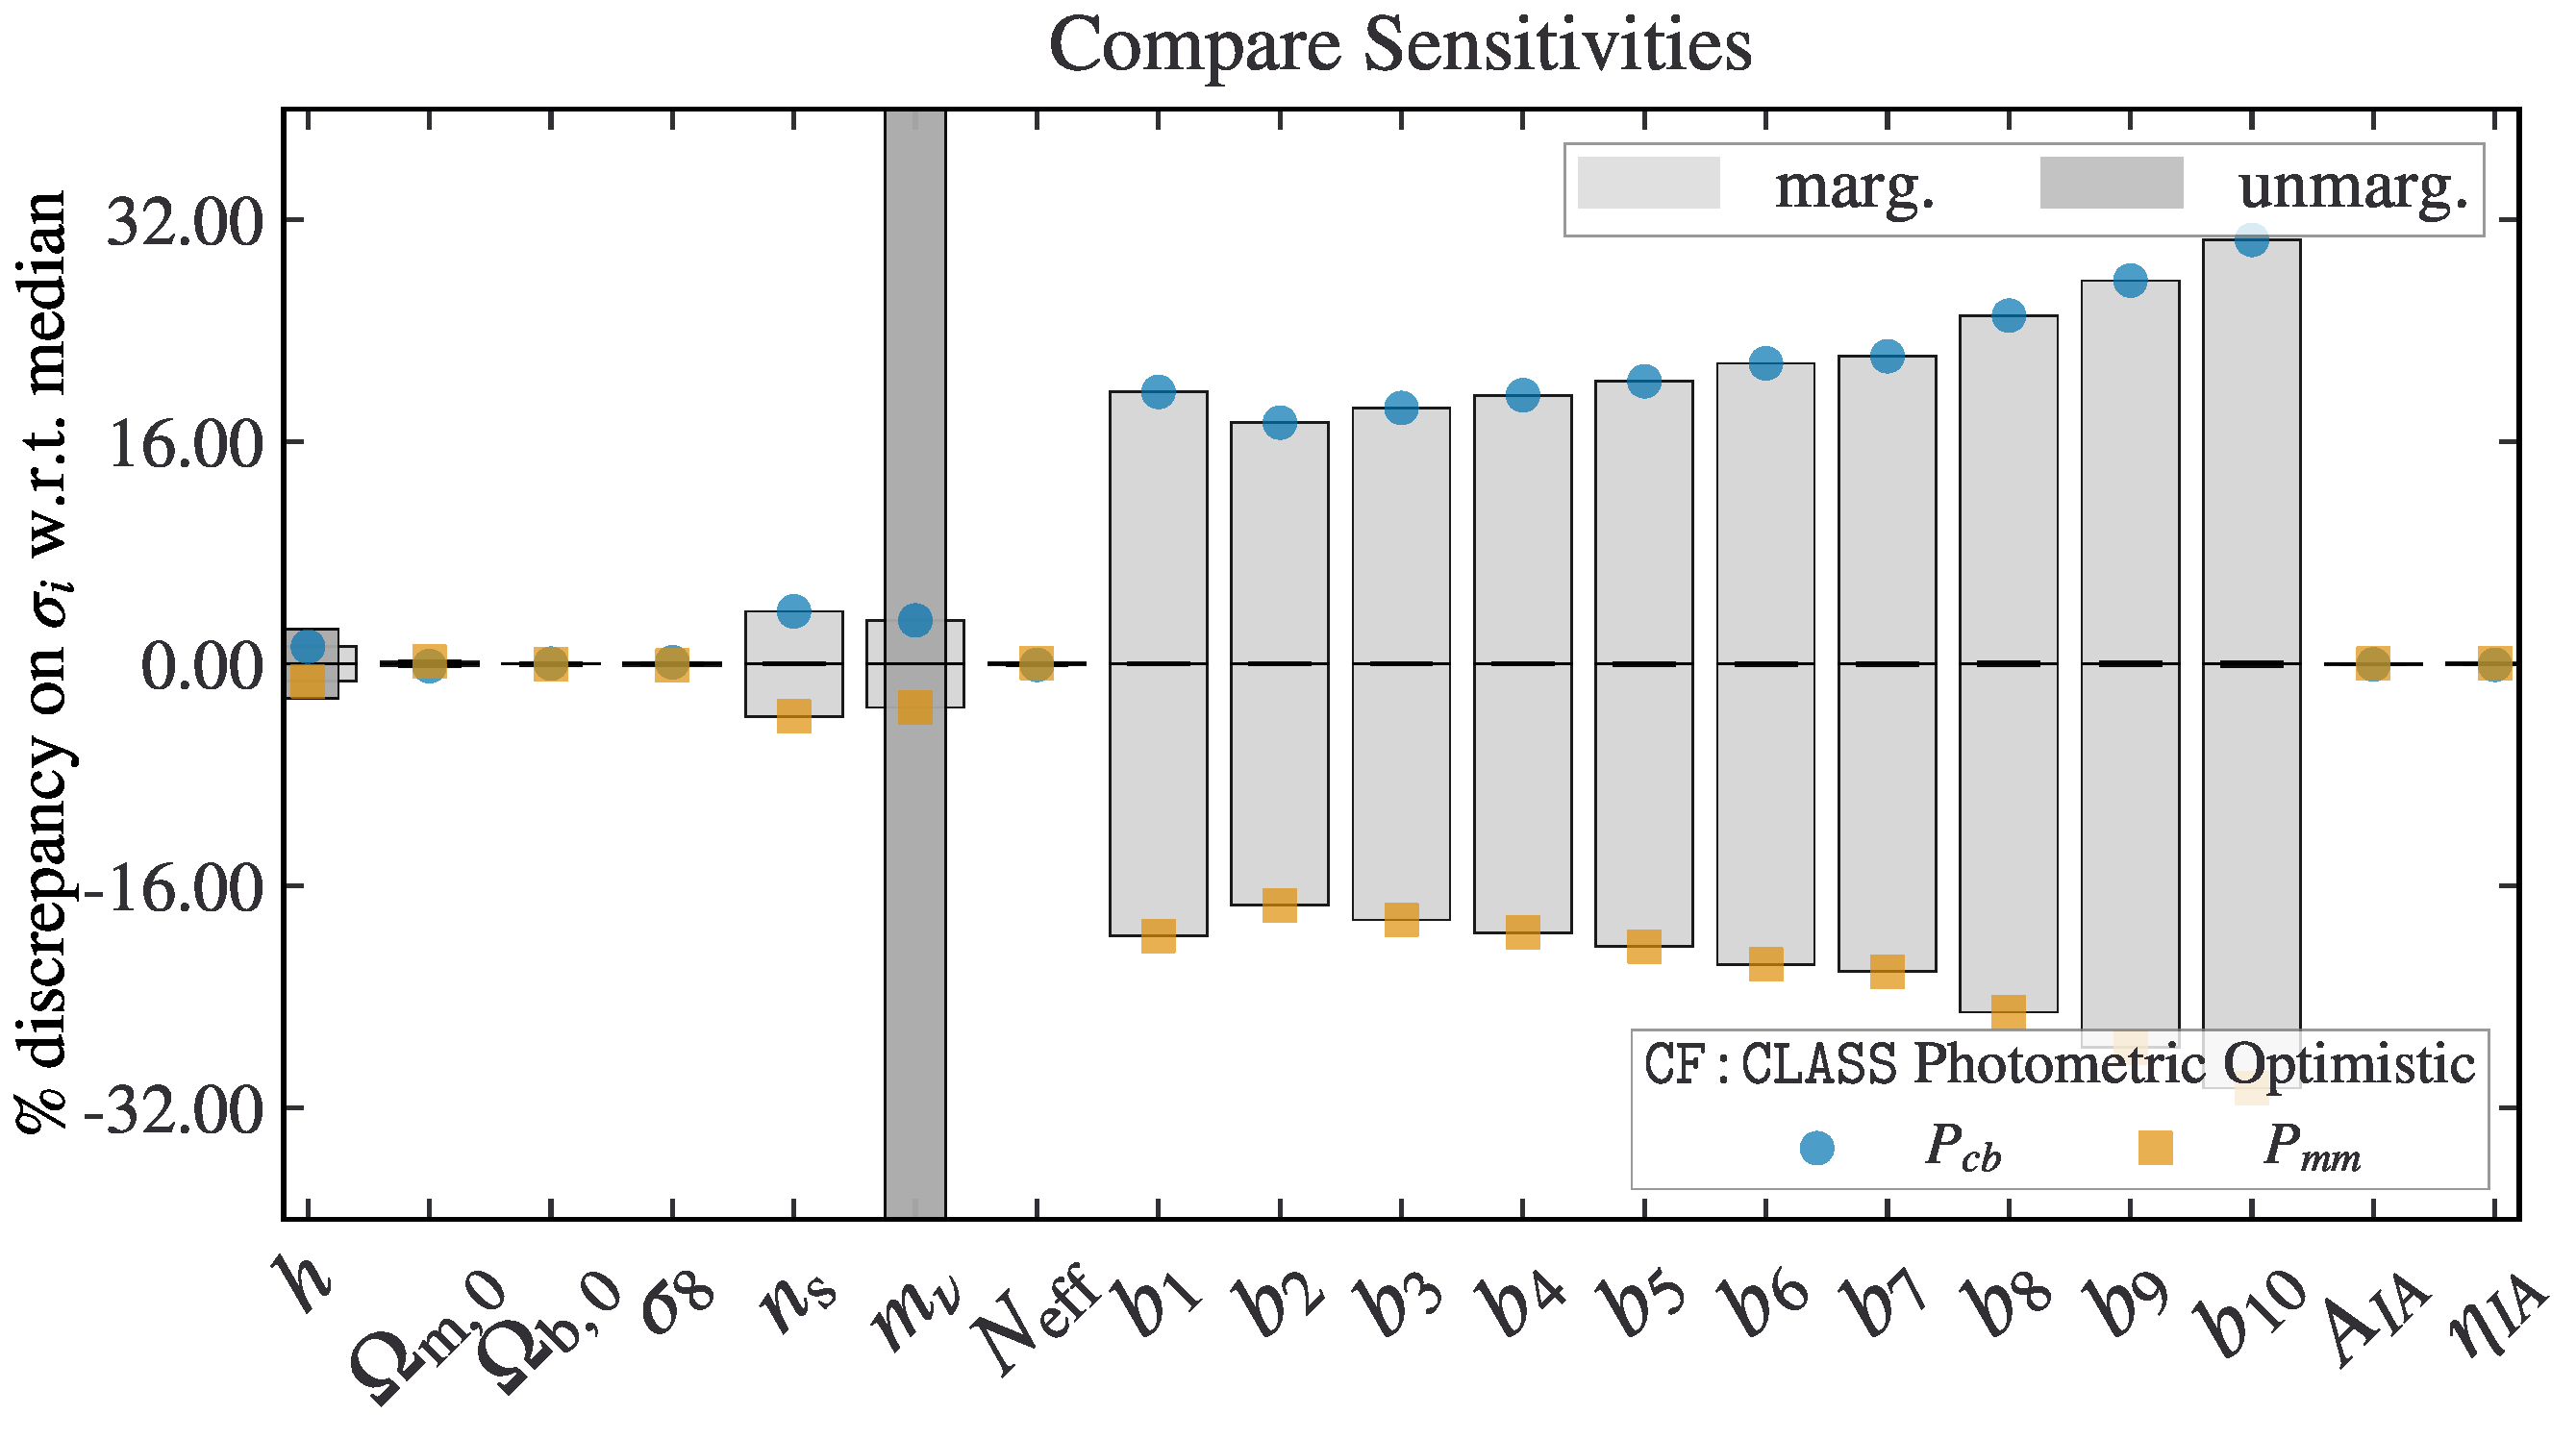
\includegraphics[width=\textwidth]{../plots/cosmopars_PmmvPcb_photo_Comparision_error_comparison.pdf}
        \caption{Comparision of the one-dimensional marginalized and unmarginalized errors obtained by either using $P_{mm}$ to formulate our observables or $P_{cb}$. For the parameter $m_\nu$ the difference in the unmarginalized error goes outside of the frame and is of the order of 43\% away from the mean.}
        \label{fig:dotsPcbVPmm}
    \end{subfigure}
    \\
    \begin{subfigure}[b]{0.70\textwidth}
        \centering
        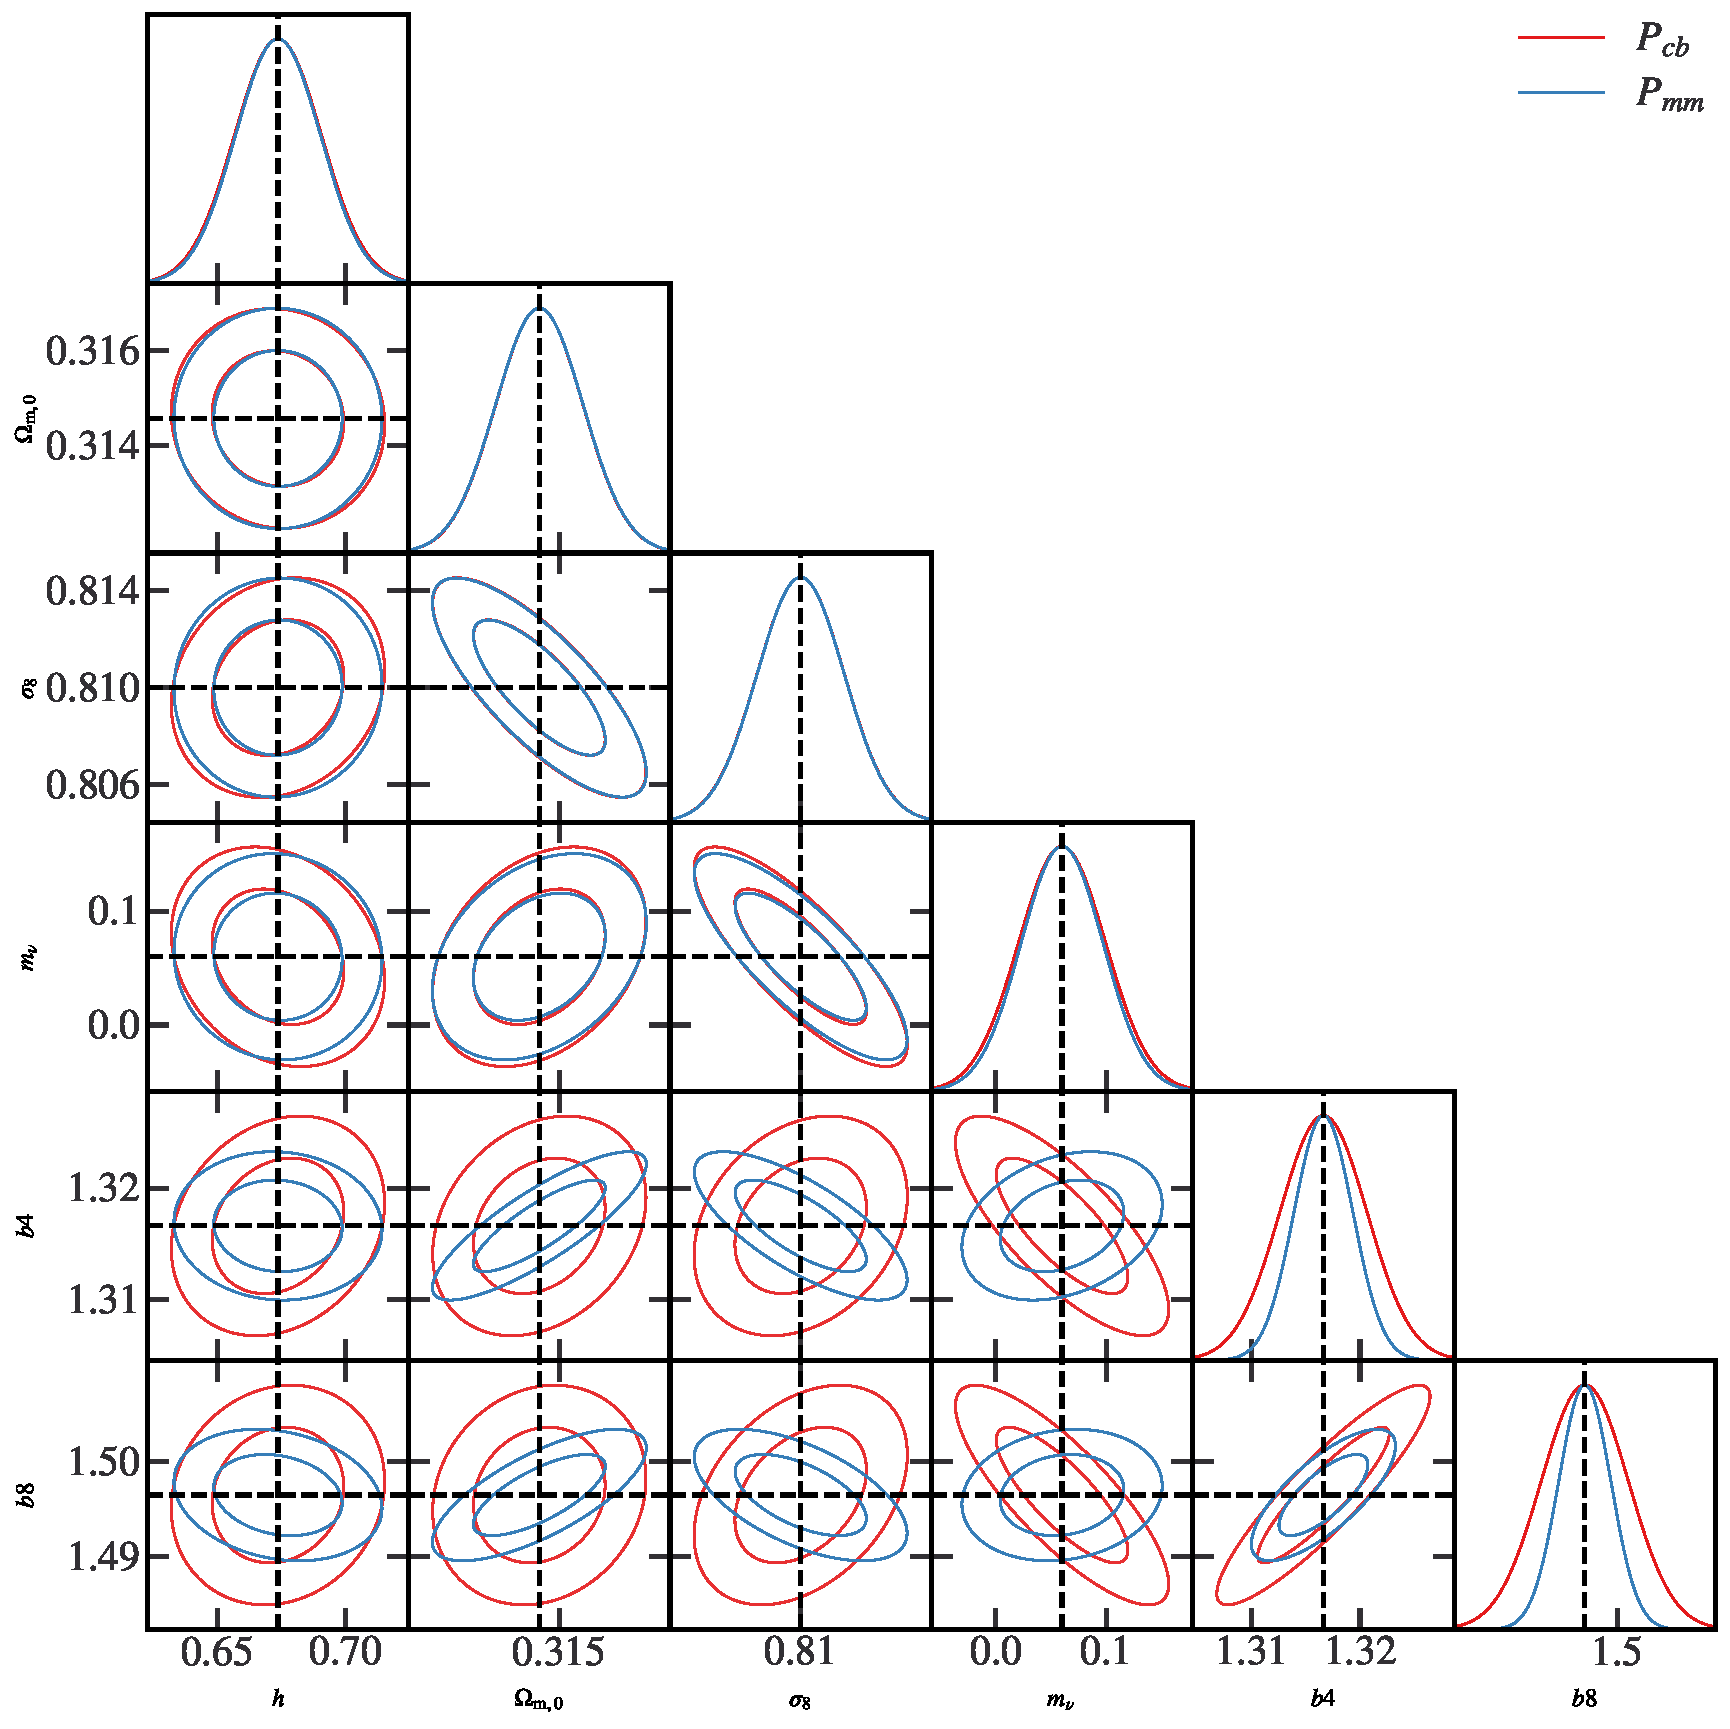
\includegraphics[width=\textwidth]{../plots/nonuicance_PmmvPcb_photo_Comparision_contours.pdf}
        \caption{Comparision of the one and two-dimensional marginalized FI contours for the two formulations. We marginalized over other cosmological and nuisance parameters as their trends are the same.}
        \label{fig:trianglePcbVPmm}
    \end{subfigure}
       \label{fig:PcbVPmm} 
\end{figure}
Before we come to the forecasting results, we wanted to have a brief discussion about the effects of our modelling. We first discuss our switch from the total matter power spectrum to the CDM+baryon power spectrum. As we have discussed before due to massive neutrinos the CDM+baryon matter power spectrum is suppressed by a factor $\sim(1-6f_\nu)$ on scales smaller than the minimum clustering scale $k_\mathrm{min}$. We have also discussed how this translates into a shift of the order $\sim(1-8f_\nu)$ for the total matter power spectrum. This means that overall the formulation of the likelihood is less sensitive to the neutrino mass when changing from $P_{mm}$ to $P_{cb}$. When doing a parameter inference it would have two effects. Firstly, due the to power spectra less depending to the neutrino mass, their constraints get wider. Secondly, if we assume that our description of the galaxy power spectrum would be the truth of the underlying data, then trying to fit the data with the 'wrong' description would bias our parameters.\\
To exemplify this claim we can think about the following gedankenexperiment. Let's say we have a galaxy clustering probe that is only sensitive to the smallest scales. Then the data power spectrum with an underlying neutrino mass $m_\nu$ would be suppressed by a factor $(1-6f_\nu)$. When we would fit the data our model power spectrum would try to different values of $m'_\nu$ until the power spectrum matches the data. The problem is that the suppression of the model power spectrum is given by $(1-8f'_\nu)$. Since the probe only measures the suppressed power spectrum the inference code will be able to find a matching $f'_\nu$ to perfectly fit the data. We will find \begin{equation}
    6\,f_\nu \overset{!}{=} 8\,f_\nu' \quad\Longrightarrow\quad m_\nu' = \frac{3}{4}\, m_\nu,
\end{equation}
as the neutrino fraction is directly proportional to the mass. This effect is lessened by the fact that the minimum clustering scale is also proportional to the root of the neutrino mass. This can be used to break the biasing but since the dependence is less strong this biasing effect is still there.\\
To test both of these effects we did two separate analyses. We first wanted to check how much the inferred errors change when changing the prescription to use $P_{mm}$ instead of $P_{cb}$. As a simplification, we presume that the fiducial value of the galaxy bias does not change between the two runs, i.e. $\hat{b}=b$. This can be done as the forecast error should not depend on the actual value of the biases. To do our comparison, we compare the results for the photometric probe in optimistic settings, and we chose the $\Lambda$CDM+$m_\nu+N_\mathrm{eff}$ model.\\  
The results of this comparison are found in figure \ref{fig:PcbVPmm}. In the upper figure \ref{fig:dotsPcbVPmm}, we can see that the change in the inferred error for the cosmological parameters apart from the neutrino mass is negligible. This was expected as the effect of those parameters on the matter power spectrum and the CDM+baryon power spectrum is very similar. For the neutrino mass, we find a strong discrepancy of 80\% in the unmarginalized error while the marginalized error is more comparable. We also see a strong 40\%-80\% shift in the errors of the galaxy biases. We believe that these two effects are related to one another. Viz., the difference between the matter power spectrum and the CDM+baryon power spectrum can be absorbed by the biases. This is due to the definition of the galaxy bias. If we remember how it was defined we can see that on scales much smaller than $k_\mathrm{min}$
\begin{align}
    &&P_{gg}(k,z) = b^2(k,z)\,P_{mm}(k,z) &= \hat{b}^2(z)\,P_{cb}(k,z)\nonumber\\
    \overset{\approx}{\Longleftrightarrow}&& b^2(k,z)\,(1-f_\nu)^2\,P_{cb}(k,z) &= \hat{b}^2(z)\,P_{cb}(k,z).\nonumber
\end{align}
This means that the strength of the suppression of the matter power spectrum can be absorbed by accordingly shifting all galaxy biases enough to mimic the missing suppression. Furthermore, this leads to a change in the degeneracy directions of the biases concerning the other cosmological parameters. This effect of compensation can be seen in figure \ref{fig:trianglePcbVPmm}\\
For our next check, we wanted to perform a naive biasing test, where we generate our data vector using our more correct description using $P_{cb}$ and then fit it using the $P_{mm}$ description. The results of this test are found in figure \ref{fig:trianglePcbVPmm_biased} where we have picked out some indicative parameters. We can see how the posteriors of $m_\nu$ shift to lower values and hit the theoretical prior. This is due to the discrepancy between the suppression of the two power spectra. This effect is partially broken by adding the shearing probe. The angular power spectrum of weak lensing is calculated by the total matter power spectrum alone and thus independent of our modelling of the galaxy bias. The remaining shift of the neutrino mass induces a slight shift in $\Omega_m$ and $\sigma_8$ in their respective correlation directions. As we discussed, we can see how the bias parameters try to compensate for the reduction of $P_{mm}$ on the smallest scales by shifting to higher values. Their correlation with the cosmological parameters $\Omega_m$, $\sigma_8$ and $m_\nu$ shift again since they will need to compensate for additional shifts of the power spectra. This degeneracy is broken by the fact that the probes are also sensitive to intermediate ranges where the neutrino-induced suppression has not flattened out yet. To take care of this effect, we would have needed to switch to a scale-dependent galaxy bias in the $P_{mm}$ case.\newline
\begin{figure}
    \centering
    \caption{The biasing in the parameter inference when switching the prescription of the observables but fixing the data to $P_{cb}$. This is using the photometric probe in optimistic settings in a $\Lambda$CDM+$m_\nu+N_\mathrm{eff}$ model. In yellow, we show the posteriors if we try to fit the data using our $P_{cb}$ formulation. In grey, we show how we fit the data using our $P_{mm}$ formulation.}
    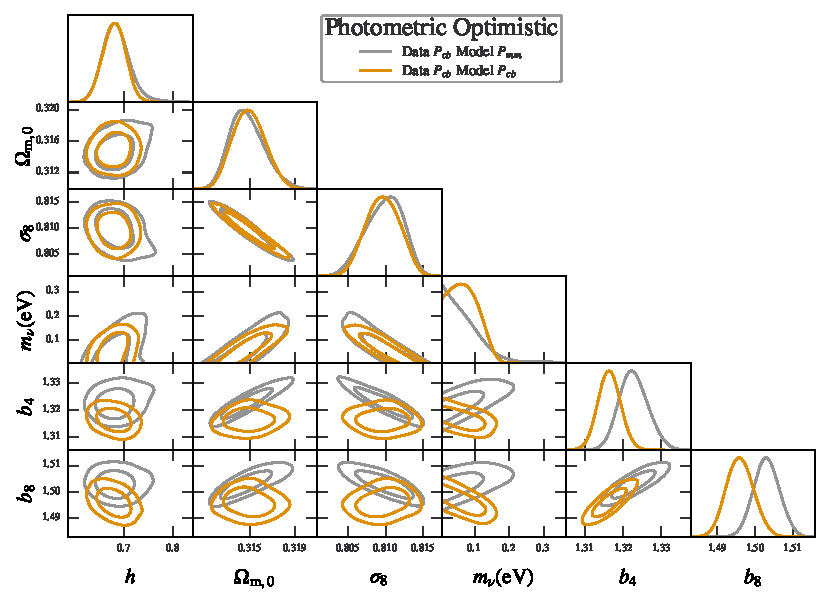
\includegraphics[width=0.9\textwidth]{../plots/P_MN_Pcb_v_Pmm_bias.pdf}
    \label{fig:trianglePcbVPmm_biased}
\end{figure}
\noindent Our next discussion will be about the switch from \halofit to \hmcode. As we had stated earlier, the difference between them is that \hmcode is a semi-analytical model and \halofit is a direct fit. This means they react slightly differently to a change in cosmological parameters. We will analyze this change in our first test as before.\\
All codes trying to predict the nonlinear power spectrum give slightly different results. It is unclear which of them describes the reality better. We know that \hmcode matches better simulations with massive neutrinos like the \Euclid flagship simulations so we use it for our forecast. To check how much this can bias, our results for our second test we fit different data with the same model. This essentially answers the question of how inferred parameters would shift if our nonlinear prescription did not match reality.\\
The results of the first test are found in the figure \ref{fig:triangle_HCvHM_biased}. We can see large discrepancies between the forecast errors for all parameters. The largest discrepancy is in the unmarginalized errors for the neutrino mass. There we have a  15\% discrepancy between the two codes. We believe this is due to the many different places where the \hmcode algorithm treats massive neutrinos, that do not get caught in the \halofit fitting formula. In the \halofit model the effect of massive neutrinos enters the total matter power spectrum while many effects of nonlinear collapse really should be dictated by the dynamics of the CDM+baryon power spectrum. Additionally \hmcode also uses correction factors that are directly proportional to the neutrino mass to better match simulations with massive neutrinos.\\
The largest discrepancy in the marginalized errors is in the parameters $\Omega_m,\sigma_8$ and $n_s$ where the discrepancy is of the order of 60-70\%. In the two-dimensional marginalized contours, we can also see a rotation of the degeneracy directions of these parameters concerning $h$. The forecast errors of \halofit are systematically below the errors from \hmcode for the cosmological parameters implying that the fitting formula disciption of \halofit depends more strongly on the values of cosmological parameters than the collapse physics behind it.\\
Our next test is regarding the bias of \hmcode. For this, we generate the data using \halofit and then try fitting it with \hmcode. The result of this test can be seen in figure \ref{fig:triangle_HCvHM_biased}. Compared to the first biasing test the difference is that we fixed the model and changed the data and not the other way around. We believe that the bias shift for both methods should be of the same order of magnitude. Testing it this way keeps the posteriors of similar size such that they can be compared more easily.\\
We can see in figure \ref{fig:triangle_HCvHM_biased} that the shifts in bias are much more prominent than in the first biasing test. To explain these shifts we have to look into \cite{Mead:2020vgs}. There we can see that \halofit overpredicts the matter power spectrum by up to 15\% on the smallest scales. To compensate for this we go to smaller values of $h$ (essentially reducing $\omega_b$) and higher values of $n_s$ and $m_\nu$ to fix the intermediate ranges. Fixing the amplitude needs to vary $\Omega_m$ and $\sigma_8$. The degeneracy of this is broken by the shearing and cross-correlation probe essentially fixing $\Omega_m$ and $\sigma_8$. Due to the higher neutrino mass, the galaxy biases need to shift up matching the different suppressions of matter and CDM+baryon spectrum.\\
Both tests indicate that our nonlinear modelling strongly influences our parameter inference. This is why it is important to have a good handle on N-body simulations to fit our halo models. Through extensive comparisons of different nonlinear models, it was found that \hmcode matches the \Euclid flagship simulations better than \halofit \cite{Euclid:2022qde}. On scales $k<1 \,h \mathrm{Mpc}^{-1}$ \hmcode matches the simulations on a 2\% level while \halofit for late times starts diverging at a 5-6\% level. Our second test shows how this discrepancy is already leading to multiple standard deviation shifts in the inferred parameters.\\
We also believe that our modelling of the neutrino-induced scale-dependent bias is important to not underestimate our errors. With these conclusions, we can consider our forecast pipeline as thoroughly validated and checked against biasing. 

\begin{figure}[h]
    \centering
    \caption{The biasing in the parameter inference when switching the data vector from  \hmcode to being generated using \halofit. We fit the data using \hmcode in both cases. In this figure, we depict the photometric probe with optimistic settings in a $\Lambda$CDM+$m_\nu+N_\mathrm{eff}$ model. In yellow, we show the posteriors if our model \hmcode would describe the underlying universe. In grey, we show how our model performs when the truth would be \halofit.}
    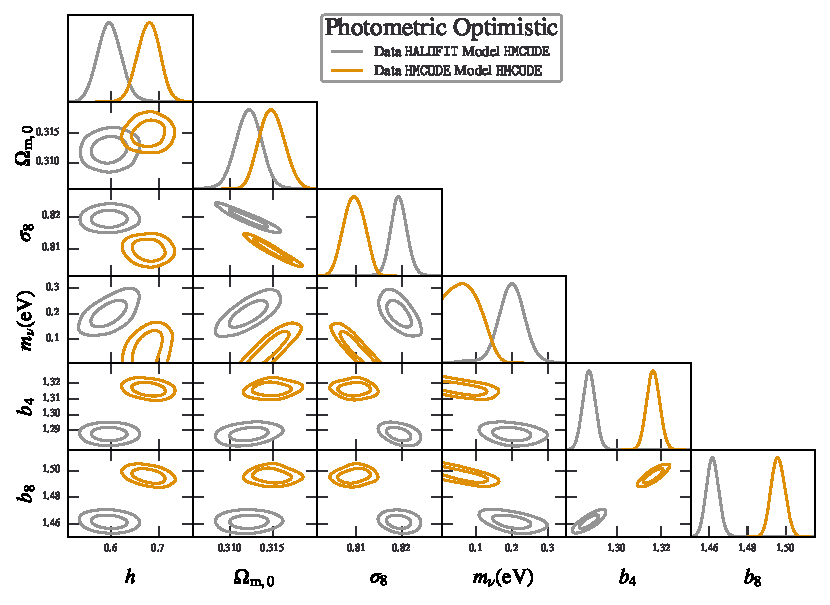
\includegraphics[width=0.9\textwidth]{../plots/P_Halofit_v_P_Hmcode_bias.pdf}
    \label{fig:triangle_HCvHM_biased}
\end{figure}
\begin{figure}
    \centering
    \caption{Same as figure \ref{fig:PcbVPmm} but switching the nonlinear model from \hmcode to \halofit.}
    \begin{subfigure}[b]{0.70\textwidth}
        \centering
        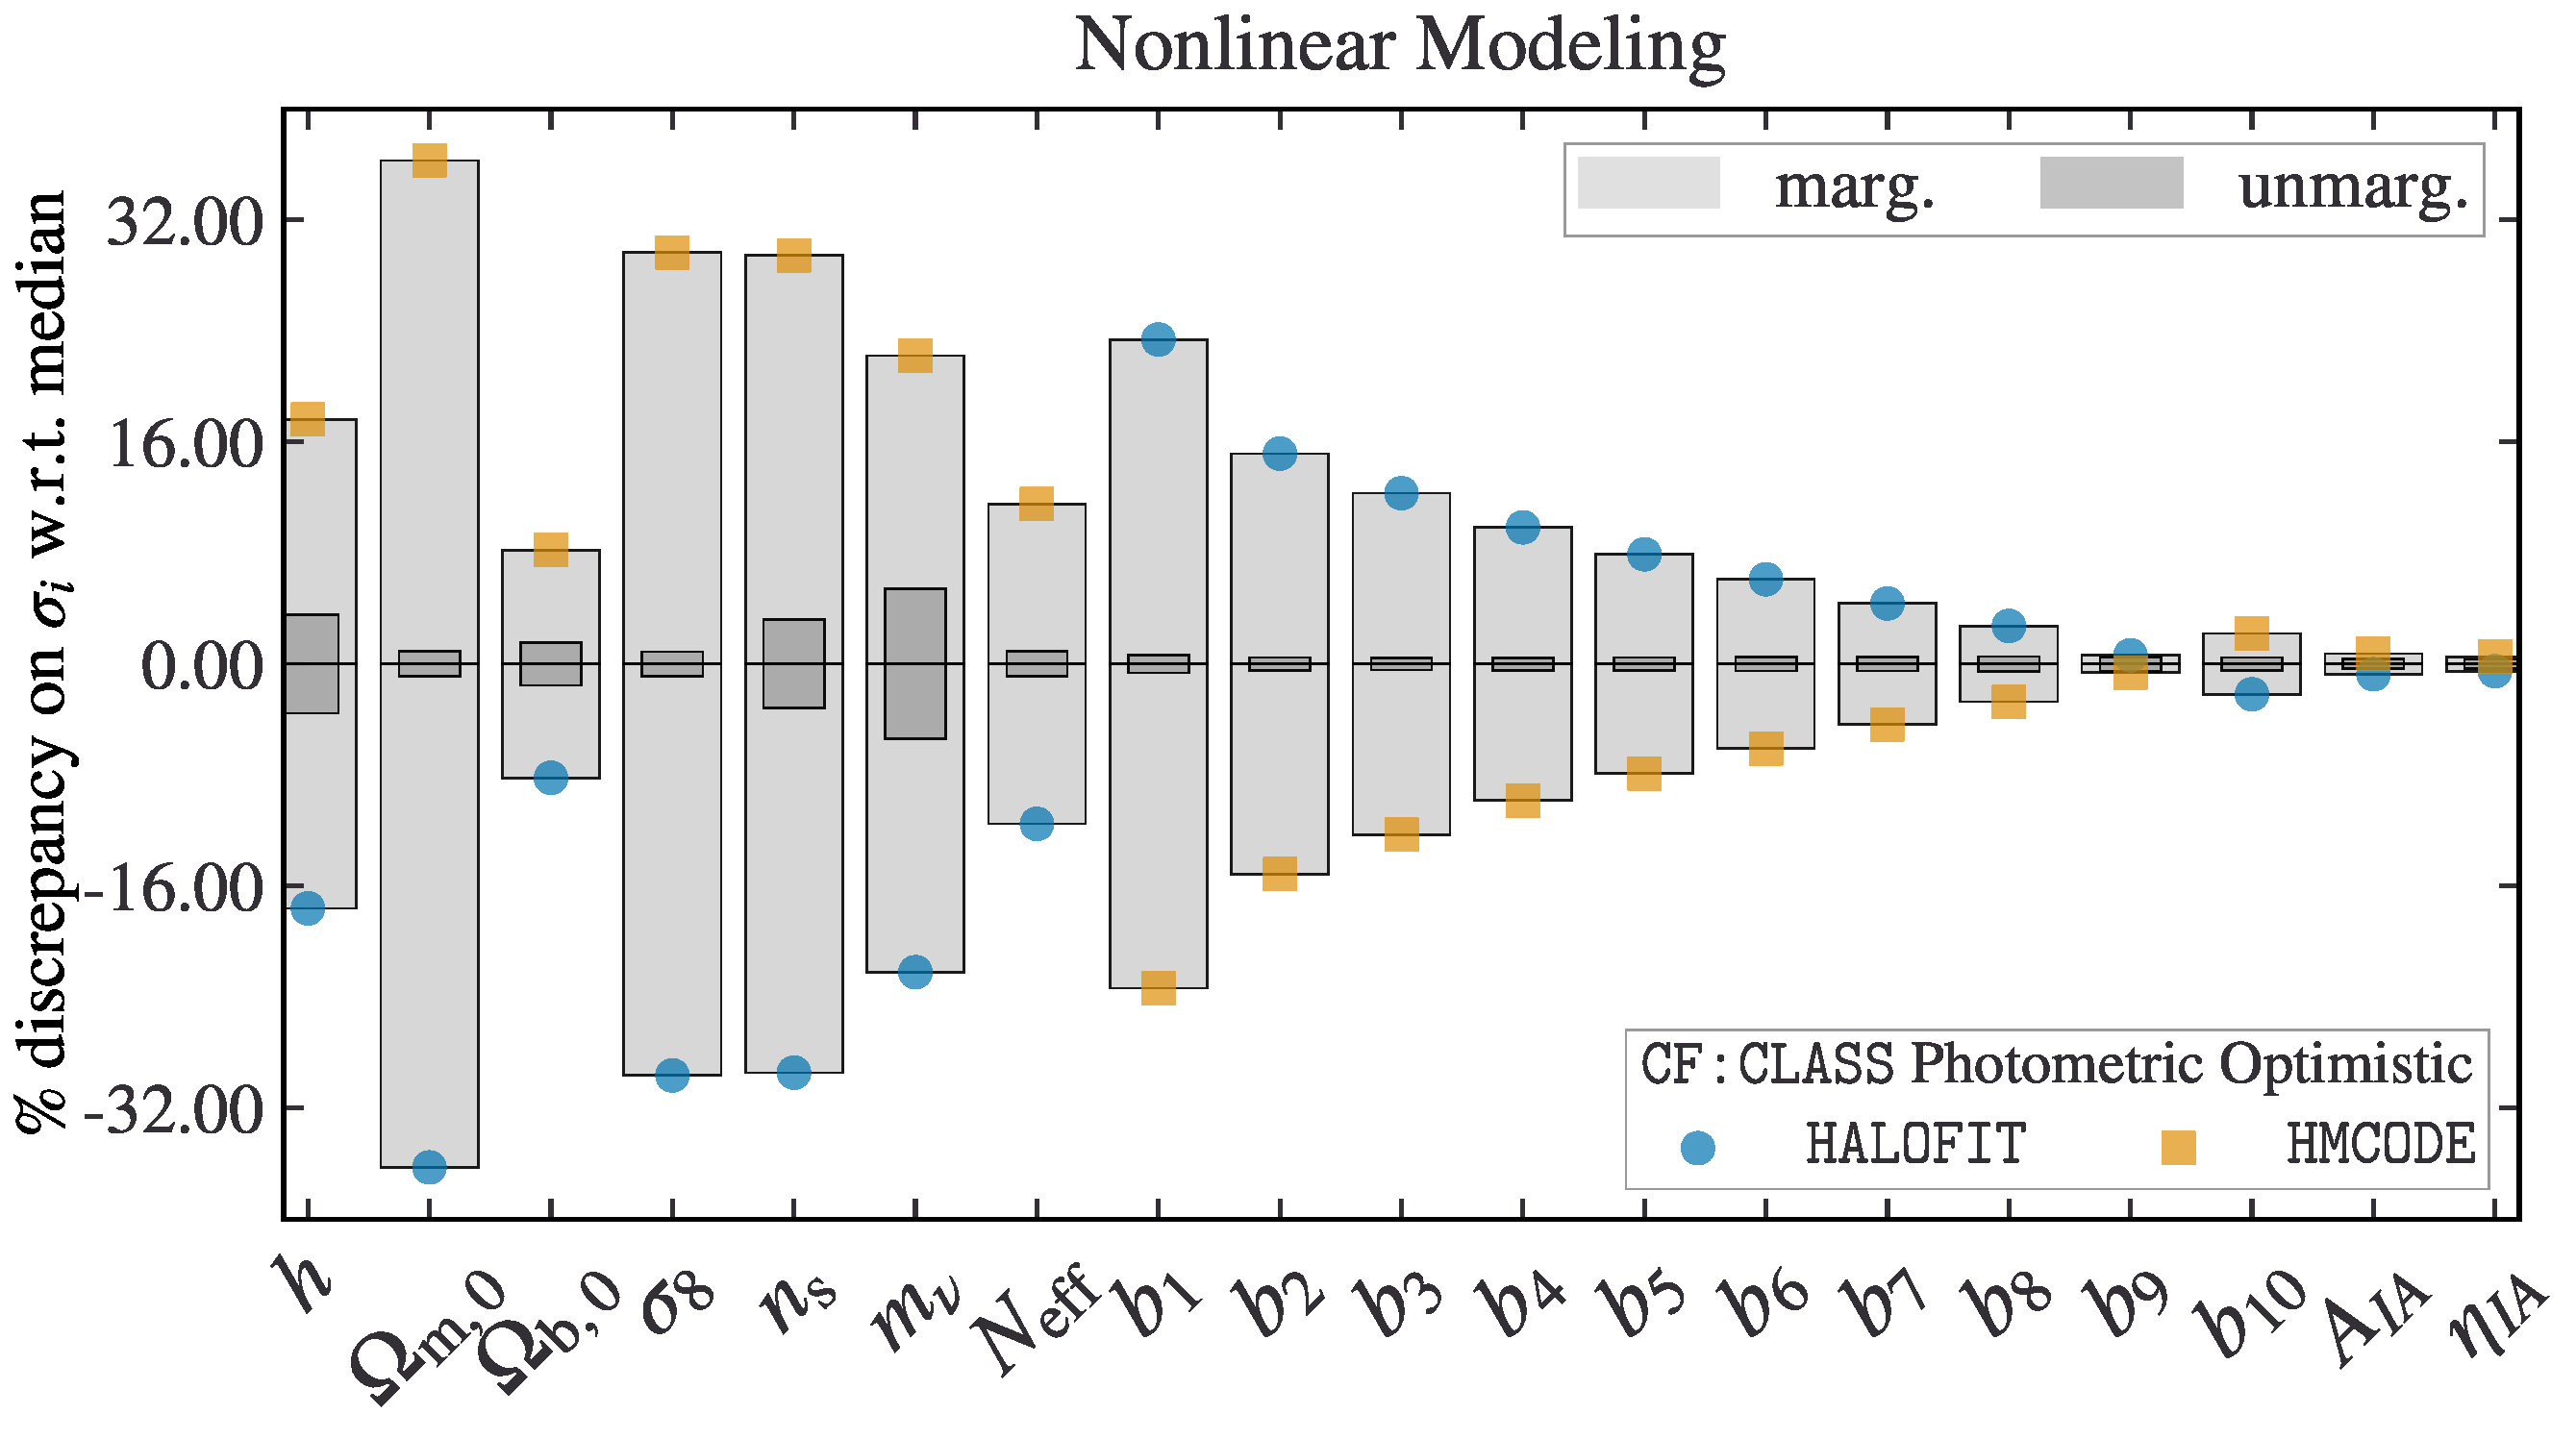
\includegraphics[width=\textwidth]{../plots/cosmopars_HalofitvHMcode_photo_Comparision_error_comparison.pdf}
        \caption{Comparision of the one-dimensional marginalized and unmarginalized errors obtained by using either of the two nonlinear correction codes.}
        \label{fig:dotsHCvHM}
    \end{subfigure}
    \\
    \begin{subfigure}[b]{0.70\textwidth}
        \centering
        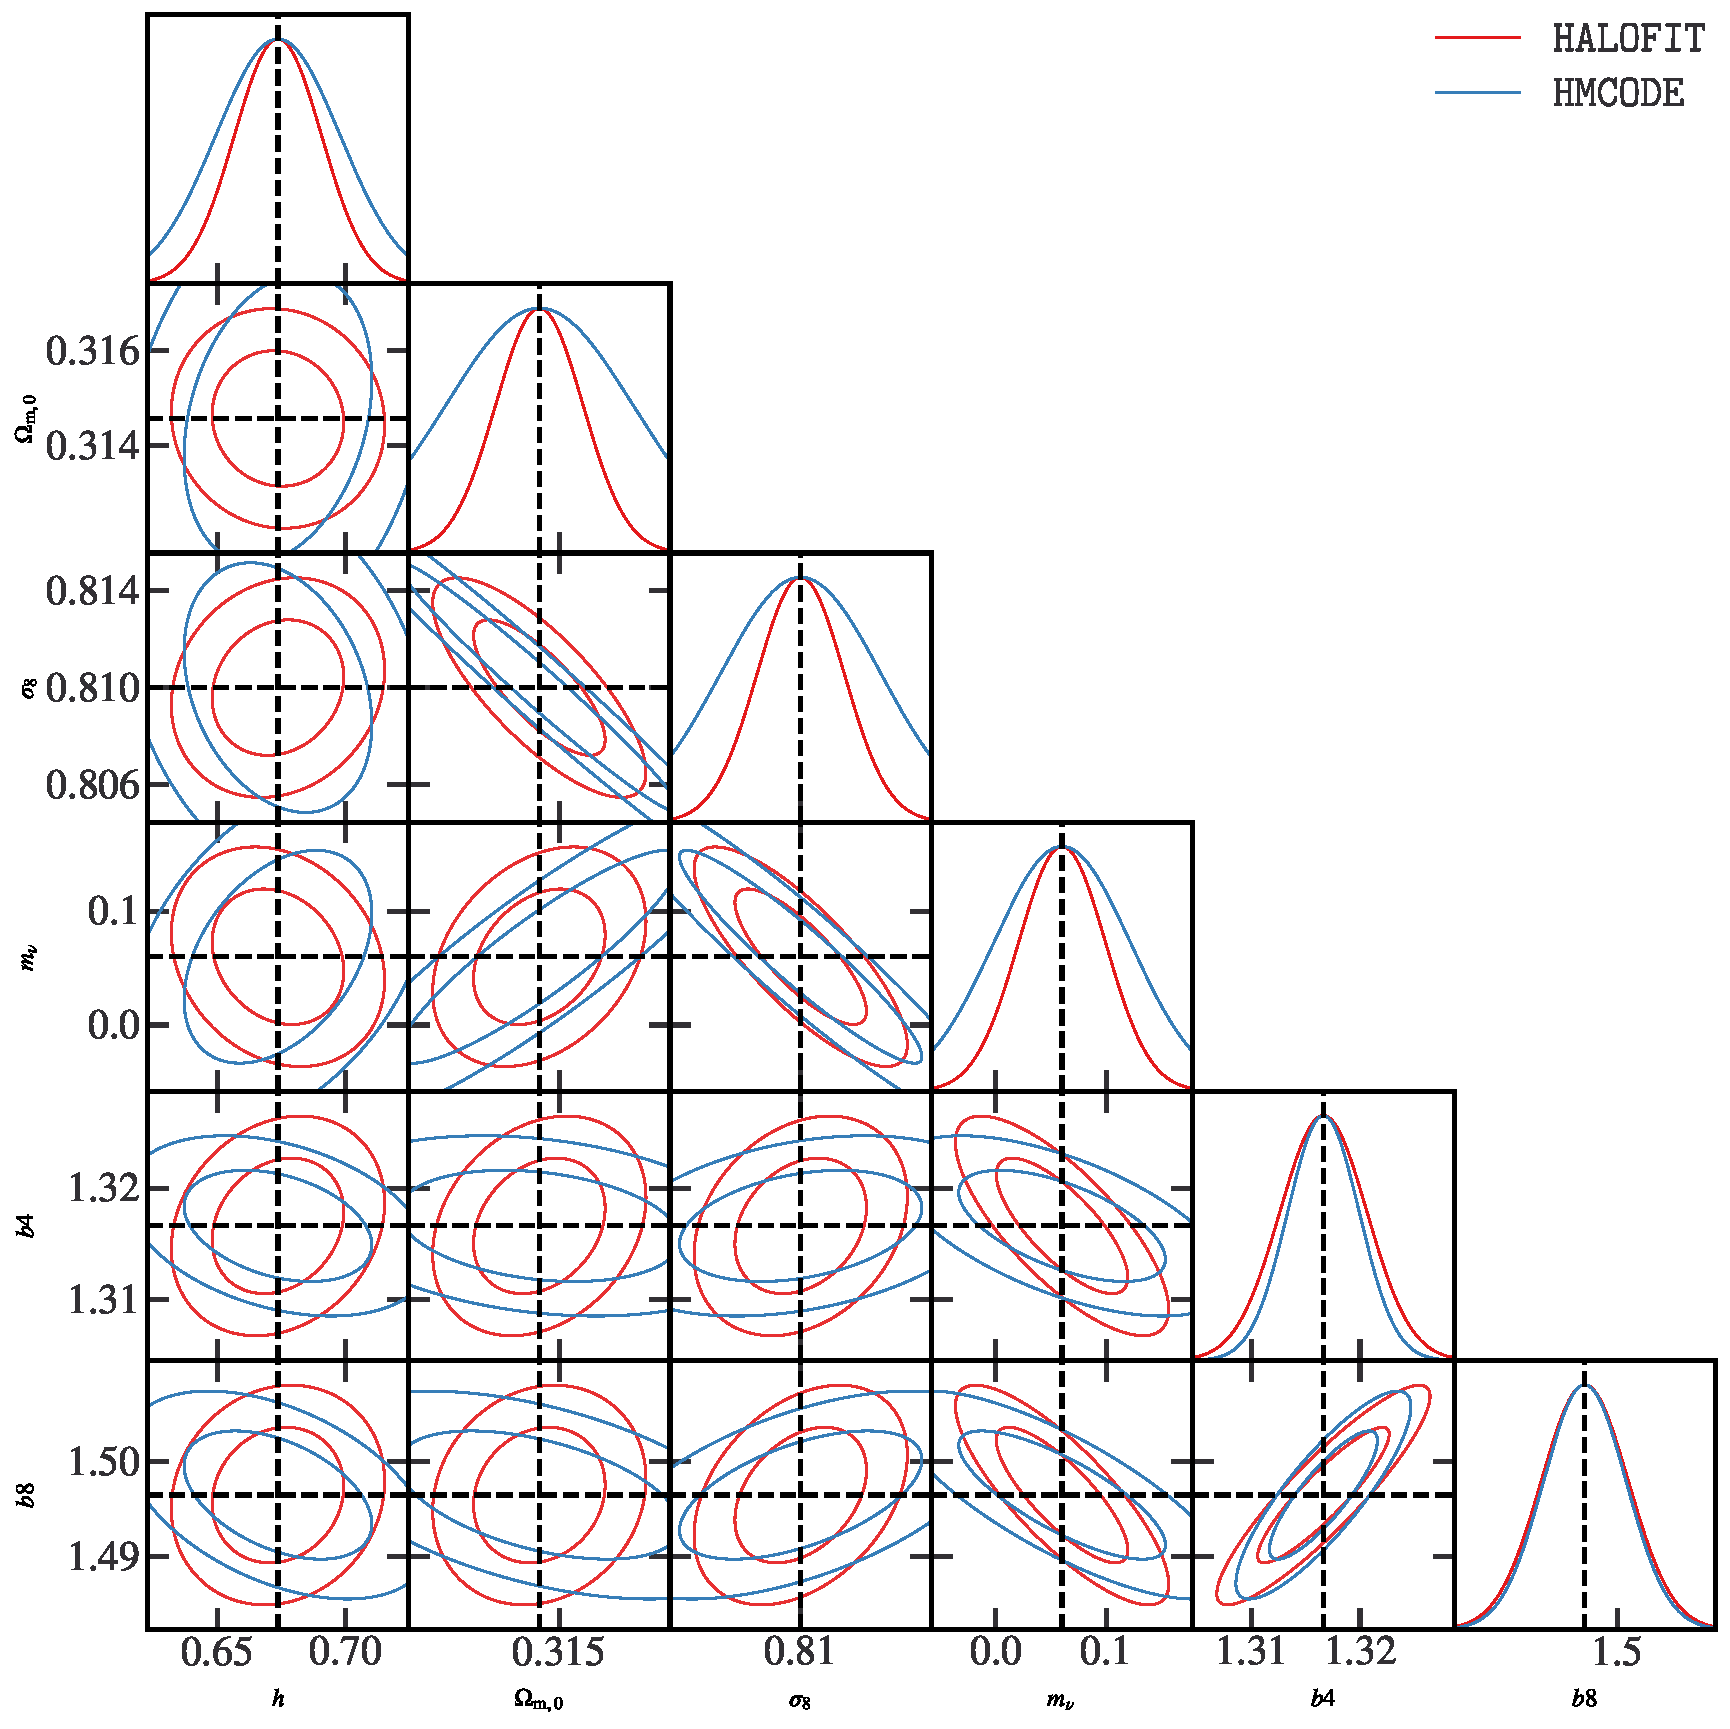
\includegraphics[width=\textwidth]{../plots/less_HalofitvHMcode_photo_Comparision_contours.pdf}
        \caption{Comparision of the one and two-dimensional marginalized contours for the two different nonlinear correction codes. We marginalized other cosmological and nuisance parameters as their trends are the same.}
        \label{fig:triangleHCvHM}
    \end{subfigure}
       \label{fig:HCvHM} 
\end{figure}
\end{document}
